\documentclass[conference]{IEEEtran}

\usepackage[utf8]{inputenc}
\usepackage[T1]{fontenc}
\usepackage[english]{babel}
\usepackage{microtype}
\usepackage{amsmath,amssymb,amsfonts}
\usepackage{siunitx}
\sisetup{
    output-decimal-marker = {.},
    per-mode = symbol,
    range-phrase = { to },
    detect-all
}

\usepackage{graphicx}
\graphicspath{{./}{./figuras/}}
\DeclareGraphicsExtensions{.pdf,.png,.jpg,.jpeg}

\usepackage{tikz}
\usetikzlibrary{arrows.meta, positioning, fit, calc, shapes.geometric, chains, bending, backgrounds}
\pgfdeclarelayer{zonebg}
\pgfdeclarelayer{cardbg}
\pgfdeclarelayer{bg}
\pgfsetlayers{background,zonebg,bg,cardbg,main}

\usepackage{booktabs}
\usepackage{tabularx}
\usepackage{listings}
\usepackage{xcolor}
\usepackage{cite}
\usepackage{xurl}
\usepackage[colorlinks=true, linkcolor=blue!70!black, citecolor=blue!70!black, urlcolor=blue!70!black]{hyperref}

\emergencystretch=3em
\hbadness=10000
\vbadness=10000
\sloppy

\lstdefinelanguage{HTML}{
  morekeywords={html,head,meta,title,style,body,header,div,nav,a,main,section,h1,h2,h3,h4,p,span,img,footer,strong,em},
  sensitive=false,
  morecomment=[s]{<!--}{-->},
  morecomment=[s]{/*}{*/},
  morestring=[b]",
  morestring=[b]'
}

\lstset{
    backgroundcolor=\color{black!3},
    basicstyle=\ttfamily\scriptsize,
    keywordstyle=\color{blue!70!black}\bfseries,
    commentstyle=\color{green!45!black}\itshape,
    stringstyle=\color{orange!65!black},
    frame=single,
    framerule=0.4pt,
    rulecolor=\color{black!35},
    breaklines=true,
    breakatwhitespace=false,
    columns=fullflexible,
    keepspaces=true,
    showstringspaces=false,
    numbers=none,
    xleftmargin=0pt,
    xrightmargin=0pt,
    framexleftmargin=0pt,
    framexrightmargin=0pt,
    captionpos=b,
    abovecaptionskip=6pt,
    belowcaptionskip=8pt,
    literate=
      {á}{{\'a}}1 {é}{{\'e}}1 {í}{{\'i}}1 {ó}{{\'o}}1 {ú}{{\'u}}1
      {Á}{{\'A}}1 {É}{{\'E}}1 {Í}{{\'I}}1 {Ó}{{\'O}}1 {Ú}{{\'U}}1
      {ñ}{{\~n}}1 {Ñ}{{\~N}}1 {ü}{{\"u}}1 {Ü}{{\"U}}1
      {°}{{\textdegree}}1 {–}{{-}}1 {—}{{--}}1 {→}{{->}}1 {←}{{<-}}1
}

\begin{document}

\title{Design, Deployment, and Packet-Level Verification of a ZeroTier SD-WAN and Dual-Intranet HTTPS Infrastructure for International COIL Collaboration}

\author{
    \IEEEauthorblockN{Miguel \'{A}ngel Rodr\'{i}guez Payares and Luis Alejandro Le\'{o}n Vel\'{a}squez}
    \IEEEauthorblockA{
        \textit{Electronic Engineering Program, Faculty of Basic Sciences and Engineering} \\
        \textit{Universidad de los Llanos (UniLlanos), Villavicencio, Meta, Colombia} \\
        \textit{International COIL Module 2 Partner Collaboration with Seneca Polytechnic, Toronto, Canada} \\
        {\small \texttt{marodriguez.payares@unillanos.edu.co} (ID: 161004834) \quad \texttt{laleon.velasquez@unillanos.edu.co}}
    }
}

\maketitle

\begin{abstract}
This engineering report documents the complete design, deployment, live telemetry acquisition, and packet-level verification of a Software-Defined Wide Area Network (SD-WAN) and dual-tenant HTTPS cultural intranet infrastructure developed for Module 2 of the Collaborative Online International Learning (COIL) partnership between Universidad de los Llanos (Villavicencio, Colombia) and Seneca Polytechnic (Toronto, Canada). Five authorized endpoints (desktop hosts and mobile Android devices) were interconnected across a private ZeroTier overlay subnetwork (\texttt{abfd31bd47affa39}, \texttt{172.22.0.0/16}, interface MTU \qty{1300}{\byte}). A custom threaded Python web server (\texttt{COIL-DualIntranet/2.0}) delivers responsive institutional intranets secured with TLS~1.3 (\texttt{TLS\_AES\_256\_GCM\_SHA384}) using a private 2048-bit RSA Root Certificate Authority (\texttt{COIL Group 2 Root CA}) with Subject Alternative Name (SAN) leaf certificates trusted natively by Windows and Android clients for zero-warning browser verification. Domain-based routing (\texttt{www.coil-group2.com}) is served by a \texttt{dnslib}-based authoritative UDP/53 DNS daemon implementing RFC~2308 negative caching (\texttt{NODATA+SOA}). Live Wireshark dissection (\qty{24.81}{\kilo\byte} capture, strictly below the \qty{10}{\mega\byte} limit) validates sub-millisecond (\qty{0.53}{\milli\second}) SD-WAN DNS resolution, MSS~\qty{1260}{\byte} TCP three-way handshakes, 1-RTT TLS~1.3 encrypted delivery of the \qty{15470}{\byte} partner intranet payload, and graceful four-way FIN teardowns with zero resets.
\end{abstract}

\begin{IEEEkeywords}
SD-WAN, ZeroTier, TLS~1.3, Public Key Infrastructure, Authoritative DNS, Wireshark, Deep Packet Inspection, COIL.
\end{IEEEkeywords}

\section{Introduction}
\label{sec:introduction}

Modern academic collaborations increasingly rely on distributed laboratory infrastructures in which students and faculty must securely share private web applications, telemetry, and naming services across institutional boundaries. Within Module~2 of the \textit{Sistemas de Comunicaci\'{o}n~2} course, a Collaborative Online International Learning (COIL) partnership between Universidad de los Llanos (Villavicencio, Meta, Colombia) and Seneca Polytechnic (Toronto, Ontario, Canada) requires interconnecting geographically separated hosts so that participants at each institution can navigate cultural intranet portals deployed by their counterparts.

Directly exposing local development servers across residential and campus networks introduces severe architectural obstacles, including symmetric Network Address Translation (NAT), carrier-grade address sharing, restrictive campus firewalls, and ephemeral public IPv4 leases \cite{tanenbaum2021,kurose2017}. Furthermore, relying on raw IP addresses, unencrypted HTTP transport, or untrusted self-signed certificates degrades usability and fails enterprise security baselines. To overcome these limitations without dedicated site-to-site VPN hardware, COIL Group~2 engineered a unified Software-Defined Wide Area Network (SD-WAN) overlay coupled with a private Public Key Infrastructure (PKI), authoritative DNS resolution, and packet-level forensic validation \cite{zerotier2024}.

The implementation satisfies four measurable engineering objectives:
\begin{enumerate}
    \item \textbf{Private SD-WAN Overlay Interconnection:} Deploy a cryptographically authenticated ZeroTier Layer-2/Layer-3 overlay network over the \texttt{172.22.0.0/16} subnet with an interface Maximum Transmission Unit (MTU) of \qty{1300}{\byte}, strict private admission (\num{5}/\num{10} authorized endpoints, zero unauthorized hosts), explicit student and server labeling, and verified peer-to-peer ICMP reachability \cite{zerotier2024}.
    \item \textbf{Dual Cultural Intranets under HTTPS/TLS~1.3 with Custom Root CA Trust:} Serve responsive institutional cultural intranets for Universidad de los Llanos and Seneca Polytechnic over HTTPS (TLS~1.3) backed by a custom Root Certificate Authority (\texttt{COIL Group 2 Root CA}) installed in client operating system trust stores to eliminate browser security warnings (rubric bonus criterion).
    \item \textbf{Authoritative DNS Domain Resolution:} Operate an authoritative UDP port~53 DNS service resolving institutional project domains (\texttt{www.coil-group2.com} and subdomains) across the SD-WAN mesh while forwarding external queries upstream, eliminating manual IP-based access.
    \item \textbf{Wireshark Packet Forensics ($< \qty{10}{\mega\byte}$):} Capture live HTTPS client-server traffic over the ZeroTier virtual interface into a compact \texttt{.pcapng} trace strictly below \qty{10}{\mega\byte}, verifying TCP three-way handshakes, TLS~1.3 negotiation and encrypted payload delivery, and graceful connection teardowns.
\end{enumerate}

The remainder of this report documents the ZeroTier SD-WAN IP allocation and verification evidence (Rubric Section~I), individual English-narrated demonstration videos (Rubric Section~II), Wireshark packet dissection (Rubric Section~III), step-by-step deployment manuals covering SD-WAN, web hosting, PKI trust, and DNS resolution (Rubric Section~IV), and concluding quantitative findings alongside the complete project source code in the appendices.

\section{ZeroTier SD-WAN IP Assignment and Node Labeling}
\label{sec:zerotier_sdwan}

Addressing Rubric Section~I (\qty{5}{\percent}), this section presents the overlay network architecture, the complete authorized node registry, compliance with student and web-server labeling rules, and empirical reachability measurements across desktop and mobile endpoints. Step-by-step provisioning commands and controller configuration workflows are deferred to Manual~1 in Section~IV to avoid procedural duplication.

\subsection{SD-WAN Overlay Architecture and Addressing Plan}
\label{subsec:sdwan_architecture}

ZeroTier abstracts physical WAN diversity into a flat virtual Ethernet broadcast domain by decoupling the underlay transport (Virtual Layer~1, VL1) from virtualized switching and addressing (Virtual Layer~2, VL2) \cite{zerotier2024}. Each endpoint generates a cryptographic public/private key pair whose hash forms a unique 40-bit (10-hexadecimal-character) Node ID, enabling authenticated UDP encapsulation and NAT hole punching across disparate residential ISPs without central traffic hairpins \cite{zerotier2024,kurose2017}.

For the COIL Group~2 deployment, the private overlay network ``COIL Group 2 SD-WAN - UniLlanos \& Seneca'' was provisioned under Network ID \texttt{abfd31bd47affa39} with \textit{Private} access control enabled, ensuring that packets from unapproved endpoints are dropped at the controller plane. All authorized interfaces operate on the managed IPv4 prefix \texttt{172.22.0.0/16} with a virtual interface MTU of \qty{1300}{\byte}. Selecting a \qty{1300}{\byte} overlay MTU provides sufficient headroom beneath standard \qty{1500}{\byte} physical Ethernet and PPPoE underlay links to accommodate VL1 UDP/cryptographic encapsulation overhead without outer IP fragmentation \cite{tanenbaum2021,zerotier2024}. At the time of verification, the network held \num{5}/\num{10} included device slots, comprising \num{5} authorized nodes and \num{0} unauthorized nodes (\num{3} active desktop hosts and \num{2} inactive mobile devices).

\begin{figure*}[htbp]
\centering
\definecolor{ztInk}{HTML}{0F172A}
\definecolor{ztMuted}{HTML}{475569}
\definecolor{ztCtrlBg}{HTML}{F5F0FF}
\definecolor{ztCtrlLine}{HTML}{6D28D9}
\definecolor{ztCtrlDark}{HTML}{4C1D95}
\definecolor{ztUniBg}{HTML}{EFF6FF}
\definecolor{ztUniLine}{HTML}{1D4ED8}
\definecolor{ztUniDark}{HTML}{1E3A8A}
\definecolor{ztSenBg}{HTML}{ECFDF5}
\definecolor{ztSenLine}{HTML}{047857}
\definecolor{ztSenDark}{HTML}{064E3B}
\definecolor{ztCliBg}{HTML}{FFF7ED}
\definecolor{ztCliLine}{HTML}{C2410C}
\definecolor{ztCliDark}{HTML}{7C2D12}
\definecolor{ztSumBg}{HTML}{F8FAFC}
\definecolor{ztSumLine}{HTML}{64748B}
\definecolor{ztMeshLine}{HTML}{334155}

\resizebox{0.96\textwidth}{!}{%
\begin{tikzpicture}[
    >=Stealth,
    zone box/.style={
        draw=#1, line width=0.85pt, dashed, rounded corners=6pt, inner sep=6pt
    },
    zone hdr/.style={
        font=\scriptsize\bfseries, text=#1, inner xsep=2pt, inner ysep=1.5pt
    },
    card frame/.style={
        draw=#1, line width=0.85pt, rounded corners=4pt, inner sep=4pt, fill=white
    },
    card pill/.style={
        fill=#1, text=white, font=\scriptsize\bfseries,
        rounded corners=2.5pt, inner xsep=5pt, inner ysep=3pt, align=flush left
    },
    card body/.style={
        font=\fontsize{6.8}{9.2}\selectfont, text=ztInk, align=flush left,
        inner xsep=3pt, inner ysep=2.5pt
    },
    p2p link/.style={
        {Stealth[length=5pt,width=4pt]}-{Stealth[length=5pt,width=4pt]},
        line width=1.35pt, shorten >=1.5pt, shorten <=1.5pt
    },
    mesh stub/.style={
        -{Stealth[length=4.5pt,width=3.5pt]},
        line width=1.0pt, color=ztMeshLine, shorten >=1.5pt, shorten <=0pt
    },
    ctrl link/.style={
        -{Stealth[length=4.5pt,width=3.5pt]},
        line width=0.85pt, densely dashed, color=ztCtrlLine,
        rounded corners=4pt, shorten >=1.5pt, shorten <=1pt
    },
    edge badge/.style={
        draw=#1, fill=white, line width=0.65pt, rounded corners=3pt,
        font=\fontsize{6.4}{8.6}\selectfont, text=ztInk, align=center,
        inner xsep=4pt, inner ysep=3pt
    },
    ctrl tag/.style={
        fill=white, text=ztCtrlDark, font=\fontsize{6}{8.0}\selectfont\bfseries,
        inner xsep=3pt, inner ysep=1.5pt, rounded corners=2pt
    }
]

\node[card pill=ztUniDark, text width=4.65cm, anchor=north west] (n1_hdr) at (0,0)
    {Node 1: UniLlanos Primary Host};
\node[card body, text width=4.65cm, below=2pt of n1_hdr.south, anchor=north] (n1_body) {%
    \textbf{Miguel Rodriguez - Unillanos Website Server}\\
    ID: \texttt{AED30A4FDD} (\texttt{aed30a4fdd})\\
    OS: Windows 11 (\texttt{x86\_64})\\
    ZeroTier IP: \texttt{172.22.201.2/16}\\
    Physical IP: \texttt{181.51.34.123}\\
    Services: \texttt{server\_https.py} (TCP \texttt{443} TLS 1.3 \& TCP \texttt{80}),
    \texttt{dns\_server.py} (UDP \texttt{53}), Private Root CA (\texttt{COIL Group 2 Root CA})%
};
\begin{pgfonlayer}{cardbg}
    \node[card frame=ztUniLine, fit=(n1_hdr)(n1_body)] (node1) {};
\end{pgfonlayer}
\node[zone hdr=ztUniDark, anchor=south west] (uni_hdr) at ($(node1.north west) + (0, 3pt)$)
    {UNILLANOS HOST ZONE};
\begin{pgfonlayer}{zonebg}
    \node[zone box=ztUniLine, fill=ztUniBg, fit=(uni_hdr)(node1)] (uni_zone) {};
\end{pgfonlayer}

\node[card pill=ztCliDark, text width=4.15cm, below=2.9cm of node1.south west, anchor=north west] (n3_hdr)
    {Node 3: Partner Student PC};
\node[card body, text width=4.15cm, below=2pt of n3_hdr.south, anchor=north] (n3_body) {%
    \textbf{Luis Alejandro Leon - Student Client}\\
    ID: \texttt{B63D8AEBA8} (\texttt{b63d8aeba8})\\
    OS: Windows (\texttt{x86\_64})\\
    ZeroTier IPs: \texttt{172.22.100.11}, \texttt{172.22.164.74}\\
    Physical IP: \texttt{181.51.34.104}%
};

\node[card pill=ztCliDark, text width=3.8cm, right=0.55cm of n3_hdr.north east, anchor=north west] (n4_hdr)
    {Node 4: Partner Mobile Client};
\node[card body, text width=3.8cm, below=2pt of n4_hdr.south, anchor=north] (n4_body) {%
    \textbf{Luis Alejandro Leon - Student Client}\\
    ID: \texttt{F6FCD4CE4D} (\texttt{f6fcd4ce4d})\\
    OS: Android (\texttt{arm64})\\
    ZeroTier IP: \texttt{172.22.100.10}%
};

\node[card pill=ztCliDark, text width=4.15cm, right=0.55cm of n4_hdr.north east, anchor=north west] (n5_hdr)
    {Node 5: Mobile Verification Client};
\node[card body, text width=4.15cm, below=2pt of n5_hdr.south, anchor=north] (n5_body) {%
    \textbf{Miguel Rodriguez - Student Client}\\
    ID: \texttt{8EB3130D2C} (\texttt{8eb3130d2c})\\
    OS: Android (\texttt{arm64})\\
    ZeroTier IPs: \texttt{172.22.38.108}, \texttt{172.22.201.50}%
};

\path let \p1=(n3_body.south), \p2=(n4_body.south), \p3=(n5_body.south) in
    coordinate (cli_bot) at (0, {min(\y1, min(\y2, \y3))});
\begin{pgfonlayer}{cardbg}
    \node[card frame=ztCliLine, fit=(n3_hdr)(n3_body)(n3_hdr |- cli_bot)] (node3) {};
    \node[card frame=ztCliLine, fit=(n4_hdr)(n4_body)(n4_hdr |- cli_bot)] (node4) {};
    \node[card frame=ztCliLine, fit=(n5_hdr)(n5_body)(n5_hdr |- cli_bot)] (node5) {};
\end{pgfonlayer}
\node[zone hdr=ztCliDark, anchor=south west] (cli_hdr) at ($(node3.north west) + (0, 3pt)$)
    {REMOTE CLIENTS ZONE};
\begin{pgfonlayer}{zonebg}
    \node[zone box=ztCliLine, fill=ztCliBg, fit=(cli_hdr)(node3)(node4)(node5)] (cli_zone) {};
\end{pgfonlayer}

\node[card pill=ztSenDark, text width=4.65cm, anchor=north east] (n2_hdr) at (n1_hdr.north -| n5_hdr.east)
    {Node 2: Seneca Partner Gateway};
\node[card body, text width=4.65cm, below=2pt of n2_hdr.south, anchor=north] (n2_body) {%
    \textbf{Seneca College - Simulated Gateway}\\
    ID: \texttt{1C84E39095} (\texttt{1c84e39095})\\
    OS: Windows 11 (\texttt{x86\_64})\\
    ZeroTier IP: \texttt{172.22.31.69/16}\\
    Physical IP: \texttt{181.51.34.123}\\
    Services: \texttt{server\_https.py} (TCP \texttt{443} TLS 1.3 \& TCP \texttt{80})\\
    Hosts: Seneca Intranet (\texttt{/seneca/})%
};
\path let \p1=(n1_body.south), \p2=(n2_body.south) in
    coordinate (srv_bot) at (0, {min(\y1, \y2)});
\begin{pgfonlayer}{cardbg}
    \node[card frame=ztSenLine, fit=(n2_hdr)(n2_body)(n2_hdr |- srv_bot)] (node2) {};
\end{pgfonlayer}
\node[zone hdr=ztSenDark, anchor=south west] (sen_hdr) at ($(node2.north west) + (0, 3pt)$)
    {SENECA GATEWAY ZONE};
\begin{pgfonlayer}{zonebg}
    \node[zone box=ztSenLine, fill=ztSenBg, fit=(sen_hdr)(node2)] (sen_zone) {};
\end{pgfonlayer}

\node[card body, text width=7.95cm, anchor=south west] (ctrl_c_body) at ($(node1.west |- uni_zone.north) + (0, 1.05cm)$) {%
    \textbf{Network ID:} \texttt{abfd31bd47affa39} \;\textbar\; \textbf{Subnet:} \texttt{172.22.0.0/16} \;\textbar\; \textbf{MTU:} \qty{1300}{\byte}\\
    \textbf{Overlay Transport:} Virtual Ethernet L2/L3 Mesh over UDP port \texttt{9993}%
};
\node[card pill=ztCtrlDark, text width=7.95cm, anchor=south] (ctrl_c_hdr) at ($(ctrl_c_body.north) + (0, 2pt)$)
    {ZeroTier Central Controller (\texttt{my.zerotier.com})};

\node[card pill=ztCtrlDark, text width=4.65cm, anchor=north east] (ctrl_p_hdr) at (ctrl_c_hdr.north -| n2_hdr.east)
    {Planet Root Servers};
\node[card body, text width=4.65cm, below=2pt of ctrl_p_hdr.south, anchor=north] (ctrl_p_body) {%
    \textbf{Root IDs:} \texttt{778cde7190}, \texttt{cafe80ed74}\\
    Peer Discovery, NAT Traversal \& Relay%
};

\path let \p1=(ctrl_c_body.south), \p2=(ctrl_p_body.south) in
    coordinate (ctrl_bot) at (0, {min(\y1, \y2)});
\begin{pgfonlayer}{cardbg}
    \node[card frame=ztCtrlLine, fit=(ctrl_c_hdr)(ctrl_c_body)(ctrl_c_hdr |- ctrl_bot)] (ctrl_central) {};
    \node[card frame=ztCtrlLine, fit=(ctrl_p_hdr)(ctrl_p_body)(ctrl_p_hdr |- ctrl_bot)] (ctrl_planet) {};
\end{pgfonlayer}
\node[zone hdr=ztCtrlDark, anchor=south west] (ctrl_hdr) at ($(ctrl_central.north west) + (0, 3pt)$)
    {CONTROL PLANE \& UNDERLAY DISCOVERY};
\begin{pgfonlayer}{zonebg}
    \node[zone box=ztCtrlLine, fill=ztCtrlBg, fit=(ctrl_hdr)(ctrl_central)(ctrl_planet)] (ctrl_zone) {};
\end{pgfonlayer}

\coordinate (top_mid) at ($(ctrl_zone.north west)!0.5!(ctrl_zone.north east)$);
\node[font=\normalsize\bfseries, text=ztInk, anchor=south] (figtitle) at ($(top_mid) + (0, 0.38cm)$)
    {COIL Group 2 ZeroTier SD-WAN Overlay Topology};

\coordinate (c_n1_x) at ($(n1_hdr.north east) - (0.65cm, 0)$);
\draw[ctrl link] (ctrl_zone.south -| c_n1_x) -- (node1.north -| c_n1_x);
\node[ctrl tag] at ($(ctrl_zone.south -| c_n1_x)!0.5!(uni_zone.north -| c_n1_x)$) {Auth \& Config};

\coordinate (c_n2_x) at ($(n2_hdr.north east) - (0.65cm, 0)$);
\draw[ctrl link] (ctrl_zone.south -| c_n2_x) -- (node2.north -| c_n2_x);
\node[ctrl tag] at ($(ctrl_zone.south -| c_n2_x)!0.5!(sen_zone.north -| c_n2_x)$) {Auth \& Key Dist.};

\coordinate (ctrl_rail_x) at ($(sen_zone.east) + (0.45cm, 0)$);
\draw[ctrl link] (ctrl_zone.east) -- (ctrl_zone.east -| ctrl_rail_x) |- (cli_zone.east);
\node[ctrl tag, align=center] at ($(ctrl_rail_x |- sen_zone.south)!0.5!(ctrl_rail_x |- cli_zone.north)$)
    {Control /\\[1pt]STUN};

\coordinate (lan_mid) at ($(node1.east)!0.5!(node2.west)$);
\draw[p2p link, color=ztSenLine] (node1.east) -- (node2.west);
\node[edge badge=ztSenLine, above=5pt of lan_mid, anchor=south, text width=3.15cm] (lan_top) {%
    \textbf{LAN ZeroTier P2P}\\
    \texttt{192.168.10.x:9993}%
};
\node[edge badge=ztSenLine, below=5pt of lan_mid, anchor=north, text width=3.15cm] (lan_bot) {%
    ICMP avg: \qty{10}{\milli\second} (rev. \qty{6}{\milli\second})\\
    DNS latency: \qty{0.53}{\milli\second}%
};

\coordinate (wan_x) at ($(node3.north east) - (0.35cm, 0)$);
\draw[p2p link, color=ztUniLine] (node1.south -| wan_x) -- (node3.north -| wan_x);
\coordinate (wan_mid) at ($(uni_zone.south -| wan_x)!0.5!(cli_zone.north -| wan_x)$);
\node[edge badge=ztUniLine, left=5pt of wan_mid, anchor=east, text width=3.65cm] (wan_lbl) {%
    \textbf{WAN ZeroTier P2P} (\texttt{181.51.34.104:20594})\\
    ICMP avg: \qty{31}{\milli\second} / \qty{23}{\milli\second} (\qty{0}{\percent} loss)%
};

\coordinate (mesh_y) at ($(uni_zone.south)!0.50!(cli_zone.north)$);
\coordinate (mesh_x1) at ($(node1.south east) - (0.30cm, 0)$);
\coordinate (mesh_x4) at (node4.north);
\coordinate (mesh_x5) at (node5.north);

\draw[line width=1.1pt, color=ztMeshLine] (mesh_x1 |- mesh_y) -- (mesh_x5 |- mesh_y);
\foreach \mx in {mesh_x1, mesh_x4, mesh_x5} {
    \fill[ztMeshLine] (\mx |- mesh_y) circle (1.7pt);
}
\draw[mesh stub] (mesh_x1 |- mesh_y) -- (node1.south -| mesh_x1);
\draw[mesh stub] (mesh_x5 |- mesh_y) -- (node2.south -| mesh_x5);
\draw[mesh stub] (mesh_x4 |- mesh_y) -- (node4.north);
\draw[mesh stub] (mesh_x5 |- mesh_y) -- (node5.north);

\node[edge badge=ztMeshLine, text width=4.3cm] at ($(mesh_x4 |- mesh_y)!0.5!(mesh_x5 |- mesh_y)$) {%
    \textbf{Virtual Ethernet L2/L3 Mesh}\\
    \texttt{172.22.0.0/16} \textbar\ UDP \texttt{9993} \textbar\ MTU \qty{1300}{\byte}%
};

\path let \p1=(cli_zone.west), \p2=(cli_zone.east) in
    node[draw=ztSumLine, fill=ztSumBg, rounded corners=4pt, inner xsep=6pt, inner ysep=5pt,
         text width={(\x2-\x1)-12.85pt}, align=center,
         font=\fontsize{6.6}{9.5}\selectfont, text=ztInk, anchor=north west]
    (sum_bar) at ($(cli_zone.south west) + (0, -0.32cm)$) {%
        {\fontsize{6.6}{9.6}\selectfont
        \textbf{Verified Overlay Summary:}~
        Network \texttt{abfd31bd47affa39} (\texttt{172.22.0.0/16}, MTU \qty{1300}{\byte})
        \;\textbar\;
        \textbf{LAN P2P:} \qty{10}{\milli\second} / rev. \qty{6}{\milli\second}, DNS \qty{0.53}{\milli\second}\\[2pt]
        \textbf{WAN P2P:} \qty{31}{\milli\second} / \qty{23}{\milli\second} (\qty{0}{\percent} loss)
        \;\textbar\;
        \textbf{Security Stack:} TLS 1.3 (TCP \texttt{443}) + \texttt{COIL Group 2 Root CA}\par}%
    };

\matrix[ampersand replacement=\&, below=0.22cm of sum_bar.south, anchor=north, column sep=7pt, inner sep=0pt,
        nodes={font=\fontsize{6.5}{8.6}\selectfont, text=ztMuted, inner sep=1pt, anchor=west}] (legend_mat) {
    \node[font=\fontsize{6.5}{8.6}\selectfont\bfseries, text=ztInk] {Legend:}; \&
    \node[draw=ztCtrlLine, fill=ztCtrlBg, minimum width=0.28cm, minimum height=0.22cm, rounded corners=1pt] {}; \&
    \node {Control Plane}; \&
    \node[draw=ztUniLine, fill=ztUniBg, minimum width=0.28cm, minimum height=0.22cm, rounded corners=1pt] {}; \&
    \node {UniLlanos Host}; \&
    \node[draw=ztSenLine, fill=ztSenBg, minimum width=0.28cm, minimum height=0.22cm, rounded corners=1pt] {}; \&
    \node {Seneca Gateway}; \&
    \node[draw=ztCliLine, fill=ztCliBg, minimum width=0.28cm, minimum height=0.22cm, rounded corners=1pt] {}; \&
    \node {Remote Clients}; \&
    \node[minimum width=0.45cm, minimum height=0.2cm] (leg_c) {}; \&
    \node {Control Signaling}; \&
    \node[minimum width=0.45cm, minimum height=0.2cm] (leg_p) {}; \&
    \node {P2P / Mesh Link}; \\
};
\draw[ctrl link, shorten >=0pt, shorten <=0pt] (leg_c.west) -- (leg_c.east);
\draw[p2p link, color=ztSenLine, shorten >=0pt, shorten <=0pt] (leg_p.west) -- (leg_p.east);

\end{tikzpicture}%
}
\caption{COIL Group 2 ZeroTier SD-WAN overlay network architecture (\texttt{abfd31bd47affa39}, \texttt{172.22.0.0/16}, MTU \qty{1300}{\byte}). The control plane (\texttt{my.zerotier.com} and Planet root servers) coordinates cryptographic authorization and NAT traversal over UDP/9993, interconnecting the UniLlanos primary server (\texttt{172.22.201.2}), the Seneca Polytechnic gateway (\texttt{172.22.31.69}), and partner desktop/mobile clients.}
\label{fig:sdwan_topology}
\end{figure*}


As illustrated in Fig.~\ref{fig:sdwan_topology}, the virtual \texttt{172.22.0.0/16} switching fabric logically unifies the UniLlanos multi-tenant HTTPS and authoritative DNS host (\texttt{172.22.201.2/16}), the simulated Seneca Polytechnic gateway (\texttt{172.22.31.69/16}), and the remote student desktop and Android clients across physical WAN boundaries.

\subsection{Authorized Member Registry and Node Labeling Compliance}
\label{subsec:member_registry}

Rubric Section~I mandates that every group member connect a host to the SD-WAN, that each node carry an explicit label bearing the corresponding student's name, and that the web server host explicitly declare its hosting role. Table~\ref{tab:zerotier_members} compiles the authoritative registry of all five enrolled endpoints observed in ZeroTier Central.

\begin{table*}[t]
\centering
\caption{ZeroTier Central Authorized Member Registry for Network \texttt{abfd31bd47affa39} (\texttt{COIL Group 2 SD-WAN - UniLlanos \& Seneca}).}
\label{tab:zerotier_members}
\resizebox{\textwidth}{!}{%
\begin{tabular}{@{}lllllll@{}}
\toprule
\textbf{Node ID / Virtual MAC} & \textbf{Assigned Label / Role} & \textbf{OS / Arch (Client)} & \textbf{Managed Overlay IP(s)} & \textbf{Physical Endpoint} & \textbf{Auth} & \textbf{Activity (Last Seen)} \\
\midrule
\begin{tabular}[c]{@{}l@{}}\texttt{1c84e39095}\\{\scriptsize\texttt{3a:e6:2b:a4:2d:a4}}\end{tabular} &
\texttt{Seneca College - Simulated Gateway} &
Windows \texttt{x86\_64} (\texttt{v1.16.2}) &
\texttt{172.22.31.69/16} &
\texttt{181.51.34.123} &
Yes &
Active (\qty{1}{\minute}) \\
\addlinespace[3pt]
\begin{tabular}[c]{@{}l@{}}\texttt{aed30a4fdd}\\{\scriptsize\texttt{3a:54:7c:4d:f2:ec}}\end{tabular} &
\texttt{Miguel Rodriguez - Unillanos Website Server} &
Windows \texttt{x86\_64} (\texttt{v1.16.2}) &
\texttt{172.22.201.2/16} &
\texttt{181.51.34.123} &
Yes &
Active (\qty{1}{\minute}) \\
\addlinespace[3pt]
\begin{tabular}[c]{@{}l@{}}\texttt{b63d8aeba8}\\{\scriptsize\texttt{3a:4c:92:cd:56:99}}\end{tabular} &
\texttt{Luis Alejandro Leon - Student Client} &
Windows \texttt{x86\_64} (\texttt{v1.16.2}) &
\begin{tabular}[c]{@{}l@{}}\texttt{172.22.100.11}\\\texttt{172.22.164.74}\end{tabular} &
\texttt{181.51.34.104} &
Yes &
Active (\qty{1}{\minute}) \\
\addlinespace[3pt]
\begin{tabular}[c]{@{}l@{}}\texttt{8eb3130d2c}\\{\scriptsize\texttt{3a:74:1c:54:b0:1d}}\end{tabular} &
\texttt{Miguel Rodriguez - Student Client} &
Android \texttt{arm64} (\texttt{v1.16.0}) &
\begin{tabular}[c]{@{}l@{}}\texttt{172.22.38.108}\\\texttt{172.22.201.50}\end{tabular} &
\texttt{181.51.34.123} &
Yes &
Inactive (\qty{2}{\hour}) \\
\addlinespace[3pt]
\begin{tabular}[c]{@{}l@{}}\texttt{f6fcd4ce4d}\\{\scriptsize\texttt{3a:0c:53:93:73:7c}}\end{tabular} &
\texttt{Luis Alejandro Leon - Student Client} &
Android \texttt{arm64} (\texttt{v1.16.0}) &
\texttt{172.22.100.10} &
\texttt{181.51.34.104} &
Yes &
Inactive (\qty{37}{\minute}) \\
\bottomrule
\end{tabular}%
}
\end{table*}

\begin{figure*}[t]
\centering
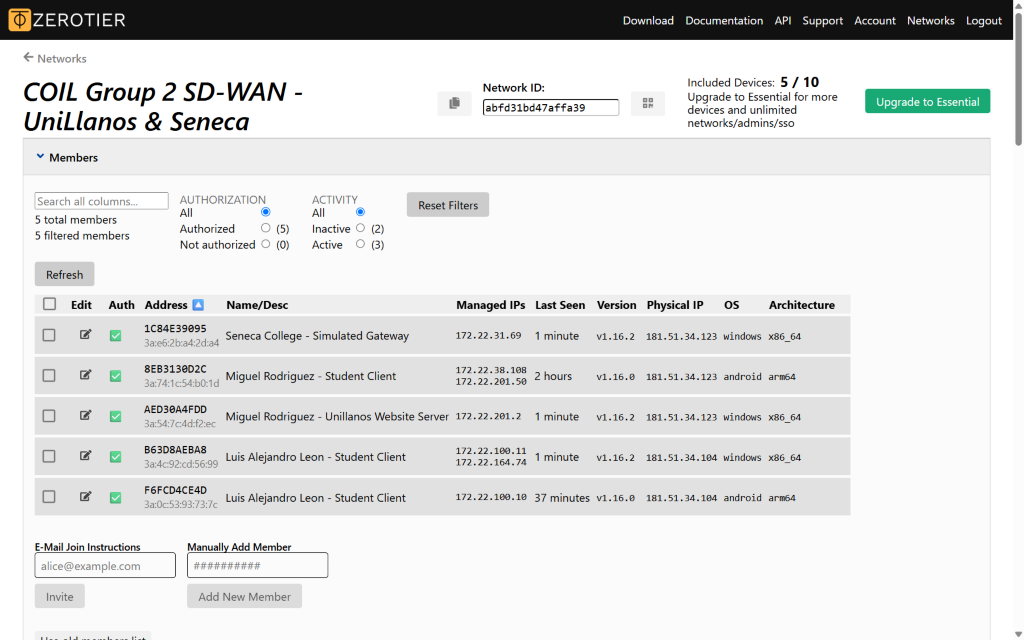
\includegraphics[width=0.92\textwidth]{figuras/zerotier_members_fresh.png}
\caption{ZeroTier Central member management console for Network ID \texttt{abfd31bd47affa39}, confirming \num{5}/\num{10} included devices, \num{5} authorized nodes (\num{0} unauthorized), institutional node labeling, managed \texttt{172.22.x.x} IP assignments, and underlay public endpoints.}
\label{fig:zerotier_members}
\end{figure*}

Fig.~\ref{fig:zerotier_members} corroborates every entry in Table~\ref{tab:zerotier_members} directly from the ZeroTier Central web console. Notice that all five green authorization checkboxes are active (\textit{Authorized (5)}, \textit{Not authorized (0)}), while the activity filter reflects three active Windows~\texttt{x86\_64} nodes running ZeroTier~\texttt{v1.16.2} (seen \qty{1}{\minute} prior) and two Android~\texttt{arm64} handsets running \texttt{v1.16.0} (last seen \qty{37}{\minute} and \qty{2}{\hour} prior). Node \texttt{aed30a4fdd} explicitly identifies its hosting role (``Miguel Rodriguez - Unillanos Website Server'') at \texttt{172.22.201.2/16}, whereas \texttt{1c84e39095} fulfills the simulated partner endpoint role (``Seneca College - Simulated Gateway'') at \texttt{172.22.31.69/16}. Both students also maintain dedicated client workstations and Android test devices under their full names (``Luis Alejandro Leon - Student Client'' and ``Miguel Rodriguez - Student Client''). Examining the underlay column confirms two distinct public ISP ingress addresses (\texttt{181.51.34.123} and \texttt{181.51.34.104}), verifying real cross-ISP WAN operation between the server host and Luis Alejandro Le\'{o}n's client nodes. Two multi-leased nodes (\texttt{b63d8aeba8} and \texttt{8eb3130d2c}) retain secondary \texttt{172.22.x.x} leases in the controller database from prior interface re-bindings, whereas the server and gateway maintain deterministic single-address leases.

\subsection{Host Interface Verification and ICMP Reachability}
\label{subsec:icmp_reachability}

Controller-side IP allocation must match the virtual network interface state bound inside each host operating system. Fig.~\ref{fig:host_ip_verification} documents the local host interface verification confirming that the virtual ZeroTier adapter binds the assigned \texttt{172.22.0.0/16} address and prefix mask locally without conflicting with physical Ethernet or Wi-Fi adapters.

\begin{figure*}[t]
\centering
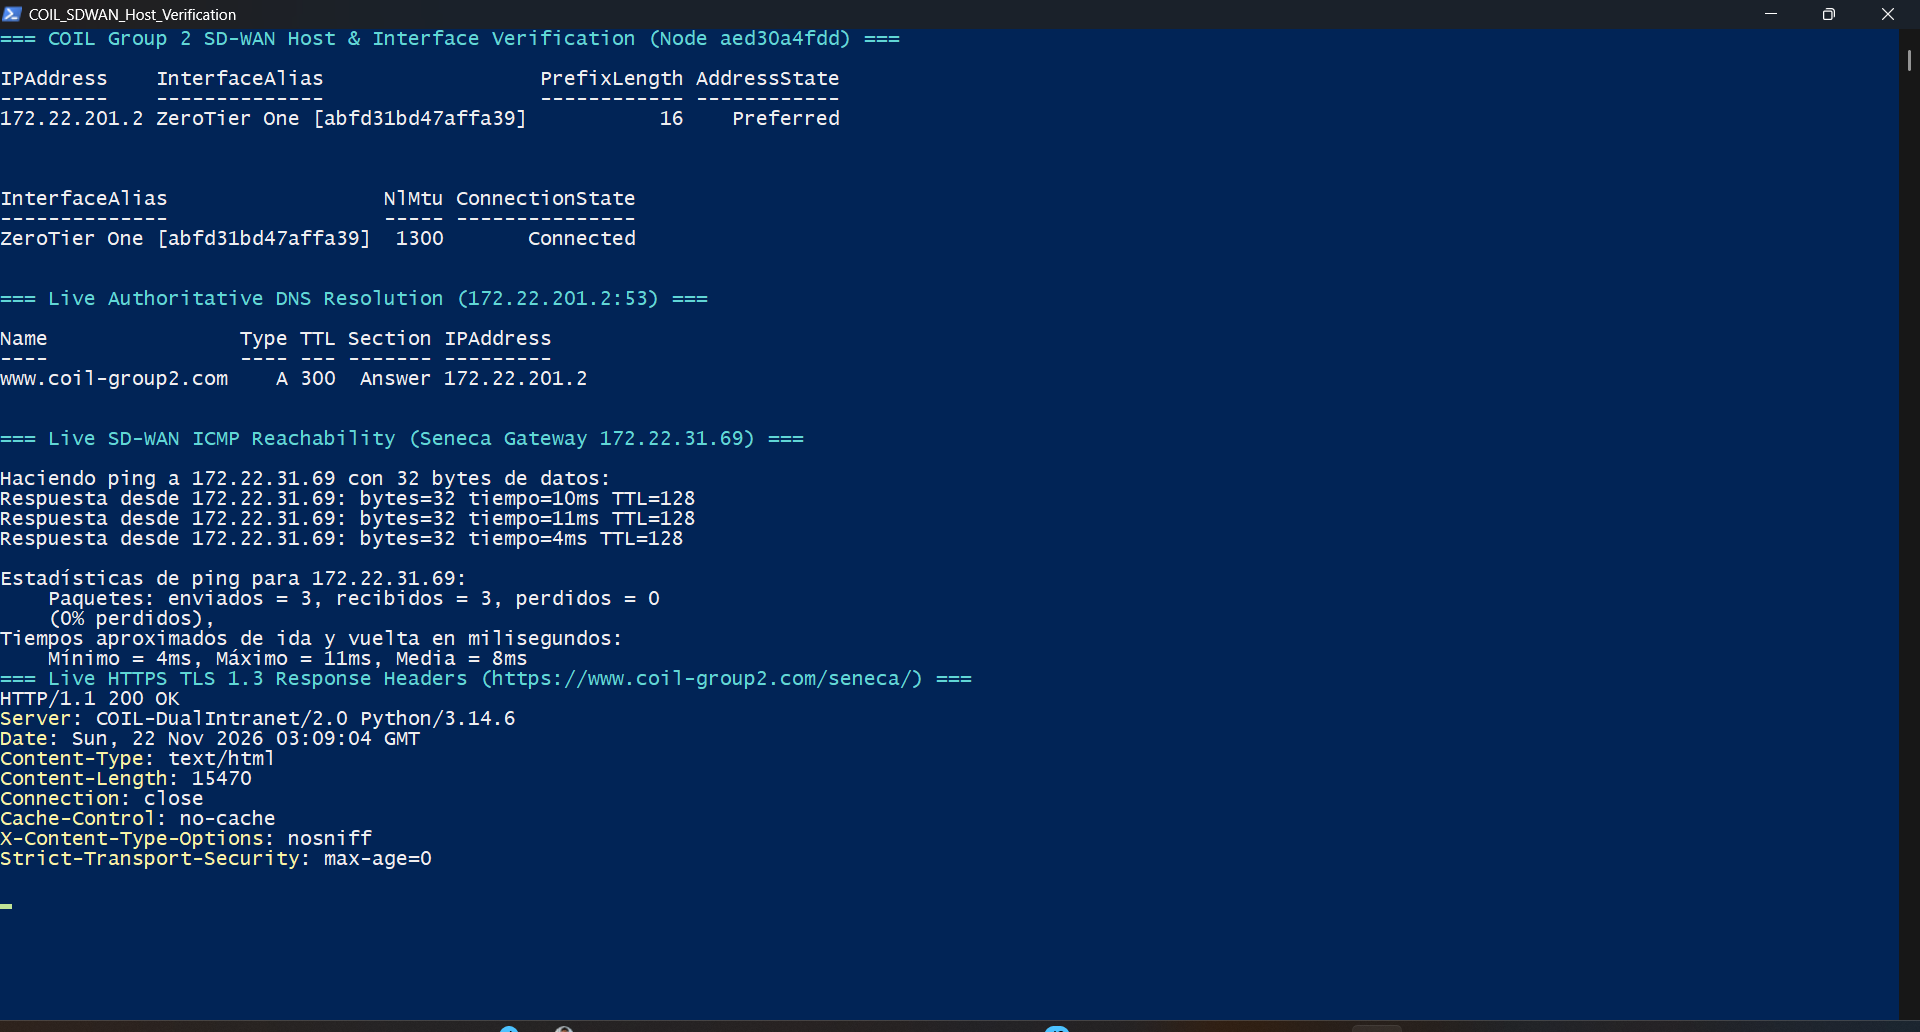
\includegraphics[width=0.92\textwidth]{figuras/host_ip_verification_fresh.png}
\caption{Local host network interface verification confirming active ZeroTier One virtual adapter binding within the \texttt{172.22.0.0/16} SD-WAN overlay subnet.}
\label{fig:host_ip_verification}
\end{figure*}

To verify bidirectional Layer-3 forwarding across the encrypted SD-WAN mesh, live ICMP echo probes were executed from the UniLlanos web server (\texttt{172.22.201.2}) and the simulated Seneca gateway (\texttt{172.22.31.69}) toward both local and remote participant IP addresses. Table~\ref{tab:icmp_rtt} summarizes the measured round-trip time (RTT) distributions and packet-loss ratios.

\begin{table}[t]
\centering
\caption{Live ICMP Round-Trip Time (RTT) and Packet Loss Verification Across the ZeroTier SD-WAN.}
\label{tab:icmp_rtt}
\resizebox{\columnwidth}{!}{%
\begin{tabular}{@{}llcccc@{}}
\toprule
\textbf{Probe Path (Src $\rightarrow$ Dst)} & \textbf{Link Type} & \textbf{Min} & \textbf{Max} & \textbf{Avg} & \textbf{Loss} \\
\midrule
\texttt{172.22.201.2} $\rightarrow$ \texttt{172.22.31.69} & LAN P2P & \qty{3}{\milli\second} & \qty{31}{\milli\second} & \qty{10}{\milli\second} & \qty{0}{\percent} \\
\texttt{172.22.31.69} $\rightarrow$ \texttt{172.22.201.2} & LAN P2P (rev.) & \qty{3}{\milli\second} & \qty{10}{\milli\second} & \qty{6}{\milli\second} & \qty{0}{\percent} \\
\texttt{172.22.201.2} $\rightarrow$ \texttt{172.22.100.11} & WAN P2P & \qty{16}{\milli\second} & \qty{70}{\milli\second} & \qty{31}{\milli\second} & \qty{0}{\percent} \\
\texttt{172.22.201.2} $\rightarrow$ \texttt{172.22.164.74} & WAN P2P & \qty{19}{\milli\second} & \qty{28}{\milli\second} & \qty{23}{\milli\second} & \qty{0}{\percent} \\
\texttt{172.22.201.2} $\rightarrow$ \texttt{172.22.100.10} & Android idle\textsuperscript{*} & -- & -- & -- & \qty{75}{\percent} \\
\bottomrule
\end{tabular}%
}
\vspace{3pt}
\par\noindent\parbox{\columnwidth}{\footnotesize\textsuperscript{*}1/4 packets received; \textit{Destination Host Unreachable} observed while the mobile screen remained locked.}
\end{table}

The telemetry in Table~\ref{tab:icmp_rtt} reveals three distinct operational regimes across the overlay topology:
\begin{enumerate}
    \item \textbf{Local Peer-to-Peer (LAN P2P) Forwarding:} Forward and reverse probes between \texttt{172.22.201.2} and \texttt{172.22.31.69} achieve \qty{0}{\percent} packet loss with a minimum RTT of \qty{3}{\milli\second} and average RTTs of \qty{10}{\milli\second} (forward) and \qty{6}{\milli\second} (reverse). Because both Windows nodes sit behind the same physical endpoint (\texttt{181.51.34.123}), ZeroTier VL1 resolves a direct local UDP path without traversing external root relays \cite{zerotier2024}.
    \item \textbf{Cross-ISP Peer-to-Peer (WAN P2P) Tunneling:} Probes from \texttt{172.22.201.2} (\texttt{181.51.34.123}) to both managed addresses of Luis Alejandro Le\'{o}n's Windows client (\texttt{172.22.100.11} and \texttt{172.22.164.74} behind \texttt{181.51.34.104}) record \qty{0}{\percent} loss with average RTTs of \qty{31}{\milli\second} (range \qtyrange{16}{70}{\milli\second}) and \qty{23}{\milli\second} (range \qtyrange{19}{28}{\milli\second}), respectively. These sub-\qty{35}{\milli\second} averages confirm direct encrypted UDP traversal across distinct ISP networks.
    \item \textbf{Mobile Power-Management Behavior:} Probing the Android handset at \texttt{172.22.100.10} (node \texttt{f6fcd4ce4d}, marked inactive \qty{37}{\minute} prior in Fig.~\ref{fig:zerotier_members}) produced \qty{75}{\percent} packet loss (\num{1}/\num{4} echo replies received, with \textit{Destination Host Unreachable} reported while the screen was locked). This behavior reflects Android background VPN sleep throttling rather than an SD-WAN addressing fault, as active screen interaction restores immediate Layer-3 reachability for mobile HTTPS and root CA verification.
\end{enumerate}

\section{Individual Demonstration Videos}
\label{sec:demo_videos}

Rubric Section~II allocates \qty{10}{\percent} of the Module~2 evaluation weight to individual English-language demonstration videos recorded independently by each group member. Rather than permitting shared group screencasts or numeric IP navigation, the activity specification mandates that each student establish an authenticated Software-Defined Wide Area Network (SD-WAN) session from their personal endpoint, access the partner institution's intranet strictly via its Fully Qualified Domain Name (FQDN) URL (\texttt{https://\allowbreak www.coil-group2.com/\allowbreak seneca/}), verify transport security, and narrate the partner cultural modules in English (spoken narration or synchronized English Text-to-Speech synthesis).

For Universidad de los Llanos participants, the target demonstration portal is the Seneca Polytechnic cultural intranet (\texttt{https://\allowbreak www.coil-group2.com/\allowbreak seneca/}), complementing the reciprocal verification performed by Seneca Polytechnic partners toward the Universidad de los Llanos portal. Requiring domain-based addressing instead of raw IPv4 literals exercises the full application-delivery stack: local DNS resolution over UDP port~53~\cite{rfc1035}, HTTP \texttt{Host} header preservation for multi-tenant path routing under RFC~9110~\cite{rfc9110}, and TLS~1.3 Server Name Indication (SNI) validation against X.509 Subject Alternative Name (SAN) records under RFC~8446 and RFC~5280~\cite{rfc8446,rfc5280}.

\begin{table*}[t]
\centering
\caption{Individual Demonstration Video Deliverables, Target Intranet URLs, Local Archives, and Restricted Hosting Slots}
\label{tab:demo_videos}
\footnotesize
\setlength{\tabcolsep}{4pt}
\renewcommand{\arraystretch}{1.25}
\begin{tabularx}{\textwidth}{
  >{\raggedright\arraybackslash}p{3.45cm}
  >{\raggedright\arraybackslash}p{2.05cm}
  >{\raggedright\arraybackslash}p{3.65cm}
  >{\raggedright\arraybackslash}X
  >{\raggedright\arraybackslash}p{3.15cm}
}
\toprule
\textbf{Student \& Identifier} & \textbf{Institution} & \textbf{Target Intranet \& URL} & \textbf{Local Archive \& Script Reference} & \textbf{Delivery Link (Unlisted / Restricted)} \\
\midrule
\textbf{Miguel \'{A}ngel Rodr\'{i}guez Payares}\newline ID: \texttt{161004834} & Universidad de los Llanos & Seneca Polytechnic Intranet\newline \texttt{https://\allowbreak www.coil-group2.com/\allowbreak seneca/} & Archive: \texttt{modulo2/\allowbreak video/\allowbreak grabaciones/} (\texttt{20261121\_192309.mp4}--\texttt{20261121\_192830.mp4}); compiled demo: \texttt{COIL\_Module2\_\allowbreak Miguel\_Rodriguez\_\allowbreak Demo.mp4}; script: \texttt{modulo2/\allowbreak video/\allowbreak video\_script\_\allowbreak english.md} & \url{https://youtu.be/jrUnb2pqvwg}\newline (YouTube Unlisted) \\
\addlinespace[4pt]
\textbf{Luis Alejandro Le\'{o}n Vel\'{a}squez}\newline \texttt{laleon.velasquez@\allowbreak unillanos.edu.co} & Universidad de los Llanos & Seneca Polytechnic Intranet\newline \texttt{https://\allowbreak www.coil-group2.com/\allowbreak seneca/} & Script Ref.: \texttt{modulo2/\allowbreak video/\allowbreak video\_script\_\allowbreak english.md} (Part~2) & \texttt{[Insert Unlisted YouTube or Google Drive URL]} \\
\bottomrule
\end{tabularx}
\end{table*}

Table~\ref{tab:demo_videos} summarizes the individual video deliverables, institutional affiliations, target partner URLs, local repository archives, and instructor-restricted delivery slots for both Universidad de los Llanos authors.

\subsection{Standardized Four-Scene English Demonstration Protocol}
\label{subsec:video_protocol}

To guarantee technical consistency and complete rubric coverage across both submissions, a unified four-scene demonstration script (\texttt{modulo2/\allowbreak video/\allowbreak video\_script\_\allowbreak english.md}) was authored with a target runtime of \qtyrange{90}{120}{\second} (\mbox{1:30--2:00~min}; paced at \mbox{1:55~min}). Each recording executes the following deterministic verification sequence:

\begin{enumerate}
    \item \textbf{Scene~1 (0:00--0:25) --- Student Introduction and ZeroTier Overlay IP Confirmation:} The student opens the recording in English, stating their full name, Electronic Engineering affiliation at Universidad de los Llanos (Villavicencio, Colombia), and the international COIL Module~2 scope with Seneca Polytechnic. Simultaneously, the screen displays the active ZeroTier One client or terminal interface verifying authorization in private SD-WAN network \texttt{abfd31bd47affa39} (\textit{COIL Group 2 SD-WAN - UniLlanos \& Seneca}) and confirming the host's assigned overlay IPv4 lease inside \texttt{172.22.0.0/16}---\texttt{172.22.201.2} for Miguel \'{A}ngel Rodr\'{i}guez Payares (host node \texttt{AED30A4FDD}) and \texttt{172.22.100.11} for Luis Alejandro Le\'{o}n Vel\'{a}squez (Windows client node \texttt{B63D8AEBA8})~\cite{zerotier2024}.

    \item \textbf{Scene~2 (0:25--0:40) --- Domain-Based Navigation to Seneca Intranet:} Focusing on the browser address bar, the student manually enters \texttt{https://\allowbreak www.coil-group2.com/\allowbreak seneca/} rather than a numeric overlay IP address (such as \texttt{172.22.201.2} or \texttt{172.22.31.69}). Successful page rendering demonstrates real-time DNS resolution of \texttt{www.coil-group2.com} via the authoritative \texttt{dnslib} UDP/53 daemon~\cite{rfc1035}, confirms RFC~9110 HTTP \texttt{Host} header handling inside \texttt{COIL-DualIntranet/2.0}~\cite{rfc9110}, and satisfies the mandatory URL-only access requirement.

    \item \textbf{Scene~3 (0:40--0:55) --- Live Browser Security Lock and X.509 Certificate Inspection:} Clicking the browser security padlock opens the live connection inspector (\textit{Connection is secure --- Certificate is valid}) and X.509 certificate viewer. The presenter confirms that the transport runs over HTTPS using TLS~1.3~\cite{rfc8446} on TCP port~443 (negotiating \texttt{TLS\_AES\_256\_\allowbreak GCM\_SHA384}) and traces the certificate trust chain from the leaf certificate (\texttt{CN = www.coil-group2.com}, SAN-bound to the COIL domain and overlay endpoints) to the locally installed \texttt{COIL Group 2 Root CA}~\cite{rfc5280}. Pre-installing the private Root CA into the operating system trust store eliminates all browser untrusted-certificate warnings during the live capture, satisfying the rubric's bonus criterion.

    \item \textbf{Scene~4 (0:55--1:55) --- Cultural Walkthrough and Reciprocal Intranet Routing:} The presenter scrolls through the Seneca Polytechnic portal (\texttt{modulo2/\allowbreak sitio\_web/\allowbreak seneca/\allowbreak index.html}) while narrating each thematic section: (a)~\textit{Toronto Metropolis \& Landmarks}, highlighting the \qty{553.3}{\meter} CN Tower \& Downtown Skyline alongside Lake Ontario \& the Toronto Islands; (b)~\textit{Canadian Heritage \& Winter Life}, covering Ice Hockey \& Outdoor Rinks and Maple Syrup \& Sugar Shacks; (c)~\textit{Canadian Culinary Classics}, featuring Quebec Poutine and St.~Lawrence Market Peameal Bacon \& Butter Tarts; and (d)~\textit{Academic \& Telecommunications Partnership}, detailing Seneca Polytechnic's School of Information Technology and the bilateral UniLlanos--Seneca COIL exchange. After reviewing the top telemetry strip (\textit{Host}: Seneca Node -- Partner Gateway; \textit{Network}: COIL Group~2 SD-WAN; \textit{Domain}: \texttt{www.coil-group2.com/\allowbreak seneca/}; \textit{Security}: TLS~1.3 Certified on port~443), the presenter clicks the header button labeled \textit{Switch to UniLlanos Intranet} (\texttt{href="/unillanos/"}), verifying reciprocal routing to \texttt{https://\allowbreak www.coil-group2.com/\allowbreak unillanos/} over the same encrypted HTTPS origin~\cite{rfc9110,rfc8446}.
\end{enumerate}

\subsection{Privacy Controls and Repository Evidence}
\label{subsec:video_privacy}

Per the privacy directives in \texttt{modulo2/\allowbreak pasos\_actividad\_\allowbreak modulo2.txt}, individual video submissions must never be uploaded with \textit{Public} visibility because the screen recordings expose internal SD-WAN overlay topology, ZeroTier node identifiers, and student institutional metadata. Approved hosting channels are strictly limited to:
\begin{itemize}
    \item \textbf{YouTube (Unlisted):} Accessible exclusively via the direct URL embedded in Table~\ref{tab:demo_videos}, excluded from public search indexing and channel feeds.
    \item \textbf{Institutional OneDrive:} Shared explicitly within the university Microsoft~365 tenant or via instructor-scoped viewing permissions.
    \item \textbf{Google Drive (Restricted Link):} Shared with view-only access granted to the evaluating instructor.
\end{itemize}

Local source captures for Miguel \'{A}ngel Rodr\'{i}guez Payares are preserved in \texttt{modulo2/\allowbreak video/\allowbreak grabaciones/} (\texttt{20261121\_192309.mp4} through \texttt{20261121\_192830.mp4}) alongside the consolidated render \texttt{modulo2/\allowbreak video/\allowbreak COIL\_Module2\_\allowbreak Miguel\_Rodriguez\_\allowbreak Demo.mp4}, while both presenters' spoken/TTS narration timelines are archived in \texttt{modulo2/\allowbreak video/\allowbreak video\_script\_\allowbreak english.md}. Once uploaded to the designated non-public cloud host, the final URLs replace the placeholder slots in Table~\ref{tab:demo_videos} prior to PDF distribution.

\section{Wireshark Packet Capture and Protocol Analysis}
\label{sec:wireshark_analysis}

Addressing Rubric Section~III (\qty{15}{\percent}), this section presents the empirical Deep Packet Inspection (DPI) of live HTTPS communications traversing the ZeroTier Software-Defined Wide Area Network (SD-WAN) between Universidad de los Llanos and the Seneca Polytechnic gateway node. Using Wireshark's protocol dissector~\cite{wireshark2023}, the capture verifies three operational invariants across the encrypted overlay tunnel: (i)~interface-calibrated TCP three-way synchronization~\cite{rfc9293,kozierok2005}, (ii)~single-round-trip (1-RTT) TLS~1.3 cryptographic negotiation and encrypted HTTP/1.1 payload delivery~\cite{rfc8446,tanenbaum2021}, and (iii)~orderly four-way TCP connection teardown free of abnormal resets.

\subsection{Capture Environment and Compliance Metadata}
\label{subsec:pcap_metadata}

Live traffic was intercepted directly on the ZeroTier virtual network adapter (\texttt{\textbackslash{}Device\textbackslash{}NPF\_\allowbreak\{447C8263-\allowbreak DE63-\allowbreak 4294-\allowbreak AF23-\allowbreak 24A2B16FBE83\}}, interface alias \texttt{ZeroTier One [abfd31bd47affa39]}) while requesting the Seneca Polytechnic cultural intranet from the UniLlanos host (\nolinkurl{172.22.201.2}) toward the Seneca simulated server (\nolinkurl{172.22.31.69}) on TCP port~443. The resulting trace, archived at \nolinkurl{modulo2/wireshark/coil_sdwan_https_traffic.pcapng}, occupies \qty{25408}{\byte} (\qty{24.81}{\kilo\byte}), remaining strictly below the \qty{10}{\mega\byte} rubric ceiling at just \qty{0.24}{\percent} of the maximum file-size budget.

Across the complete trace, Wireshark recorded \num{44} frames (\qty{23451}{\byte} captured on wire). Protocol Hierarchy Statistics (PHS) partition these \num{44} frames into two Layer-4 trees:
\begin{itemize}
    \item \textbf{UDP Tree (\num{8} frames):} Comprises \num{7} Domain Name System (DNS) frames~\cite{rfc1035} and \num{1} local overlay broadcast datagram. Notably, Frames~1--2 capture the initial SD-WAN DNS resolution over UDP port~53 in \qty{0.0005346}{\second} (\qty{0.5346}{\milli\second}), resolving \nolinkurl{www.coil-group2.com} to \nolinkurl{172.22.201.2} immediately prior to TCP connection setup; the dedicated DNS capture screenshot (\nolinkurl{wireshark_5_dns_resolution.png}) and its query/response dissection are presented in Manual~4 of Rubric Section~IV to avoid visual duplication.
    \item \textbf{TCP Tree (\num{36} frames, \qty{22785}{\byte} on wire):} Captures the single bidirectional HTTPS conversation \nolinkurl{172.22.201.2:52382 <-> 172.22.31.69:443} over a duration of \qty{0.4083}{\second} (\qty{0.2392395}{\second} to \qty{0.6475791}{\second}), carrying dissected \texttt{TLSv1.3} encrypted records with zero TCP retransmissions, zero out-of-order segments, and zero \texttt{RST} flags.
\end{itemize}

Table~\ref{tab:pcap_metadata} consolidates the quantitative capture metadata, directional TCP byte counters, and rubric compliance indicators extracted from the trace.

\begin{table}[t]
\centering
\caption{Wireshark Capture Compliance Metadata and Bidirectional HTTPS Flow Metrics.}
\label{tab:pcap_metadata}
\footnotesize
\setlength{\tabcolsep}{4pt}
\renewcommand{\arraystretch}{1.18}
\begin{tabularx}{\columnwidth}{@{} >{\bfseries\raggedright\arraybackslash}p{2.65cm} >{\raggedright\arraybackslash}X @{}}
\toprule
Parameter & Measured Value / Verification Result \\
\midrule
Capture Artifact & \nolinkurl{modulo2/wireshark/coil_sdwan_https_traffic.pcapng} \\
Capture Interface & \texttt{\textbackslash{}Device\textbackslash{}NPF\_\allowbreak\{447C8263-\allowbreak DE63-\allowbreak 4294-\allowbreak AF23-\allowbreak 24A2B16FBE83\}} (\texttt{ZeroTier One [abfd31bd47affa39]}) \\
File Size & \qty{25408}{\byte} (\qty{24.81}{\kilo\byte}); strictly $< \qty{10}{\mega\byte}$ (\qty{0.24}{\percent} of budget) \\
Total Trace Frames & \num{44} frames (\qty{23451}{\byte} captured on wire) \\
Protocol Hierarchy & UDP: \num{8} frames (DNS: \num{7} frames, incl.\ Frames~1--2 at \qty{0.0005346}{\second}); TCP: \num{36} frames (\texttt{TLSv1.3} record dissection) \\
Filtered HTTPS Flow & \nolinkurl{172.22.201.2:52382 <-> 172.22.31.69:443} (\num{36} frames, \qty{22785}{\byte} wire, \qty{0.4083}{\second} duration) \\
Client Contribution & \num{15} frames / \qty{2505}{\byte} wire / \qty{1684}{\byte} TCP payload \\
Server Contribution & \num{21} frames / \qty{20}{\kilo\byte} wire / \qty{19135}{\byte} TCP payload \\
Transport Anomalies & \num{0} retransmissions, \num{0} lost segments, \num{0} \texttt{RST} flags \\
\bottomrule
\end{tabularx}
\end{table}

\subsection{Display Filter Isolation of the Partner HTTPS Flow}
\label{subsec:ws_display_filter}

Because virtual overlay adapters simultaneously carry background discovery broadcasts and host-level DNS probes (such as the \num{8} UDP frames present in the unfiltered buffer), raw capture views obscure transport-layer state transitions. Applying the boolean Wireshark display filter in Listing~\ref{lst:ws_display_filter} restricts visualization strictly to packets matching the Seneca server address and HTTPS destination/source port~\cite{wireshark2023}.

\begin{lstlisting}[caption={Wireshark display filter isolating the UniLlanos--Seneca HTTPS conversation.}, label={lst:ws_display_filter}, numbers=none, xleftmargin=0pt, framexleftmargin=0pt]
ip.addr == 172.22.31.69 and tcp.port == 443
\end{lstlisting}

As shown in Fig.~\ref{fig:ws_filtered}, this filter isolates all \num{36} frames (Frames~3--38, representing \qty{22785}{\byte} on wire) belonging to the \texttt{172.22.201.2:52382} $\leftrightarrow$ \texttt{172.22.31.69:443} TCP stream while suppressing both the preceding SD-WAN DNS frames (Frames~1--2) and subsequent background UDP traffic (Frames~39--44). The packet list pane confirms clean chronological progression across connection setup, TLS~1.3 cryptographic exchange, full HTML payload streaming, and graceful teardown within \qty{0.4083}{\second}.

\begin{figure*}[t]
    \centering
    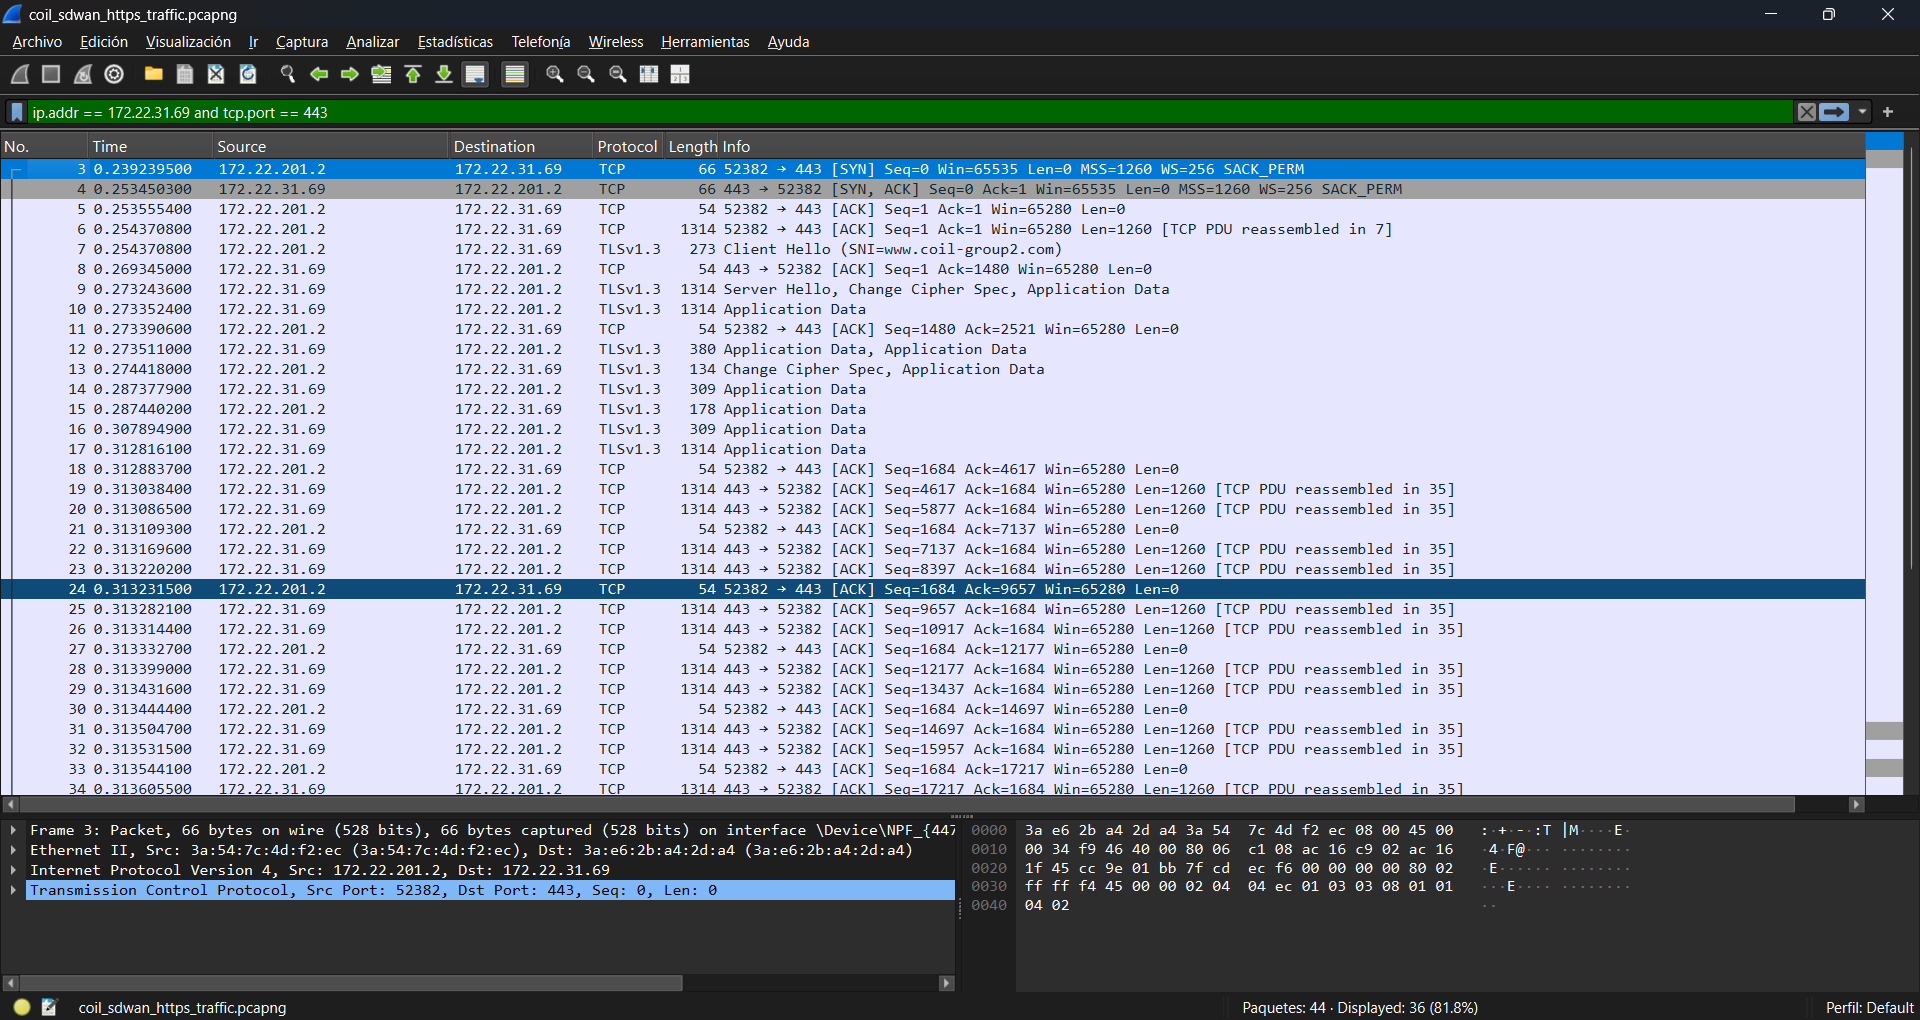
\includegraphics[width=0.94\textwidth]{figuras/wireshark_1_filtered_traffic.png}
    \caption{Wireshark packet list with the display filter \texttt{ip.addr == 172.22.31.69 and tcp.port == 443} applied, isolating all \num{36} frames (\qty{22785}{\byte} wire, \qty{0.4083}{\second} duration) of the HTTPS conversation between UniLlanos (\nolinkurl{172.22.201.2:52382}) and Seneca (\nolinkurl{172.22.31.69:443}).}
    \label{fig:ws_filtered}
\end{figure*}

To map the wire-level packet stream onto its protocol state transitions before examining individual dissection panes, Fig.~\ref{fig:tcp_tls_sequence} synthesizes the complete end-to-end packet sequence diagram across TCP handshake, TLS~1.3 record exchange, segmented HTTP/1.1 response delivery, and four-way termination. The subsections that follow corroborate each phase in Fig.~\ref{fig:tcp_tls_sequence} directly against the corresponding Wireshark captures (Figs.~\ref{fig:ws_handshake}--\ref{fig:ws_teardown}).

\begin{figure*}[htbp]
\centering
\resizebox{0.84\textwidth}{!}{%
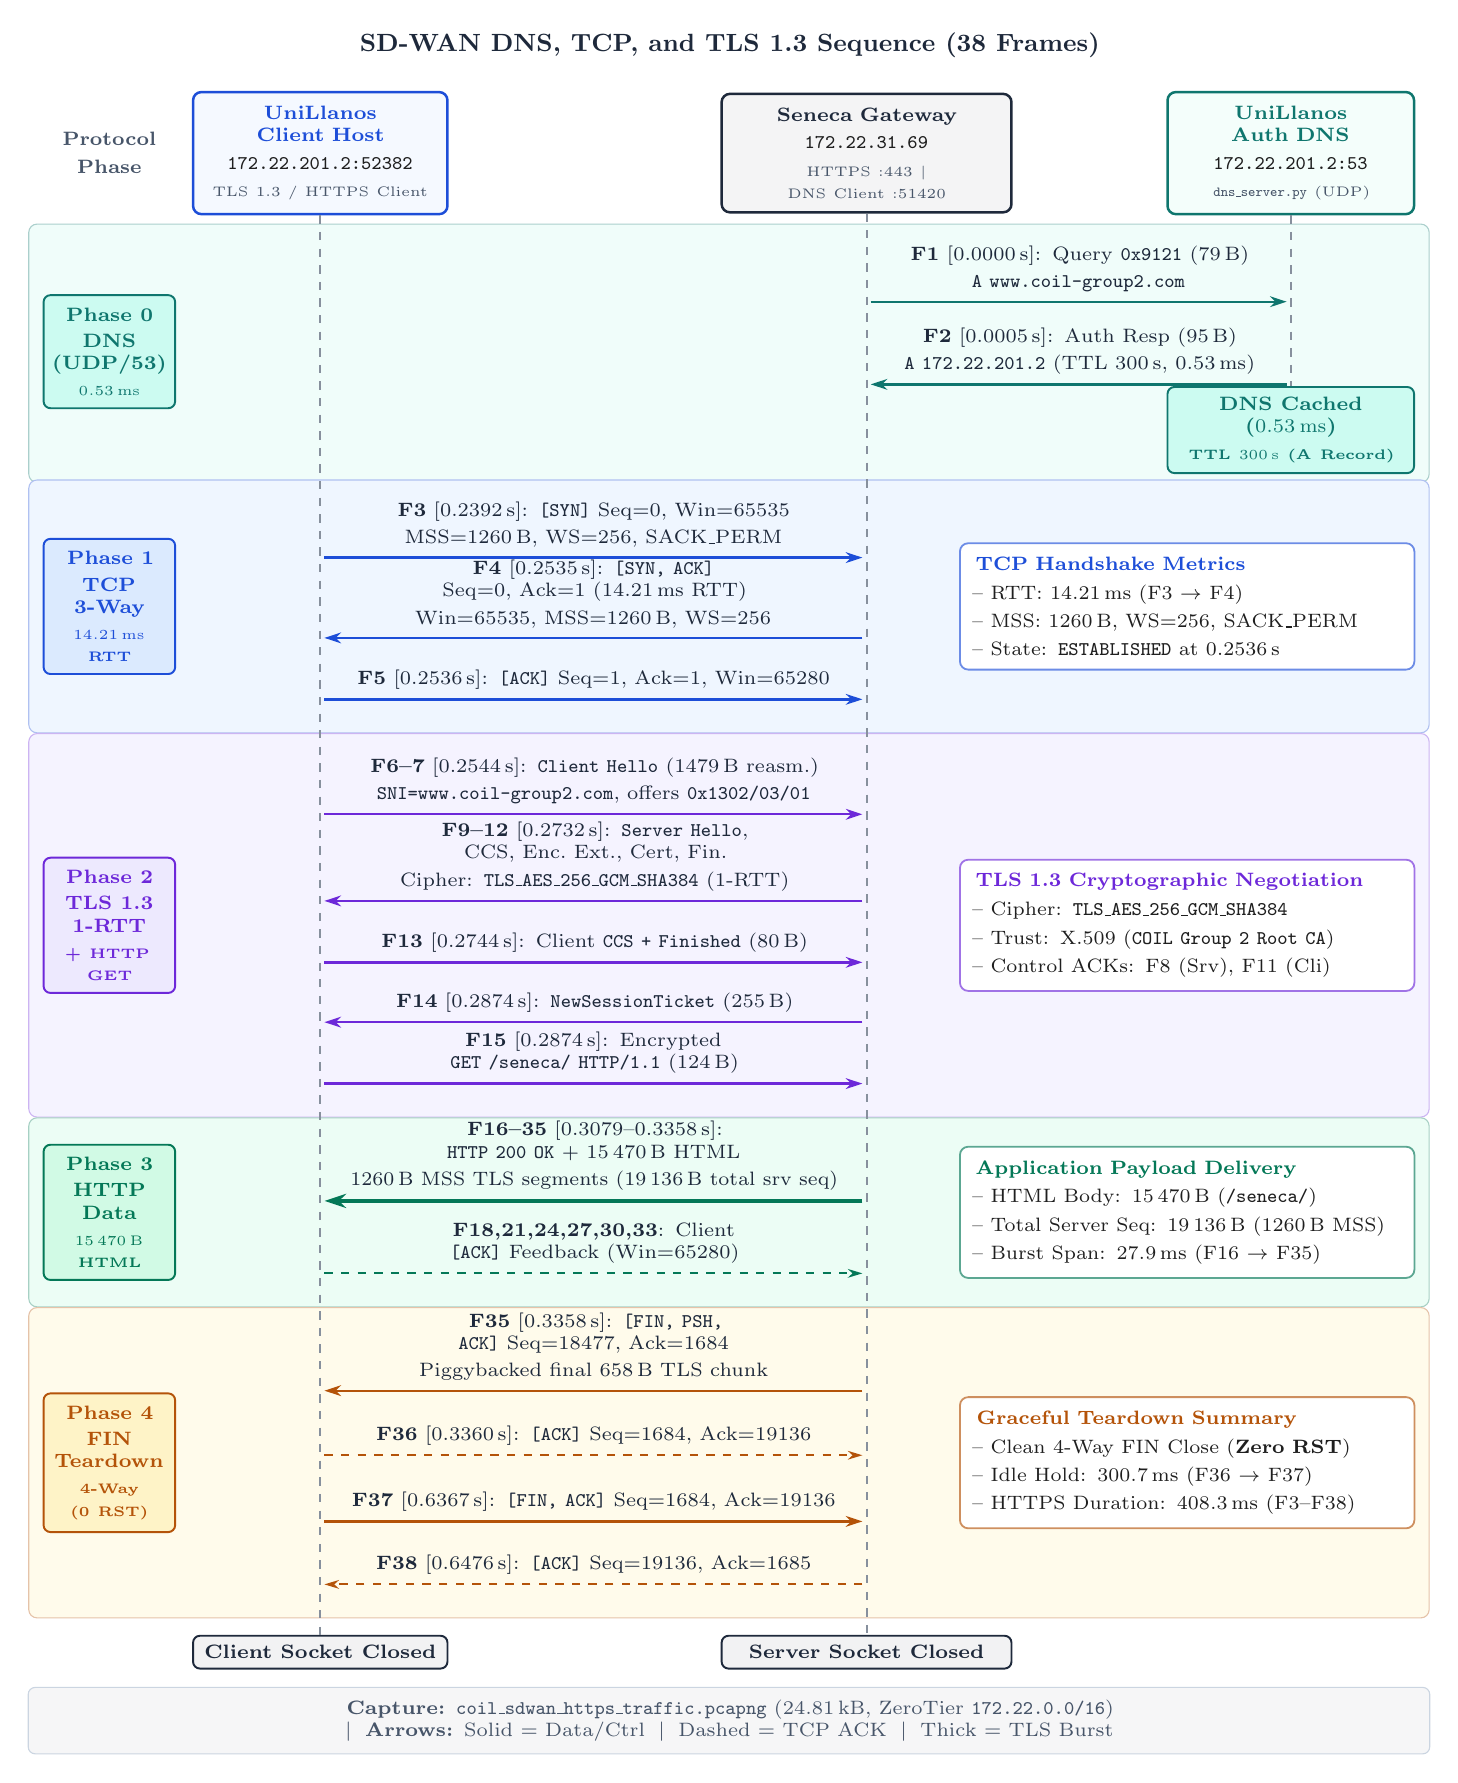
\begin{tikzpicture}[
    >=Stealth,
    every node/.style={font=\scriptsize, text=black!88},
    /utils/exec={
        \definecolor{figTwoSlate}{HTML}{1E293B}
        \definecolor{figTwoMuted}{HTML}{475569}
        \definecolor{figTwoRule}{HTML}{CBD5E1}
        \definecolor{figTwoDnsAccent}{HTML}{0F766E}
        \definecolor{figTwoDnsFill}{HTML}{F0FDFA}
        \definecolor{figTwoDnsBadge}{HTML}{CCFBF1}
        \definecolor{figTwoTcpAccent}{HTML}{1D4ED8}
        \definecolor{figTwoTcpFill}{HTML}{EFF6FF}
        \definecolor{figTwoTcpBadge}{HTML}{DBEAFE}
        \definecolor{figTwoTlsAccent}{HTML}{6D28D9}
        \definecolor{figTwoTlsFill}{HTML}{F5F3FF}
        \definecolor{figTwoTlsBadge}{HTML}{EDE9FE}
        \definecolor{figTwoDataAccent}{HTML}{047857}
        \definecolor{figTwoDataFill}{HTML}{ECFDF5}
        \definecolor{figTwoDataBadge}{HTML}{D1FAE5}
        \definecolor{figTwoFinAccent}{HTML}{B45309}
        \definecolor{figTwoFinFill}{HTML}{FFFBEB}
        \definecolor{figTwoFinBadge}{HTML}{FEF3C7}
    },
    endpoint/.style={
        rectangle, rounded corners=3pt, draw=figTwoSlate, fill=white,
        line width=0.9pt, align=center, inner xsep=4pt, inner ysep=5pt,
        minimum height=1.24cm, font=\scriptsize
    },
    endpoint_foot/.style={
        rectangle, rounded corners=2.5pt, draw=figTwoSlate, fill=figTwoSlate!6,
        line width=0.7pt, align=center, inner xsep=4pt, inner ysep=3.5pt,
        font=\scriptsize\bfseries, text=figTwoSlate
    },
    phase_badge/.style={
        rectangle, rounded corners=2.5pt, align=center,
        text width=1.46cm, inner xsep=3pt, inner ysep=4.5pt,
        line width=0.7pt, font=\scriptsize\bfseries
    },
    telemetry_card/.style={
        rectangle, rounded corners=3pt, align=left,
        text width=5.35cm, inner xsep=6pt, inner ysep=5pt,
        line width=0.65pt, fill=white, font=\scriptsize
    },
    msg_arrow/.style={
        -{Stealth[length=5pt 1.2, width'=0pt 0.65]},
        line width=0.85pt, shorten >=1.5pt, shorten <=1.5pt
    },
    msg_burst/.style={
        -{Stealth[length=6pt 1.2, width'=0pt 0.65]},
        line width=1.5pt, shorten >=1.5pt, shorten <=1.5pt
    },
    msg_ack/.style={
        -{Stealth[length=4.5pt 1.1, width'=0pt 0.6]},
        line width=0.7pt, dashed, shorten >=1.5pt, shorten <=1.5pt
    },
    msg_label/.style={
        anchor=south, yshift=2.2pt, align=center, inner sep=1pt,
        font=\scriptsize, text=figTwoSlate
    },
    lifeline/.style={
        dashed, line width=0.75pt, color=figTwoMuted!65
    }
]

\node[endpoint, text width=2.95cm, fill=figTwoTcpFill!65, draw=figTwoTcpAccent] (client_hdr) at (0,0) {%
    \textbf{\color{figTwoTcpAccent}UniLlanos Client Host}\\[2pt]
    \texttt{172.22.201.2:52382}\\[2pt]
    {\tiny\color{figTwoMuted}TLS 1.3 / HTTPS Client}%
};

\node[endpoint, text width=3.40cm, fill=figTwoSlate!5, draw=figTwoSlate, right=3.45cm of client_hdr] (server_hdr) {%
    \textbf{\color{figTwoSlate}Seneca Gateway}\\[2pt]
    \texttt{172.22.31.69}\\[2pt]
    {\tiny\color{figTwoMuted}HTTPS :443 \textbar{} DNS Client :51420}%
};

\node[endpoint, text width=2.85cm, fill=figTwoDnsFill!75, draw=figTwoDnsAccent, right=1.95cm of server_hdr] (dns_hdr) {%
    \textbf{\color{figTwoDnsAccent}UniLlanos Auth DNS}\\[2pt]
    \texttt{172.22.201.2:53}\\[2pt]
    {\tiny\color{figTwoMuted}\texttt{dns\_server.py} (UDP)}%
};

\node[left=0.22cm of client_hdr, minimum width=1.64cm, minimum height=1.24cm, inner sep=0pt] (phase_hdr_anchor) {};
\node[align=center, font=\scriptsize\bfseries, text=figTwoMuted] at (phase_hdr_anchor.center) {Protocol\\[2pt]Phase};

\coordinate (hdr_mid) at ($(phase_hdr_anchor.north west)!0.5!(dns_hdr.north east)$);
\node[anchor=south, font=\small\bfseries, text=figTwoSlate, inner sep=2pt] (fig_title) at ($(hdr_mid)+(0,0.42)$)
    {SD-WAN DNS, TCP, and TLS 1.3 Sequence (38 Frames)};

\coordinate (t_start) at (phase_hdr_anchor.south);

\coordinate (r_p0_top)  at ($(t_start)+(0,-0.38)$);
\coordinate (r_f1)      at ($(r_p0_top)+(0,-0.88)$);
\coordinate (r_f2)      at ($(r_f1)+(0,-1.05)$);
\coordinate (r_dns_end) at ($(r_f2)+(0,-0.58)$);
\coordinate (r_p0_bot)  at ($(r_dns_end)+(0,-0.52)$);

\coordinate (r_p1_top)  at ($(r_p0_bot)+(0,-0.22)$);
\coordinate (r_f3)      at ($(r_p1_top)+(0,-0.88)$);
\coordinate (r_f4)      at ($(r_f3)+(0,-1.02)$);
\coordinate (r_f5)      at ($(r_f4)+(0,-0.78)$);
\coordinate (r_p1_bot)  at ($(r_f5)+(0,-0.32)$);

\coordinate (r_p2_top)  at ($(r_p1_bot)+(0,-0.22)$);
\coordinate (r_f6)      at ($(r_p2_top)+(0,-0.92)$);
\coordinate (r_f9)      at ($(r_f6)+(0,-1.10)$);
\coordinate (r_f13)     at ($(r_f9)+(0,-0.78)$);
\coordinate (r_f14)     at ($(r_f13)+(0,-0.76)$);
\coordinate (r_f15)     at ($(r_f14)+(0,-0.78)$);
\coordinate (r_p2_bot)  at ($(r_f15)+(0,-0.32)$);

\coordinate (r_p3_top)  at ($(r_p2_bot)+(0,-0.22)$);
\coordinate (r_f16)     at ($(r_p3_top)+(0,-0.95)$);
\coordinate (r_f18)     at ($(r_f16)+(0,-0.92)$);
\coordinate (r_p3_bot)  at ($(r_f18)+(0,-0.32)$);

\coordinate (r_p4_top)  at ($(r_p3_bot)+(0,-0.22)$);
\coordinate (r_f35)     at ($(r_p4_top)+(0,-0.95)$);
\coordinate (r_f36)     at ($(r_f35)+(0,-0.82)$);
\coordinate (r_f37)     at ($(r_f36)+(0,-0.84)$);
\coordinate (r_f38)     at ($(r_f37)+(0,-0.80)$);
\coordinate (r_p4_bot)  at ($(r_f38)+(0,-0.32)$);

\coordinate (r_foot)    at ($(r_p4_bot)+(0,-0.32)$);

\node[endpoint_foot, anchor=north, text width=2.95cm] (client_foot) at (r_foot -| client_hdr.south) {Client Socket Closed};
\node[endpoint_foot, anchor=north, text width=3.40cm] (server_foot) at (r_foot -| server_hdr.south) {Server Socket Closed};

\node[rectangle, rounded corners=2.5pt, draw=figTwoDnsAccent, fill=figTwoDnsBadge,
      line width=0.7pt, align=center, text width=2.85cm, font=\scriptsize\bfseries, text=figTwoDnsAccent,
      inner xsep=4pt, inner ysep=3.5pt]
      (dns_done) at (r_dns_end -| dns_hdr.south)
      {DNS Cached (\qty{0.53}{\milli\second})\\[2pt]{\tiny TTL \qty{300}{\second} (A Record)}};

\draw[lifeline] (client_hdr.south) -- (client_foot.north);
\draw[lifeline] (server_hdr.south) -- (server_foot.north);
\draw[lifeline] (dns_hdr.south)    -- (dns_done.north);

\draw[msg_arrow, color=figTwoDnsAccent] (r_f1 -| server_hdr.south) -- (r_f1 -| dns_hdr.south)
    node[midway, msg_label, text width=4.85cm] {%
        \textbf{F1} [0.0000\,s]: Query \texttt{0x9121} (\qty{79}{\byte})\\[1.8pt]
        \texttt{A www.coil-group2.com}%
    };

\draw[msg_arrow, color=figTwoDnsAccent] (r_f2 -| dns_hdr.south) -- (r_f2 -| server_hdr.south)
    node[midway, msg_label, text width=4.85cm] {%
        \textbf{F2} [0.0005\,s]: Auth Resp (\qty{95}{\byte})\\[1.8pt]
        \texttt{A 172.22.201.2} (TTL \qty{300}{\second}, \qty{0.53}{\milli\second})%
    };

\draw[msg_arrow, color=figTwoTcpAccent] (r_f3 -| client_hdr.south) -- (r_f3 -| server_hdr.south)
    node[midway, msg_label, text width=6.15cm] {%
        \textbf{F3} [0.2392\,s]: \texttt{[SYN]} Seq=0, Win=65535\\[1.8pt]
        MSS=\qty{1260}{\byte}, WS=256, SACK\_PERM%
    };

\draw[msg_arrow, color=figTwoTcpAccent] (r_f4 -| server_hdr.south) -- (r_f4 -| client_hdr.south)
    node[midway, msg_label, text width=6.15cm] {%
        \textbf{F4} [0.2535\,s]: \texttt{[SYN, ACK]} Seq=0, Ack=1 (\qty{14.21}{\milli\second} RTT)\\[1.8pt]
        Win=65535, MSS=\qty{1260}{\byte}, WS=256%
    };

\draw[msg_arrow, color=figTwoTcpAccent] (r_f5 -| client_hdr.south) -- (r_f5 -| server_hdr.south)
    node[midway, msg_label, text width=6.15cm] {%
        \textbf{F5} [0.2536\,s]: \texttt{[ACK]} Seq=1, Ack=1, Win=65280%
    };

\draw[msg_arrow, color=figTwoTlsAccent] (r_f6 -| client_hdr.south) -- (r_f6 -| server_hdr.south)
    node[midway, msg_label, text width=6.15cm] {%
        \textbf{F6--7} [0.2544\,s]: \texttt{Client Hello} (\qty{1479}{\byte} reasm.)\\[1.8pt]
        \texttt{SNI=www.coil-group2.com}, offers \texttt{0x1302/03/01}%
    };

\draw[msg_arrow, color=figTwoTlsAccent] (r_f9 -| server_hdr.south) -- (r_f9 -| client_hdr.south)
    node[midway, msg_label, text width=6.15cm] {%
        \textbf{F9--12} [0.2732\,s]: \texttt{Server Hello}, CCS, Enc.\ Ext., Cert, Fin.\\[1.8pt]
        Cipher: \texttt{TLS\_AES\_256\_GCM\_SHA384} (1-RTT)%
    };

\draw[msg_arrow, color=figTwoTlsAccent] (r_f13 -| client_hdr.south) -- (r_f13 -| server_hdr.south)
    node[midway, msg_label, text width=6.15cm] {%
        \textbf{F13} [0.2744\,s]: Client \texttt{CCS + Finished} (\qty{80}{\byte})%
    };

\draw[msg_arrow, color=figTwoTlsAccent] (r_f14 -| server_hdr.south) -- (r_f14 -| client_hdr.south)
    node[midway, msg_label, text width=6.15cm] {%
        \textbf{F14} [0.2874\,s]: \texttt{NewSessionTicket} (\qty{255}{\byte})%
    };

\draw[msg_arrow, color=figTwoTlsAccent] (r_f15 -| client_hdr.south) -- (r_f15 -| server_hdr.south)
    node[midway, msg_label, text width=6.15cm] {%
        \textbf{F15} [0.2874\,s]: Encrypted \texttt{GET /seneca/ HTTP/1.1} (\qty{124}{\byte})%
    };

\draw[msg_burst, color=figTwoDataAccent] (r_f16 -| server_hdr.south) -- (r_f16 -| client_hdr.south)
    node[midway, msg_label, text width=6.15cm] {%
        \textbf{F16--35} [0.3079--0.3358\,s]: \texttt{HTTP 200 OK} + \qty{15470}{\byte} HTML\\[1.8pt]
        \qty{1260}{\byte} MSS TLS segments (\qty{19136}{\byte} total srv seq)%
    };

\draw[msg_ack, color=figTwoDataAccent] (r_f18 -| client_hdr.south) -- (r_f18 -| server_hdr.south)
    node[midway, msg_label, text width=6.15cm] {%
        \textbf{F18,21,24,27,30,33}: Client \texttt{[ACK]} Feedback (Win=65280)%
    };

\draw[msg_arrow, color=figTwoFinAccent] (r_f35 -| server_hdr.south) -- (r_f35 -| client_hdr.south)
    node[midway, msg_label, text width=6.15cm] {%
        \textbf{F35} [0.3358\,s]: \texttt{[FIN, PSH, ACK]} Seq=18477, Ack=1684\\[1.8pt]
        Piggybacked final \qty{658}{\byte} TLS chunk%
    };

\draw[msg_ack, color=figTwoFinAccent] (r_f36 -| client_hdr.south) -- (r_f36 -| server_hdr.south)
    node[midway, msg_label, text width=6.15cm] {%
        \textbf{F36} [0.3360\,s]: \texttt{[ACK]} Seq=1684, Ack=19136%
    };

\draw[msg_arrow, color=figTwoFinAccent] (r_f37 -| client_hdr.south) -- (r_f37 -| server_hdr.south)
    node[midway, msg_label, text width=6.15cm] {%
        \textbf{F37} [0.6367\,s]: \texttt{[FIN, ACK]} Seq=1684, Ack=19136%
    };

\draw[msg_ack, color=figTwoFinAccent] (r_f38 -| server_hdr.south) -- (r_f38 -| client_hdr.south)
    node[midway, msg_label, text width=6.15cm] {%
        \textbf{F38} [0.6476\,s]: \texttt{[ACK]} Seq=19136, Ack=1685%
    };

\coordinate (p0_mid) at ($(r_p0_top)!0.5!(r_p0_bot)$);
\coordinate (p1_mid) at ($(r_p1_top)!0.5!(r_p1_bot)$);
\coordinate (p2_mid) at ($(r_p2_top)!0.5!(r_p2_bot)$);
\coordinate (p3_mid) at ($(r_p3_top)!0.5!(r_p3_bot)$);
\coordinate (p4_mid) at ($(r_p4_top)!0.5!(r_p4_bot)$);

\node[phase_badge, fill=figTwoDnsBadge, draw=figTwoDnsAccent, text=figTwoDnsAccent] (b_p0) at (p0_mid)
    {Phase 0\\[1.5pt]DNS (UDP/53)\\[1.5pt]{\tiny\qty{0.53}{\milli\second}}};
\node[phase_badge, fill=figTwoTcpBadge, draw=figTwoTcpAccent, text=figTwoTcpAccent] (b_p1) at (p1_mid)
    {Phase 1\\[1.5pt]TCP 3-Way\\[1.5pt]{\tiny\qty{14.21}{\milli\second} RTT}};
\node[phase_badge, fill=figTwoTlsBadge, draw=figTwoTlsAccent, text=figTwoTlsAccent] (b_p2) at (p2_mid)
    {Phase 2\\[1.5pt]TLS 1.3 1-RTT\\[1.5pt]{\tiny + HTTP GET}};
\node[phase_badge, fill=figTwoDataBadge, draw=figTwoDataAccent, text=figTwoDataAccent] (b_p3) at (p3_mid)
    {Phase 3\\[1.5pt]HTTP Data\\[1.5pt]{\tiny\qty{15470}{\byte} HTML}};
\node[phase_badge, fill=figTwoFinBadge, draw=figTwoFinAccent, text=figTwoFinAccent] (b_p4) at (p4_mid)
    {Phase 4\\[1.5pt]FIN Teardown\\[1.5pt]{\tiny 4-Way (0 RST)}};

\node[telemetry_card, anchor=east, draw=figTwoTcpAccent!65] (card_p1) at (p1_mid -| dns_hdr.east) {%
    \textbf{\color{figTwoTcpAccent}TCP Handshake Metrics}\\[2.4pt]
    -- RTT: \qty{14.21}{\milli\second} (F3 $\to$ F4)\\[2.2pt]
    -- MSS: \qty{1260}{\byte}, WS=256, SACK\_PERM\\[2.2pt]
    -- State: \texttt{ESTABLISHED} at \qty{0.2536}{\second}%
};

\node[telemetry_card, anchor=east, draw=figTwoTlsAccent!65] (card_p2) at (p2_mid -| dns_hdr.east) {%
    \textbf{\color{figTwoTlsAccent}TLS 1.3 Cryptographic Negotiation}\\[2.4pt]
    -- Cipher: \texttt{TLS\_AES\_256\_GCM\_SHA384}\\[2.2pt]
    -- Trust: X.509 (\texttt{COIL Group 2 Root CA})\\[2.2pt]
    -- Control ACKs: F8 (Srv), F11 (Cli)%
};

\node[telemetry_card, anchor=east, draw=figTwoDataAccent!65] (card_p3) at (p3_mid -| dns_hdr.east) {%
    \textbf{\color{figTwoDataAccent}Application Payload Delivery}\\[2.4pt]
    -- HTML Body: \qty{15470}{\byte} (\texttt{/seneca/})\\[2.2pt]
    -- Total Server Seq: \qty{19136}{\byte} (\qty{1260}{\byte} MSS)\\[2.2pt]
    -- Burst Span: \qty{27.9}{\milli\second} (F16 $\to$ F35)%
};

\node[telemetry_card, anchor=east, draw=figTwoFinAccent!65] (card_p4) at (p4_mid -| dns_hdr.east) {%
    \textbf{\color{figTwoFinAccent}Graceful Teardown Summary}\\[2.4pt]
    -- Clean 4-Way FIN Close (\textbf{Zero RST})\\[2.2pt]
    -- Idle Hold: \qty{300.7}{\milli\second} (F36 $\to$ F37)\\[2.2pt]
    -- HTTPS Duration: \qty{408.3}{\milli\second} (F3--F38)%
};

\begin{scope}[on background layer]
    \node[fill=figTwoDnsFill, draw=figTwoDnsAccent!35, rounded corners=3pt, inner xsep=5pt, inner ysep=3pt,
          fit=(r_p0_top) (r_p0_bot) (b_p0) (dns_hdr.east |- r_p0_top) (dns_done)] (band_p0) {};
    \node[fill=figTwoTcpFill, draw=figTwoTcpAccent!35, rounded corners=3pt, inner xsep=5pt, inner ysep=3pt,
          fit=(r_p1_top) (r_p1_bot) (b_p1) (card_p1) (dns_hdr.east |- r_p1_top)] (band_p1) {};
    \node[fill=figTwoTlsFill, draw=figTwoTlsAccent!35, rounded corners=3pt, inner xsep=5pt, inner ysep=3pt,
          fit=(r_p2_top) (r_p2_bot) (b_p2) (card_p2) (dns_hdr.east |- r_p2_top)] (band_p2) {};
    \node[fill=figTwoDataFill, draw=figTwoDataAccent!35, rounded corners=3pt, inner xsep=5pt, inner ysep=3pt,
          fit=(r_p3_top) (r_p3_bot) (b_p3) (card_p3) (dns_hdr.east |- r_p3_top)] (band_p3) {};
    \node[fill=figTwoFinFill, draw=figTwoFinAccent!35, rounded corners=3pt, inner xsep=5pt, inner ysep=3pt,
          fit=(r_p4_top) (r_p4_bot) (b_p4) (card_p4) (dns_hdr.east |- r_p4_top)] (band_p4) {};
\end{scope}

\path let \p1 = (band_p4.west), \p2 = (band_p4.east),
          \n1 = {\x2 - \x1 - 12pt} in
    node[rectangle, rounded corners=2.5pt, draw=figTwoRule, fill=figTwoSlate!4,
         anchor=north, inner xsep=6pt, inner ysep=4.5pt, font=\scriptsize, text=figTwoMuted,
         text width=\n1, align=center] (legend_bar)
         at ($(band_p4.south |- client_foot.south)+(0,-0.22)$) {%
        \textbf{Capture:} \texttt{coil\_sdwan\_https\_traffic.pcapng} (\qty{24.81}{\kilo\byte}, ZeroTier \texttt{172.22.0.0/16})
        \;\textbar\;
        \textbf{Arrows:} Solid = Data/Ctrl \;\textbar\; Dashed = TCP ACK \;\textbar\; Thick = TLS Burst%
    };

\end{tikzpicture}%
}
\caption{End-to-end packet sequence diagram reconstructed from \texttt{coil\_sdwan\_https\_traffic.pcapng} (\qty{24.81}{\kilo\byte}), illustrating Phase~0 authoritative DNS resolution (Frames~1--2, \qty{0.53}{\milli\second}), Phase~1 TCP three-way handshake (Frames~3--5, \qty{14.21}{\milli\second} RTT, MSS~\qty{1260}{\byte}), Phase~2 TLS~1.3 1-RTT negotiation (\texttt{TLS\_AES\_256\_GCM\_SHA384}) and encrypted \texttt{GET /seneca/} request (Frames~6--15), Phase~3 application payload delivery (\qty{15470}{\byte} HTML across Frames~16--35), and Phase~4 graceful four-way FIN teardown (Frames~35--38, zero \texttt{RST}).}
\label{fig:tcp_tls_sequence}
\end{figure*}


\subsection{Initial TCP Three-Way Handshake and SD-WAN MSS Calibration}
\label{subsec:ws_handshake}

Reliable connection-oriented delivery begins with the RFC~9293 three-way handshake~\cite{rfc9293,kozierok2005} captured in Frames~3--5 and inspected in Fig.~\ref{fig:ws_handshake} (top left of the timeline in Fig.~\ref{fig:tcp_tls_sequence}):
\begin{enumerate}
    \item \textbf{Frame~3 (\qty{0.2392395}{\second}, \qty{66}{\byte} wire):} The UniLlanos client (\nolinkurl{172.22.201.2:52382}) transmits a \texttt{[SYN]} segment toward \nolinkurl{172.22.31.69:443} with relative \texttt{Seq=0}, initial receive window \texttt{Win=65535}, \texttt{Len=0}, and \qty{12}{\byte} of TCP options declaring \texttt{MSS=1260}, Window Scale \texttt{WS=256} (shift count~\num{8}), and Selective Acknowledgment Permitted (\texttt{SACK\_PERM}).
    \item \textbf{Frame~4 (\qty{0.2534503}{\second}, \qty{66}{\byte} wire):} The Seneca gateway (\nolinkurl{172.22.31.69:443}) responds with \texttt{[SYN, ACK]}, setting relative \texttt{Seq=0}, \texttt{Ack=1} (consuming the client's virtual \texttt{SYN} sequence octet), \texttt{Win=65535}, and symmetric options \texttt{MSS=1260}, \texttt{WS=256}, and \texttt{SACK\_PERM}. The timestamp delta between Frame~3 and Frame~4 yields an empirical SD-WAN handshake Round-Trip Time (RTT) of \qty{14.21}{\milli\second} (\qty{0.0142108}{\second}).
    \item \textbf{Frame~5 (\qty{0.2535554}{\second}, \qty{54}{\byte} wire):} The client completes state synchronization with a pure \texttt{[ACK]} (\texttt{Seq=1}, \texttt{Ack=1}, \texttt{Len=0}), transitioning both sockets to \texttt{ESTABLISHED}. Because window scaling is now active, the nominal 16-bit header field value of \num{255} scales by \texttt{WS=256} to advertise a calculated receive window of \texttt{Win=65280} bytes ($255 \times 256 = \qty{65280}{\byte}$).
\end{enumerate}

Crucially, the negotiated \texttt{MSS=1260} observed in Fig.~\ref{fig:ws_handshake} directly reflects the underlying ZeroTier SD-WAN link geometry~\cite{tanenbaum2021}. Subtracting the standard \qty{20}{\byte} IPv4 header and \qty{20}{\byte} base TCP header (\qty{40}{\byte} total protocol overhead) from the ZeroTier virtual interface MTU of \qty{1300}{\byte} constrains maximum TCP payload per segment to $1300 - 40 = \qty{1260}{\byte}$, preventing outer UDP overlay fragmentation on physical WAN links.

\begin{figure*}[t]
    \centering
    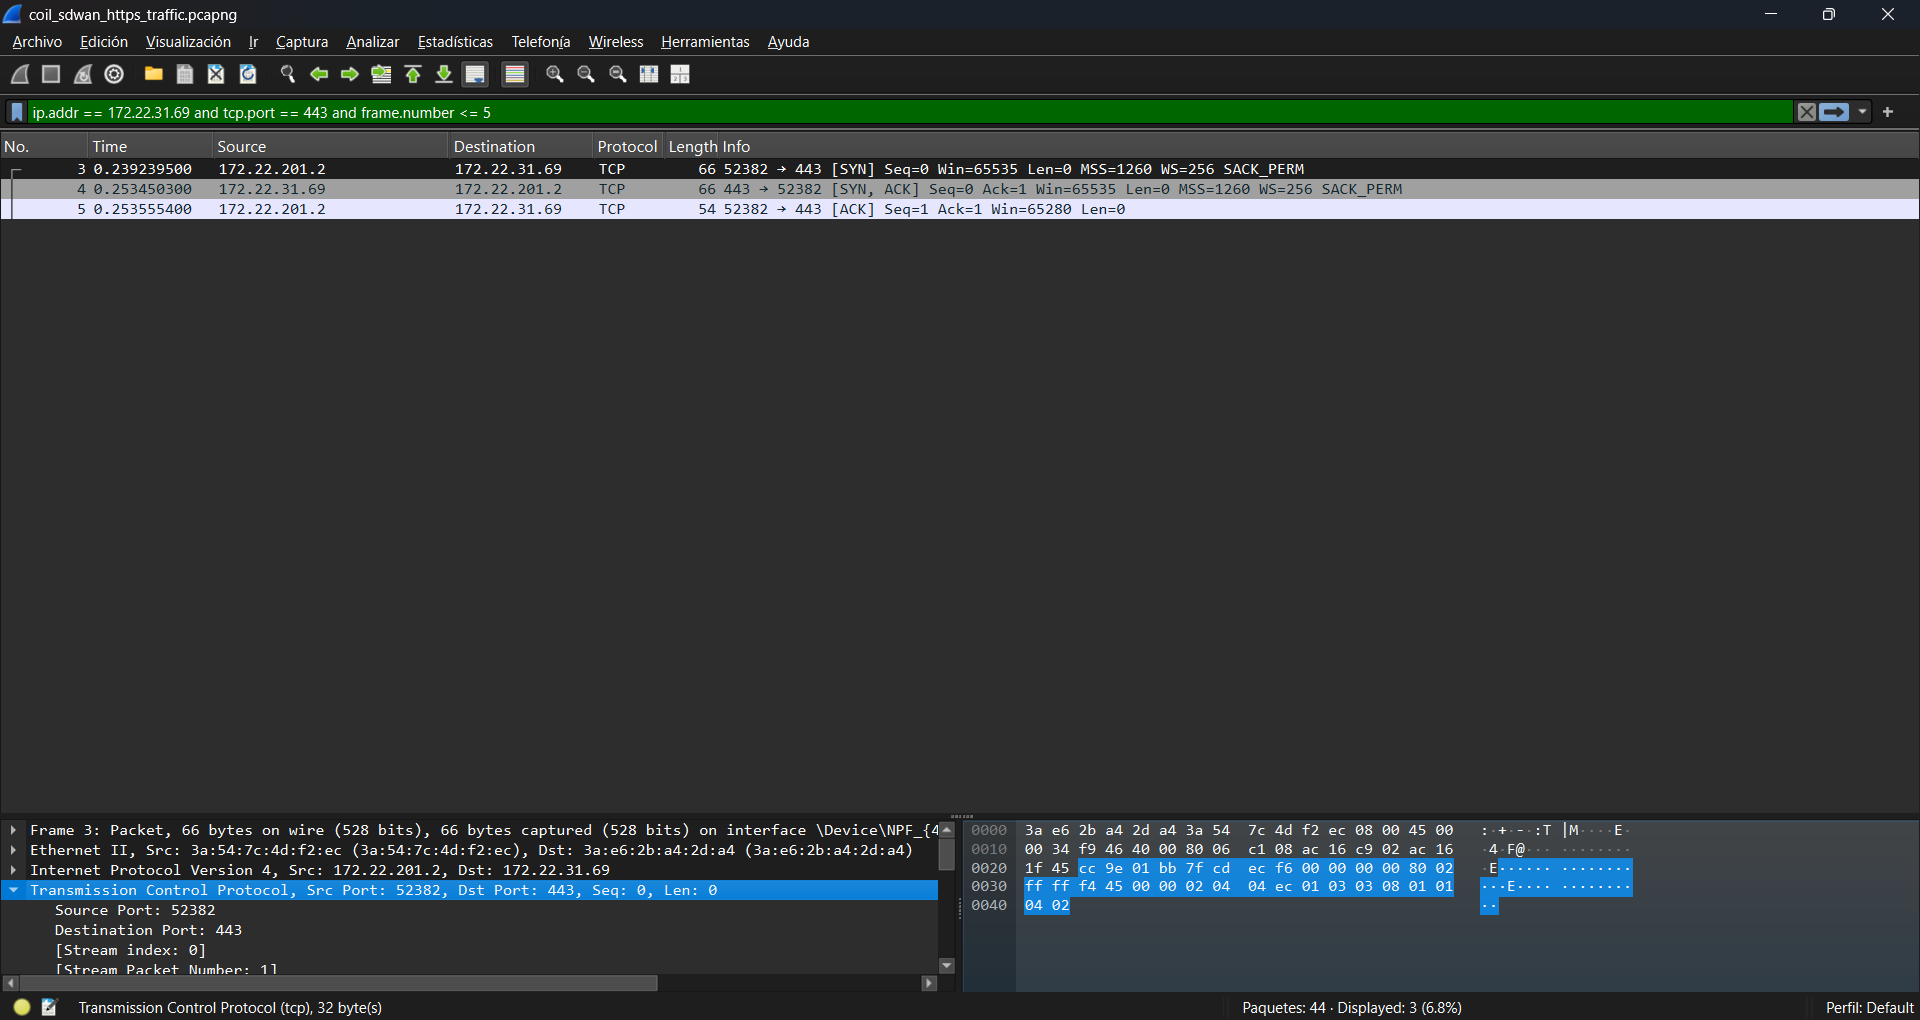
\includegraphics[width=0.94\textwidth]{figuras/wireshark_2_tcp_handshake.png}
    \caption{Wireshark packet details for the initial TCP three-way handshake (Frames~3--5), confirming \texttt{MSS=1260} matching the \qty{1300}{\byte} ZeroTier MTU minus \qty{40}{\byte} IPv4/TCP headers, \texttt{WS=256} scaling to \texttt{Win=65280}, \texttt{SACK\_PERM}, and a \qty{14.21}{\milli\second} handshake RTT.}
    \label{fig:ws_handshake}
\end{figure*}

\subsection{TLS 1.3 Cryptographic Handshake and Encrypted HTTP/1.1 Payload Transfer}
\label{subsec:ws_tls}

Immediately following TCP synchronization, Frames~6--35 execute the RFC~8446 TLS~1.3 handshake and encrypted application-layer exchange~\cite{rfc8446}, illustrated in Fig.~\ref{fig:ws_tls} and traced in Fig.~\ref{fig:tcp_tls_sequence}:
\begin{itemize}
    \item \textbf{Segmented Client Hello (Frames~6--7, \qty{0.2543708}{\second}):} The client initiates cryptographic negotiation with a \texttt{Client Hello} carrying Server Name Indication (\texttt{SNI=www.coil-group2.com}), \texttt{supported\_versions} (\texttt{TLS 1.3}), three AEAD cipher suites---\texttt{0x1302} (\nolinkurl{TLS_AES_256_GCM_SHA384}), \texttt{0x1303} (\nolinkurl{TLS_CHACHA20_POLY1305_SHA256}), and \texttt{0x1301} (\nolinkurl{TLS_AES_128_GCM_SHA256})---and an extended \texttt{key\_share} payload offering hybrid post-quantum \texttt{X25519MLKEM768} alongside \texttt{x25519}. Because the resulting \qty{1479}{\byte} TCP payload exceeds the \qty{1260}{\byte} MSS, TCP segments the message into Frame~6 (\qty{1260}{\byte} payload) and Frame~7 (\qty{219}{\byte} payload), which Wireshark reassembles ($1260 + 219 = \qty{1479}{\byte}$) into the complete \texttt{Client Hello} record.
    \item \textbf{Single-RTT Server Flight (Frames~9--12, \qty{0.2732436}{\second}):} After acknowledging Frame~7 (\texttt{Ack=1480} in Frame~8), the server responds in a single round trip across Frames~9--12 (\qty{2900}{\byte} TLS handshake flight). Frame~9 begins with \texttt{Server Hello}, selecting cipher suite \texttt{0x1302} (\nolinkurl{TLS_AES_256_GCM_SHA384}) and \texttt{x25519} key agreement, followed immediately by a middlebox-compatibility \texttt{Change Cipher Spec} record and encrypted handshake records spanning Frames~9, 10, and 12 (\texttt{Encrypted Extensions}, the X.509 certificate chain anchored to \texttt{COIL Group 2 Root CA}, \texttt{CertificateVerify}, and \texttt{Finished}).
    \item \textbf{Encrypted HTTP/1.1 Transaction (Frames~13--35, \qty{0.2744180}{\second}--\qty{0.3358339}{\second}):} At \qty{0.2744180}{\second} (Frame~13, \qty{80}{\byte} TCP payload), the client emits \texttt{Change Cipher Spec} plus its encrypted \texttt{Finished} message; the server issues post-handshake session tickets in Frames~14 and~16 (\qty{255}{\byte} TCP payload each). In Frame~15 (\qty{0.2874402}{\second}, \qty{178}{\byte} wire), the client transmits the encrypted HTTP \texttt{GET /seneca/} request inside a \qty{124}{\byte} TLS application-data payload (\texttt{Seq=1560..1683}). The server then delivers the HTTP \texttt{200 OK} headers and the full \qty{15470}{\byte} HTML document (\qty{15734}{\byte} decrypted HTTP bytes total) across Frames~17--35. Consistent with the negotiated \texttt{MSS=1260}, bulk server segments (Frames~17, 19--20, 22--23, 25--26, 28--29, 31--32, and~34) each carry exactly \qty{1260}{\byte} of encrypted payload (\qty{1314}{\byte} wire), while the final application record in Frame~35 (\qty{658}{\byte} payload) advances the server's relative sequence space to \texttt{Seq=19136}.
\end{itemize}

Because all HTTP headers and HTML markup after \texttt{Server Hello} and client \texttt{Finished} appear strictly as opaque TLS~1.3 \texttt{Application Data} in Fig.~\ref{fig:ws_tls}, passive observers on either the underlay network or the virtual broadcast domain cannot recover payload content or tamper with responses without failing AEAD authentication~\cite{rfc8446}.

\begin{figure*}[t]
    \centering
    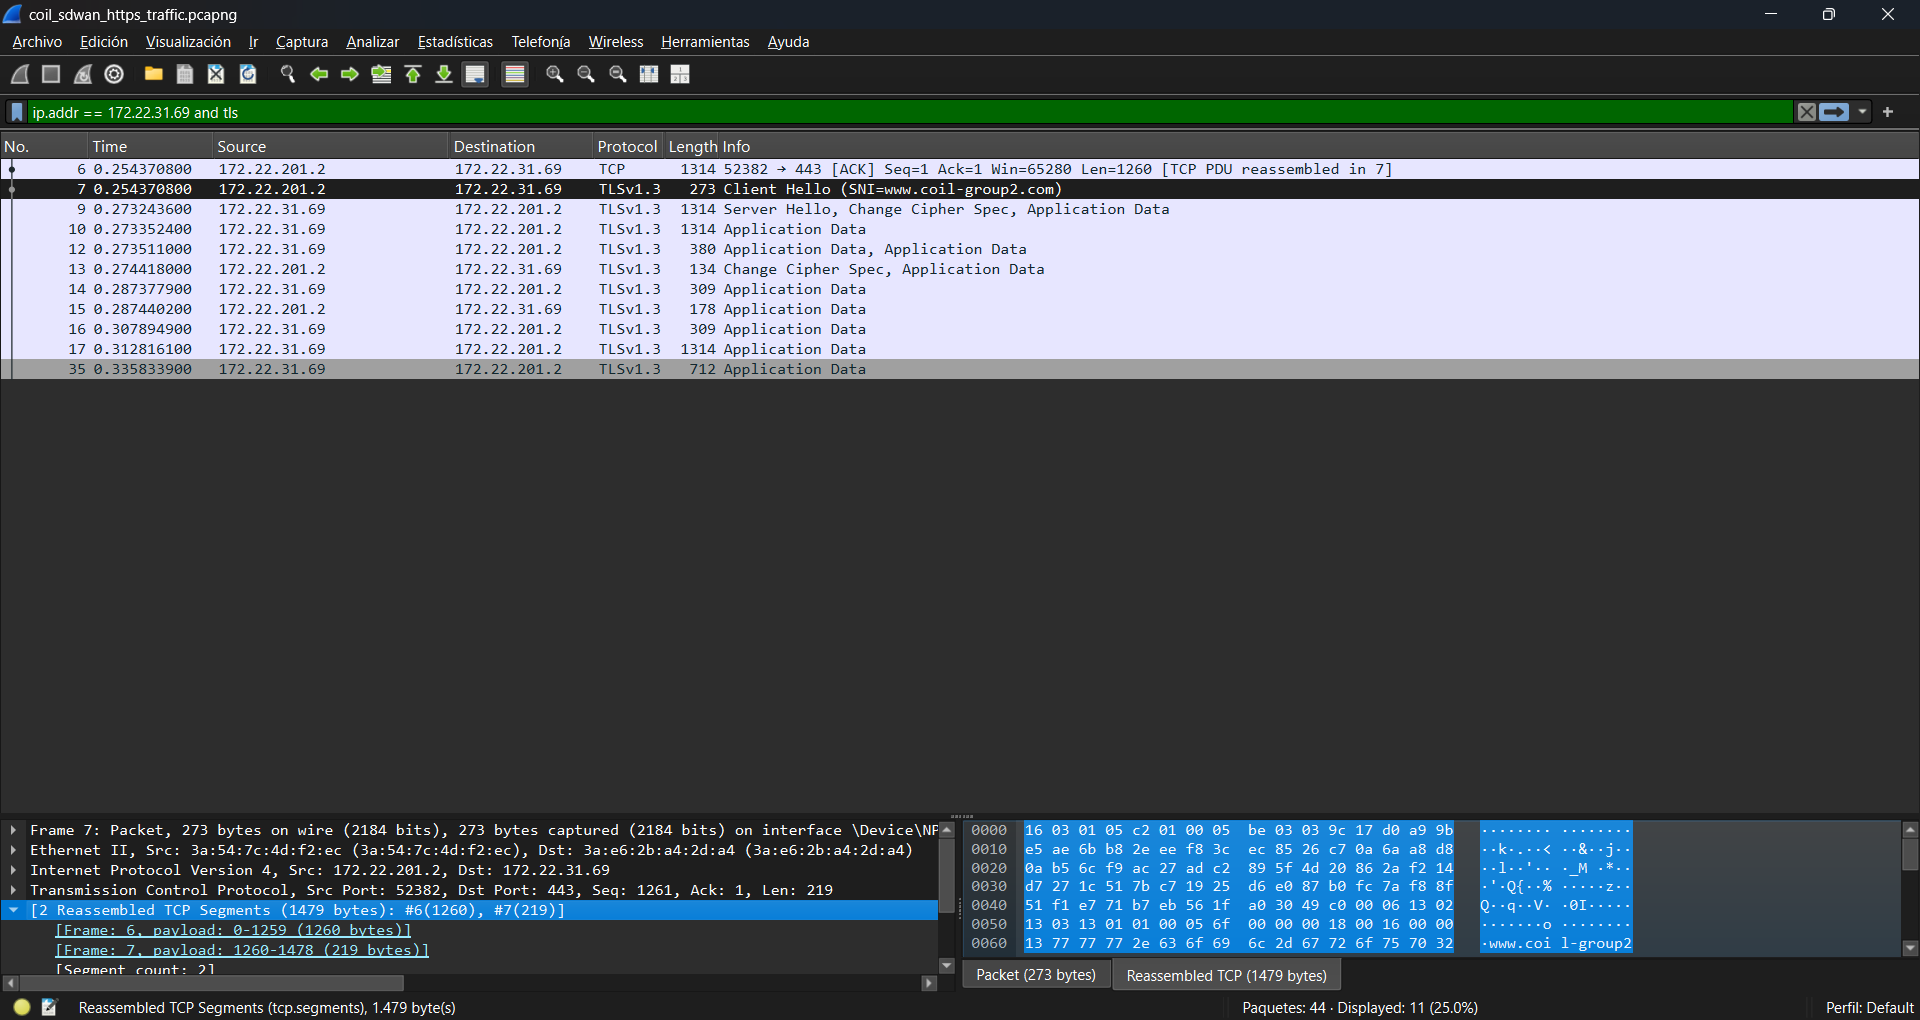
\includegraphics[width=0.94\textwidth]{figuras/wireshark_3_tls_data_exchange.png}
    \caption{Wireshark inspection of the TLS~1.3 cryptographic handshake and encrypted HTTP/1.1 payload exchange (Frames~6--35), showing reassembled \texttt{Client Hello} (\texttt{SNI=www.coil-group2.com}), 1-RTT \texttt{Server Hello} selecting \texttt{TLS\_AES\_256\_GCM\_SHA384} (\texttt{0x1302}), and \qty{1260}{\byte}-MSS segmented delivery of the \qty{15470}{\byte} Seneca HTML response.}
    \label{fig:ws_tls}
\end{figure*}

\subsection{Graceful TCP Connection Teardown}
\label{subsec:ws_teardown}

Once the Seneca HTML payload is transmitted, the server closes the connection cleanly in accordance with HTTP/1.1 \texttt{Connection: close} header semantics and RFC~9293 finite-state termination~\cite{rfc9293,kozierok2005}. Fig.~\ref{fig:ws_teardown} highlights the final four teardown frames (Frames~35--38, corresponding to the bottom phase of Fig.~\ref{fig:tcp_tls_sequence}):
\begin{enumerate}
    \item \textbf{Frame~35 (\qty{0.3358339}{\second}, \qty{712}{\byte} wire):} The server piggybacks \texttt{[FIN, PSH, ACK]} onto the concluding \qty{658}{\byte} encrypted payload segment (\texttt{Seq=18477}, \texttt{Ack=1684}, \texttt{Len=658}), incrementing its cumulative sequence boundary by $658 + 1 = 659$ to \num{19136}.
    \item \textbf{Frame~36 (\qty{0.3359537}{\second}, \qty{54}{\byte} wire):} Within \qty{0.1198}{\milli\second}, the client transmits \texttt{[ACK]} (\texttt{Seq=1684}, \texttt{Ack=19136}, \texttt{Len=0}), acknowledging both the trailing payload bytes and the server's \texttt{FIN} flag to close the server-to-client half-channel.
    \item \textbf{Frame~37 (\qty{0.6367030}{\second}, \qty{54}{\byte} wire):} Upon completing local socket shutdown, the client issues \texttt{[FIN, ACK]} (\texttt{Seq=1684}, \texttt{Ack=19136}, \texttt{Len=0}) to close its own transmit half-channel.
    \item \textbf{Frame~38 (\qty{0.6475791}{\second}, \qty{54}{\byte} wire):} The server confirms termination with \texttt{[ACK]} (\texttt{Seq=19136}, \texttt{Ack=1685}, \texttt{Len=0}), cleanly retiring the session at \qty{0.4083}{\second} elapsed stream time.
\end{enumerate}

Verification against the display filter \texttt{tcp.flags.reset == 1} confirms \textbf{zero \texttt{RST} flags} across the entire capture file. The absence of forced resets proves that both TLS~1.3 session closure and HTTP/1.1 socket release operated deterministically without protocol errors or premature peer aborts.

\begin{figure*}[t]
    \centering
    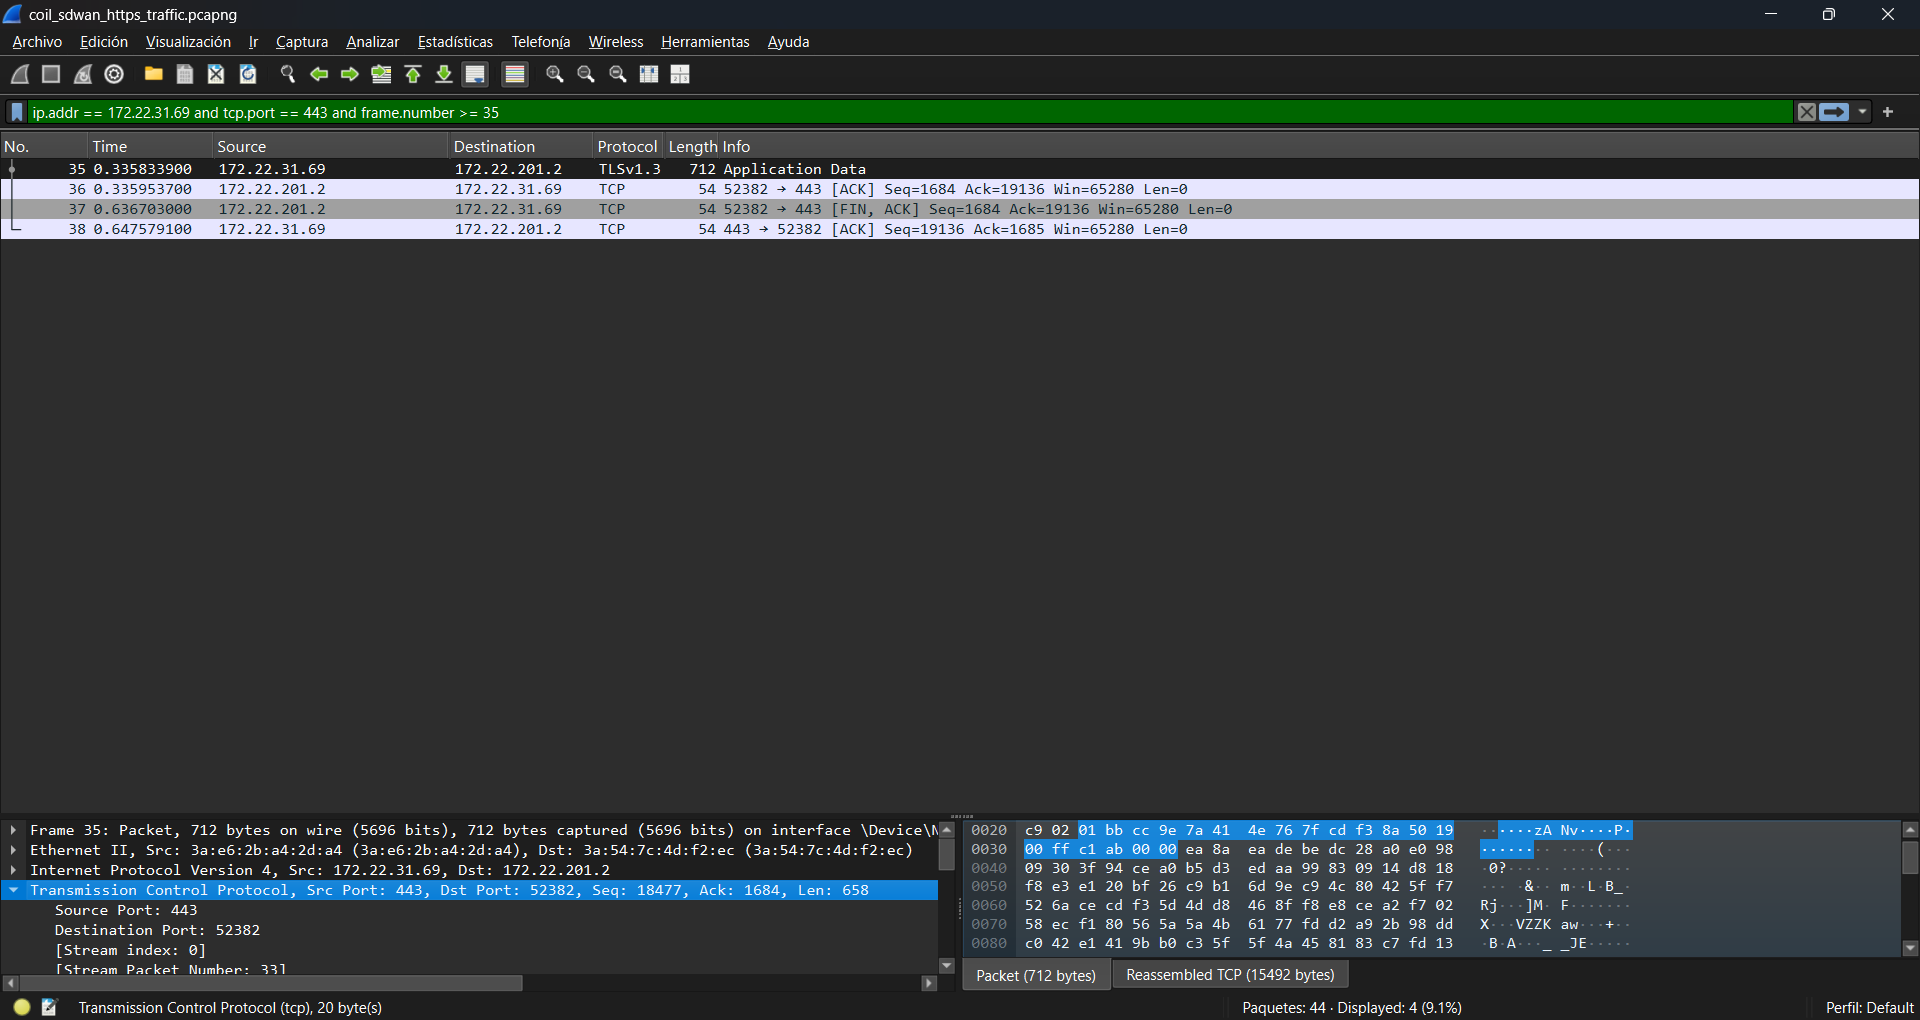
\includegraphics[width=0.94\textwidth]{figuras/wireshark_4_tcp_teardown.png}
    \caption{Wireshark inspection of the clean four-way TCP connection teardown (Frames~35--38), showing server \texttt{[FIN, PSH, ACK]} (\texttt{Seq=18477, Ack=1684, Len=658}), client \texttt{[ACK]} (\texttt{Ack=19136}), client \texttt{[FIN, ACK]}, and final server \texttt{[ACK]} (\texttt{Ack=1685}) with zero \texttt{RST} packets.}
    \label{fig:ws_teardown}
\end{figure*}

\section{Step-by-Step Implementation Manuals}
\label{sec:manuals}

Rubric Section~IV (\qty{50}{\percent} of the total evaluation) mandates four reproducible operational manuals accompanied by complete institutional source code in Appendices~\ref{app:unillanos_html}--\ref{app:pki_scripts}. To avoid duplication with the member inventory in Rubric Section~I, this section details Manual~1 (\qty{10}{\percent}: ZeroTier SD-WAN provisioning, static IP pinning, and MTU/MSS tuning) and Manual~2 (\qty{10}{\percent}: multi-tenant HTTPS/HTTP server engineering, OS persistence, and intranet UI walkthrough), while the companion PKI trust and authoritative DNS manuals (Manuals~3 and~4, \qty{15}{\percent} each) follow in the next section.

\subsection{Manual 1 (10\%): ZeroTier SD-WAN Network Creation and Configuration}
\label{subsec:manual1_sdwan}

ZeroTier decouples its cryptographic control plane (Virtual Layer~1, VL1) from a flat virtual Ethernet switching fabric (Virtual Layer~2, VL2), encapsulating Ethernet frames inside encrypted UDP port~9993 tunnels across heterogeneous NAT and ISP boundaries~\cite{zerotier2024,tanenbaum2021,kurose2017}. Provisioning the bilateral COIL overlay proceeds through five deterministic stages.

\subsubsection{Network Creation and Private Access Control}
Log in to ZeroTier Central (\nolinkurl{https://my.zerotier.com}) and click \textbf{Create A Network} to allocate a globally unique 64-bit (16-hexadecimal-character) Network ID, assigned to this project as \texttt{abfd31bd47affa39}. Under \textbf{Settings} $\rightarrow$ \textbf{Basics}, enter the descriptive network name \textit{COIL Group 2 SD-WAN - UniLlanos \& Seneca} and set \textbf{Access Control} to \textbf{Private}. Enforcing \textit{Private} admission ensures that the controller drops VL2 traffic from any 40-bit ZeroTier Node ID whose cryptographic identity has not been explicitly authorized~\cite{zerotier2024}.

\subsubsection{Managed Routing, IPv4/IPv6 Pools, Multicast, and DNS Push}
Under \textbf{Settings} $\rightarrow$ \textbf{Advanced}, define the IPv4 addressing plan and link-layer controls shown in Fig.~\ref{fig:zerotier_settings}:
\begin{itemize}
    \item \textbf{Managed Routes:} Add \nolinkurl{172.22.0.0/16} with a blank \texttt{Via} field (marking it as an on-link \texttt{LAN} route) so every authorized member routes inter-institutional traffic directly across the virtual switch without an external gateway hop.
    \item \textbf{IPv4 Auto-Assign:} Enable \textbf{Easy} mode and select the \nolinkurl{172.22.*.*} block (\nolinkurl{172.22.0.1}--\nolinkurl{172.22.255.254}), isolating the SD-WAN from overlapping residential \nolinkurl{192.168.x.x} and campus \nolinkurl{10.x.x.x} subnets.
    \item \textbf{Multicast \& Broadcast Policy:} Set \textbf{Multicast Recipient Limit} to \num{32} and check \textbf{Enable Broadcast}, guaranteeing standard ARP discovery within \nolinkurl{172.22.0.0/16} while bounding WAN multicast replication overhead.
\end{itemize}

\begin{figure*}[t]
\centering
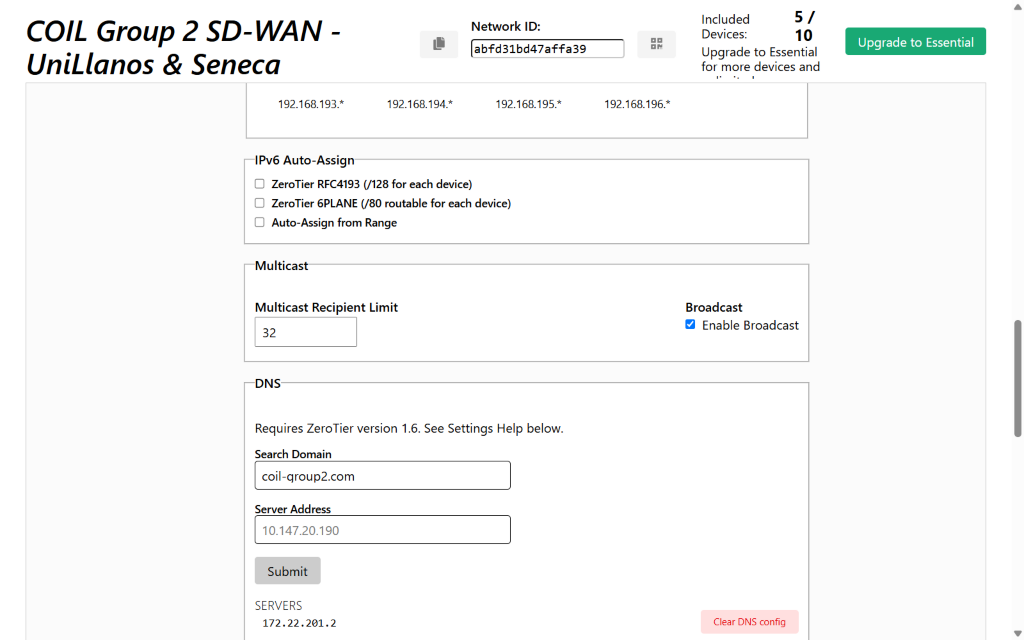
\includegraphics[width=0.84\textwidth]{figuras/zerotier_settings_dns_fresh.png}
\caption{ZeroTier Central advanced configuration console for Network ID \texttt{abfd31bd47affa39}, illustrating the IPv4 Easy Auto-Assign grid edge, disabled IPv6 auto-assignment checkboxes, Multicast Recipient Limit (\num{32}) with Broadcast enabled, and the ZeroTier~1.6+ authoritative DNS push configuration (\texttt{coil-group2.com} served by \texttt{172.22.201.2}).}
\label{fig:zerotier_settings}
\end{figure*}

As captured in Fig.~\ref{fig:zerotier_settings}, every panel in the ZeroTier Central settings view plays an explicit engineering role:
\begin{enumerate}
    \item \textbf{Top Network Header:} Displays the title \textit{COIL Group 2 SD-WAN - UniLlanos \& Seneca}, clipboard and QR-code enrollment shortcuts for \texttt{abfd31bd47affa39}, the free-tier quota counter (\textit{Included Devices: 5 / 10}), and the plan upgrade banner.
    \item \textbf{IPv4 Auto-Assign Grid:} Only the bottom row (\nolinkurl{192.168.193.*}--\nolinkurl{192.168.196.*}) falls within the scrolled viewport edge, above which the active \nolinkurl{172.22.*.*} subnet allocation is selected.
    \item \textbf{IPv6 Auto-Assign Panel:} All three checkboxes---\textit{ZeroTier RFC4193 (/128 for each device)}, \textit{ZeroTier 6PLANE (/80 routable for each device)}, and \textit{Auto-Assign from Range}---remain intentionally unchecked so Windows and Android hosts keep IPv4-only SD-WAN routing, eliminating extraneous ICMPv6 neighbor discovery and \texttt{AAAA} DNS queries in packet captures.
    \item \textbf{Multicast Panel:} Displays \textbf{Multicast Recipient Limit} fixed at \num{32} alongside the checked \textbf{Broadcast} (\textit{Enable Broadcast}) box.
    \item \textbf{DNS Panel:} Indicates the \textit{Requires ZeroTier version 1.6} prerequisite, specifies \textbf{Search Domain} as \nolinkurl{coil-group2.com}, displays the \textbf{Server Address} input field (placeholder \nolinkurl{10.147.20.190}) and \textbf{Submit} button, and confirms \nolinkurl{172.22.201.2} under \textbf{SERVERS} (with a \textbf{Clear DNS config} reset control) to push authoritative DNS automatically to enrolled nodes (detailed further in Manual~4).
\end{enumerate}

\subsubsection{Client Installation and Elevated Network Enrollment}
Deploy the ZeroTier One client across all five institutional and student endpoints---Miguel's UniLlanos web server laptop, the simulated Seneca gateway (\texttt{miguel2}), Luis Alejandro's Windows workstation, and both Android smartphones:
\begin{enumerate}
    \item \textbf{Windows Desktop and Server Nodes (\texttt{v1.16.2}):} Install the \texttt{x86\_64} ZeroTier One service silently from PowerShell using \texttt{winget}, as shown in Listing~\ref{lst:zt_join}.
    \item \textbf{Android Mobile Nodes (\texttt{v1.16.0}):} Install ZeroTier One (\texttt{arm64}) from Google Play, tap \textbf{Add Network}, and enroll \texttt{abfd31bd47affa39} (or scan the header QR code).
    \item \textbf{Elevated Windows CLI Join:} On Windows, the local ZeroTier daemon secures its IPC token (\texttt{C:\textbackslash{}ProgramData\textbackslash{}\allowbreak ZeroTier\textbackslash{}One\textbackslash{}\allowbreak authtoken.secret}) with Administrator-only permissions; non-elevated terminals exit with an unreadable-token error. Open an elevated Administrator PowerShell session and execute Listing~\ref{lst:zt_join} on each Windows host.
\end{enumerate}

\begin{lstlisting}[caption={Windows ZeroTier One installation, elevated join, and MTU tuning commands.},label={lst:zt_join}]
# 1. Install ZeroTier One (v1.16.2 x86_64) via winget
winget install zerotier.zerotierone --silent `
  --accept-package-agreements --accept-source-agreements

# 2. Join SD-WAN from elevated Administrator PowerShell
zerotier-cli join abfd31bd47affa39
zerotier-cli listnetworks

# 3. Clamp virtual interface MTU to 1300 B (MSS = 1260 B)
Set-NetIPInterface `
  -InterfaceAlias "ZeroTier One [abfd31bd47affa39]" `
  -AddressFamily IPv4 -NlMtuBytes 1300
netsh interface ipv4 show subinterfaces
\end{lstlisting}

\subsubsection{Device Authorization, Role Labeling, and Static IP Pinning}
In the ZeroTier Central \textbf{Members} table, verify each incoming Node ID against its local \texttt{zerotier-cli info} output, check the \textbf{Auth} box, and enforce the rubric's descriptive \textit{Name + Website} naming convention so evaluators can immediately distinguish servers from student clients. Pin static virtual IPv4 addresses by removing ephemeral dynamic leases and assigning deterministic addresses within \nolinkurl{172.22.0.0/16}: \nolinkurl{172.22.201.2} for the UniLlanos web/DNS server, \nolinkurl{172.22.31.69} for the Seneca partner gateway, and \nolinkurl{172.22.100.11} for Luis Alejandro's Windows workstation (complemented by Android client leases). Rather than duplicating the complete five-node registry here, Table~\ref{tab:zerotier_members} and Fig.~\ref{fig:sdwan_topology} in Rubric Section~I provide the authoritative member inventory, firmware versions (\texttt{v1.16.2} on Windows and \texttt{v1.16.0} on Android), physical endpoints, and mesh topology.

\subsubsection{Interface MTU Tuning for Fragmentation-Free Transport}
ZeroTier's default virtual Ethernet MTU of \qty{2800}{\byte} exceeds standard physical Ethernet (\qty{1500}{\byte}), PPPoE DSL (\qty{1492}{\byte}), and mobile cellular LTE/5G bearer MTUs (\qtyrange{1400}{1420}{\byte}) once VL1 UDP/cryptographic encapsulation headers are prepended~\cite{zerotier2024,tanenbaum2021}. Left untuned, large TLS certificate chains trigger outer-UDP fragmentation and packet loss across strict cellular NATs. Executing \texttt{Set-NetIPInterface} in Listing~\ref{lst:zt_join} constrains the ZeroTier virtual adapter to an IPv4 MTU of \qty{1300}{\byte}, verified via \texttt{netsh} on both the UniLlanos host and the Seneca gateway. Subtracting the mandatory \qty{20}{\byte} IPv4 header and \qty{20}{\byte} standard TCP header yields an exact Maximum Segment Size of $\text{MSS} = 1300 - 40 = \qty{1260}{\byte}$, matching the TCP three-way handshake negotiation observed in Rubric Section~III's Wireshark trace.

\subsection{Manual 2 (10\%): Multi-Tenant Web Server Creation and Intranet UI Deployment}
\label{subsec:manual2_web}

Both institutions must host cultural intranets accessible by IPv4 address and domain URL over TLS-encrypted HTTPS. Rather than relying on separate web engines, COIL Group~2 implemented a lightweight, zero-dependency threaded Python server (\texttt{COIL-DualIntranet/2.0}) paired with three dark-themed HTML5/CSS3 portals.

\subsubsection{Repository Directory Hierarchy and Dual-Node Deployment}
All server code, PKI credentials, DNS scripts, and static web assets are organized deterministically beneath \nolinkurl{modulo2/}, launched by \nolinkurl{iniciar_pagina.bat} (\qty{4445}{\byte}) at the repository root:
\begin{itemize}
    \item \nolinkurl{certificados/}: Private Root CA (\nolinkurl{COIL_Group2_Root_CA.crt}), OpenSSL SAN policy (\nolinkurl{openssl.cnf}), leaf key (\nolinkurl{server-key.pem}), and certificate chain (\nolinkurl{fullchain.pem}).
    \item \nolinkurl{dns/}: Authoritative \texttt{dnslib} daemon (\nolinkurl{dns_server.py}) and hosts fallback helper (\nolinkurl{setup_hosts.ps1}).
    \item \nolinkurl{servidor/}: Multi-tenant server engine (\nolinkurl{server_https.py}, reproduced in Appendix~\ref{app:server_https}).
    \item \nolinkurl{sitio_web/}: Segregated document roots for \nolinkurl{portal/} (\nolinkurl{index.html}, \qty{6941}{\byte}), \nolinkurl{unillanos/} (\nolinkurl{index.html}, \qty{18520}{\byte}, plus 12 regional images in \nolinkurl{img/}), and \nolinkurl{seneca/} (\nolinkurl{index.html}, \qty{15470}{\byte}, plus 7 Canadian assets in \nolinkurl{img/}).
\end{itemize}
On the UniLlanos node (\nolinkurl{172.22.201.2}), the stack runs directly from the primary repository directory. To maintain symmetric institutional availability on the partner node (\texttt{miguel2}, \nolinkurl{172.22.31.69}), the identical \nolinkurl{certificados/}, \nolinkurl{dns/}, \nolinkurl{servidor/}, and \nolinkurl{sitio_web/} hierarchy is synchronized to \texttt{C:\textbackslash{}COIL\_Server\textbackslash{}} with runtime output logged to \texttt{C:\textbackslash{}COIL\_Server\textbackslash{}server.log}.

\subsubsection{Multi-Tenant Server Engine Architecture}
As detailed in Listing~\ref{lst:server_https}, \nolinkurl{server_https.py} combines two custom classes built on Python's standard library:

\textit{Non-Blocking Threaded TLS Wrapper:} Standard \texttt{http.server.ThreadingHTTPServer} implementations that invoke \texttt{ssl\_context.wrap\_socket()} inside \texttt{get\_request()} execute the TLS handshake synchronously on the main listener thread, allowing a stalled or scanning peer to freeze the entire server. To eliminate head-of-line blocking, \texttt{NonBlockingSSLThreadingServer} inherits from \texttt{socketserver.ThreadingMixIn} and \texttt{http.server.HTTPServer} with \texttt{daemon\_threads = True} and \texttt{request\_queue\_size = 32}. It overrides \texttt{process\_request\_thread(self, request, client\_address)} to move TLS negotiation into each worker thread:
\begin{enumerate}
    \item Applies \texttt{request.settimeout(10.0)} (\qty{10.0}{\second}) prior to \texttt{self.ssl\_context.\allowbreak wrap\_socket(\allowbreak request, server\_side=True)} so incomplete ClientHello probes abort cleanly.
    \item Sets \texttt{ssl\_sock.settimeout(15.0)} (\qty{15.0}{\second}) on the encrypted socket before calling \texttt{finish\_request()}.
    \item Catches \texttt{ssl.SSLError}, \texttt{socket.timeout}, \texttt{ConnectionResetError}, and \texttt{BrokenPipeError} without crashing sibling threads, closing the active socket inside a guaranteed \texttt{finally} block.
\end{enumerate}

\textit{Dual-Protocol Binding and TLS~1.3 Context:} A daemon background thread executes \texttt{socketserver.\allowbreak ThreadingTCPServer(\allowbreak("0.0.0.0", 80), \allowbreak DualIntranetHandler)} for fallback HTTP access, while the main thread binds \texttt{0.0.0.0:443} using \texttt{ssl.SSLContext(ssl.PROTOCOL\_TLS\_SERVER)}, loading \nolinkurl{fullchain.pem} and \nolinkurl{server-key.pem} and advertising ALPN \texttt{["http/1.1"]}. (The module also provides \texttt{HTTPRedirectHandler} with a \qty{10}{\second} timeout issuing HTTP~\texttt{301} redirects to \texttt{https://\{host\}\{path\}} when strict redirect-only port~80 enforcement is desired.)

\textit{Virtual-Host Routing, Hardening, and RFC~9110 Headers:} \texttt{DualIntranetHandler} (\texttt{server\_version = "COIL-DualIntranet/2.0"}, \texttt{protocol\_version = "HTTP/1.1"}, \texttt{timeout = 15}) supports both \texttt{do\_GET()} and \texttt{do\_HEAD()} (`head\_only=True`). Table~\ref{tab:server_routes} summarizes the routing rules, MIME handling, and security headers emitted per RFC~9110~\cite{rfc9110}.

\begin{table}[t]
\centering
\caption{Request Routing, Security Guard, and HTTP/1.1 Header Policy in \texttt{COIL-DualIntranet/2.0}}
\label{tab:server_routes}
\footnotesize
\setlength{\tabcolsep}{4pt}
\renewcommand{\arraystretch}{1.2}
\begin{tabularx}{\columnwidth}{@{} >{\raggedright\arraybackslash}p{2.95cm} >{\raggedright\arraybackslash}X @{}}
\toprule
\textbf{Mechanism / Route} & \textbf{Server Behavior \& Emitted Headers} \\
\midrule
Host-based routing & Strips port from \texttt{Host}; prefixes \nolinkurl{/unillanos} for \texttt{unillanos.*} and \nolinkurl{/seneca} for \texttt{seneca.*}. \\
\addlinespace[2pt]
Portal \& tenant paths & \nolinkurl{/} or \nolinkurl{/index.html} $\rightarrow$ \nolinkurl{portal/index.html}; \nolinkurl{/unillanos/} and \nolinkurl{/seneca/} map to institutional roots. \\
\addlinespace[2pt]
Canonical 301 & \nolinkurl{/unillanos} $\rightarrow$ \texttt{301} \nolinkurl{/unillanos/}; \nolinkurl{/seneca} $\rightarrow$ \texttt{301} \nolinkurl{/seneca/}. \\
\addlinespace[2pt]
Root CA & \nolinkurl{/ca.crt} or \nolinkurl{/COIL_Group2_Root_CA.crt} serves \nolinkurl{COIL_Group2_Root_CA.crt} as \texttt{application/x-x509-ca-cert} attachment. \\
\addlinespace[2pt]
Traversal guard & \texttt{os.path.normpath()} checks prefix against \texttt{SITIO\_DIR}; returns HTTP~\texttt{403} on escape attempts, \texttt{404} if absent. \\
\addlinespace[2pt]
MIME \& security & Explicit \texttt{.webp}/\texttt{.avif} mapping; emits \texttt{Connection: close}, \texttt{Cache-Control: no-cache}, \texttt{X-Content-Type-Options: nosniff}, and conditional \texttt{Strict-Transport-Security: max-age=0} on \texttt{SSLSocket}. \\
\bottomrule
\end{tabularx}
\end{table}

\subsubsection{Firewall Provisioning, Automated Launcher, and Scheduled Task Persistence}
Three host-level configurations guarantee uninterrupted access across Windows Defender Firewall and headless reboots:
\begin{enumerate}
    \item \textbf{Windows Firewall Rules:} Create inbound TCP allow rules \texttt{COIL\_HTTPS\_443} (port~443) and \texttt{COIL\_HTTP\_80} (port~80) using \texttt{New-NetFirewallRule} (Listing~\ref{lst:win_deploy}) so ZeroTier overlay peers can establish TCP connections across Windows Private and Public network profiles.
    \item \textbf{Automated Batch Launcher (\texttt{iniciar\_pagina.bat}):} Accepts \texttt{--no-browser} and \texttt{--no-wait} arguments, locates Python~3, inspects \texttt{netstat -ano -p UDP} (`0.0.0.0:53`) and \texttt{dnslib} before starting \nolinkurl{dns_server.py}, checks TCP port~443 \texttt{LISTENING} status, launches \nolinkurl{server_https.py} with unbuffered output (\texttt{python -u}), polls up to \qty{8}{\second} for socket readiness, opens \nolinkurl{https://www.coil-group2.com/}, and exposes an interactive \texttt{[R/D/S]} console menu (\texttt{[R]} reopen browser, \texttt{[D]} terminate both Python daemons via WMI \texttt{Win32\_Process} filtering, \texttt{[S]} exit while keeping daemons running).
    \item \textbf{Headless Scheduled Task Persistence (\texttt{COIL\_HTTPS\_Daemon}):} On the Seneca gateway (\texttt{miguel2}, \texttt{C:\textbackslash{}COIL\_Server}), \texttt{COIL\_HTTPS\_Daemon} runs \texttt{python.exe -u C:\textbackslash{}COIL\_Server\textbackslash{}\allowbreak servidor\textbackslash{}server\_https.py} in \texttt{C:\textbackslash{}COIL\_Server} using an \texttt{S4U} (\textit{Interactive/Background}) logon principal. Because \texttt{DualIntranetHandler.log\_message()} and \texttt{process\_request\_thread()} invoke \texttt{sys.stderr.write()} and \texttt{sys.stderr.flush()}, launching the server with GUI-subsystem \texttt{pythonw.exe} leaves \texttt{sys.stderr} equal to \texttt{None} and raises an \texttt{AttributeError} on the first HTTP request or TLS error; pairing console \texttt{python.exe -u} with \texttt{S4U} persistence avoids any visible desktop console while preserving a valid \texttt{sys.stderr} handle.
\end{enumerate}

\begin{lstlisting}[caption={Windows Firewall rules and headless S4U Scheduled Task registration on the Seneca partner node.},label={lst:win_deploy}]
New-NetFirewallRule -DisplayName "COIL_HTTPS_443" `
  -Direction Inbound -Protocol TCP -LocalPort 443 -Action Allow
New-NetFirewallRule -DisplayName "COIL_HTTP_80" `
  -Direction Inbound -Protocol TCP -LocalPort 80 -Action Allow

$act = New-ScheduledTaskAction `
  -Execute "python.exe" `
  -Argument "-u C:\COIL_Server\servidor\server_https.py" `
  -WorkingDirectory "C:\COIL_Server"
$prin = New-ScheduledTaskPrincipal `
  -UserId $env:USERNAME -LogonType S4U
Register-ScheduledTask -TaskName "COIL_HTTPS_Daemon" `
  -Action $act -Principal $prin -Force
Start-ScheduledTask -TaskName "COIL_HTTPS_Daemon"
\end{lstlisting}

\subsubsection{Exhaustive Intranet User Interface (UI/GUI) Walkthrough}
The dual-intranet web suite comprises three standalone HTML5/CSS3 applications (Appendices~\ref{app:unillanos_html}--\ref{app:portal_html}) styled with a high-contrast dark slate palette, zero external JavaScript frameworks, and responsive CSS Grid layouts verified over HTTPS/TLS~1.3.

\begin{figure*}[t]
\centering
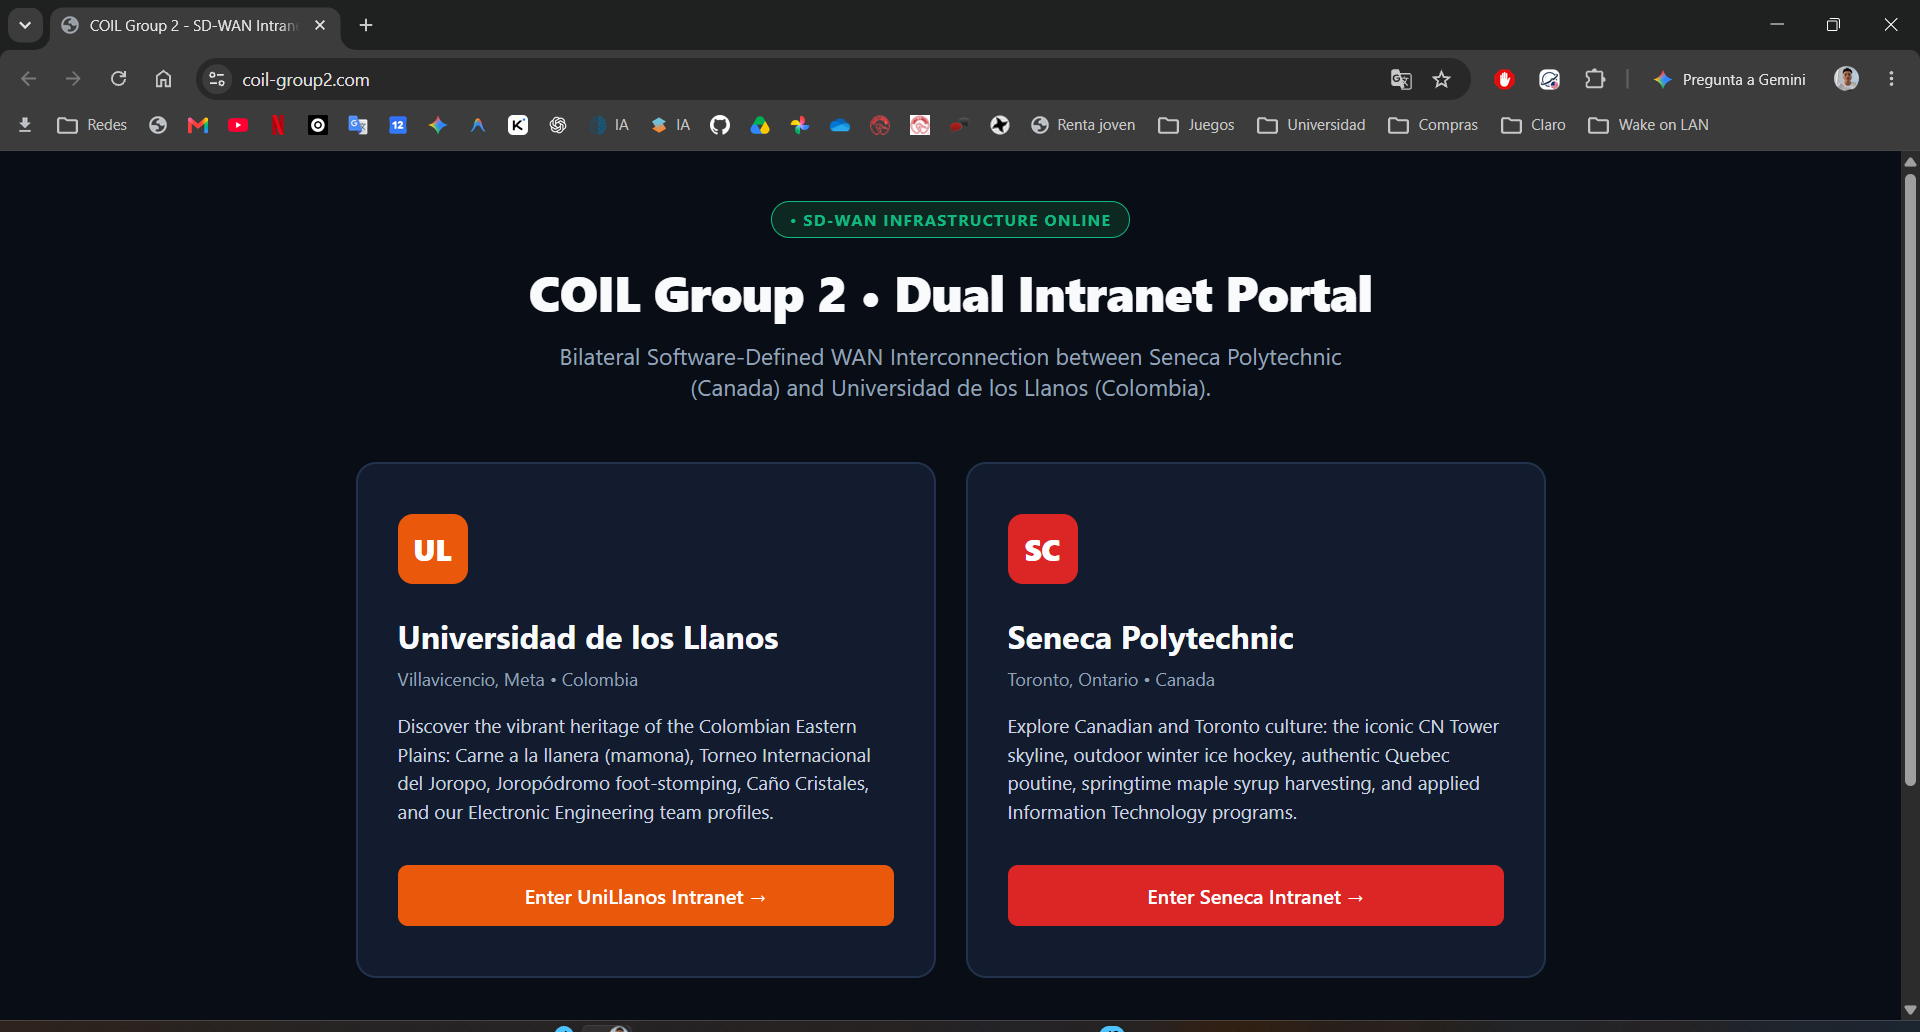
\includegraphics[width=0.90\textwidth]{figuras/ui_portal_fresh.png}
\caption{COIL Group~2 Dual Intranet Gateway Portal (\texttt{portal/index.html}, \qty{6941}{\byte}) rendered at \texttt{https://www.coil-group2.com/}, featuring the \textit{SD-WAN Infrastructure Online} badge, institutional \texttt{UL} and \texttt{SC} routing cards, and the bottom SD-WAN telemetry bar.}
\label{fig:ui_portal}
\end{figure*}

\textbf{1) Dual Intranet Gateway Portal (Fig.~\ref{fig:ui_portal}, Appendix~\ref{app:portal_html}):} Served at \nolinkurl{/} (\qty{6941}{\byte}), the gateway opens with an emerald status pill (\textit{SD-WAN Infrastructure Online}, \texttt{\#10b981}) above the bilateral title header. Its central CSS Grid (\texttt{repeat(auto-fit, minmax(300px, 1fr))}) presents two interactive institutional routing cards: \texttt{UL} (\textit{Universidad de los Llanos}, Villavicencio, Meta, styled with \texttt{\#ea580c} orange accents) and \texttt{SC} (\textit{Seneca Polytechnic}, Toronto, Ontario, styled with \texttt{\#dc2626} crimson accents), each applying a \texttt{translateY(-6px)} hover elevation and colored box-shadow transition. Below the cards, the telemetry status bar (\texttt{.network-bar}) displays four live infrastructure indicators: \textit{SD-WAN Mesh: ZeroTier Virtual Ethernet}, \textit{Host IP: 172.22.201.2}, \textit{Encryption: TLS 1.3 / HTTPS (Port 443)}, and \textit{Domain: www.coil-group2.com}. On narrow viewports, the \texttt{@media (max-width: 640px)} rule collapses \texttt{.gateways} to a single column (\texttt{1fr}) and stacks \texttt{.network-bar} items vertically.

\begin{figure*}[t]
\centering
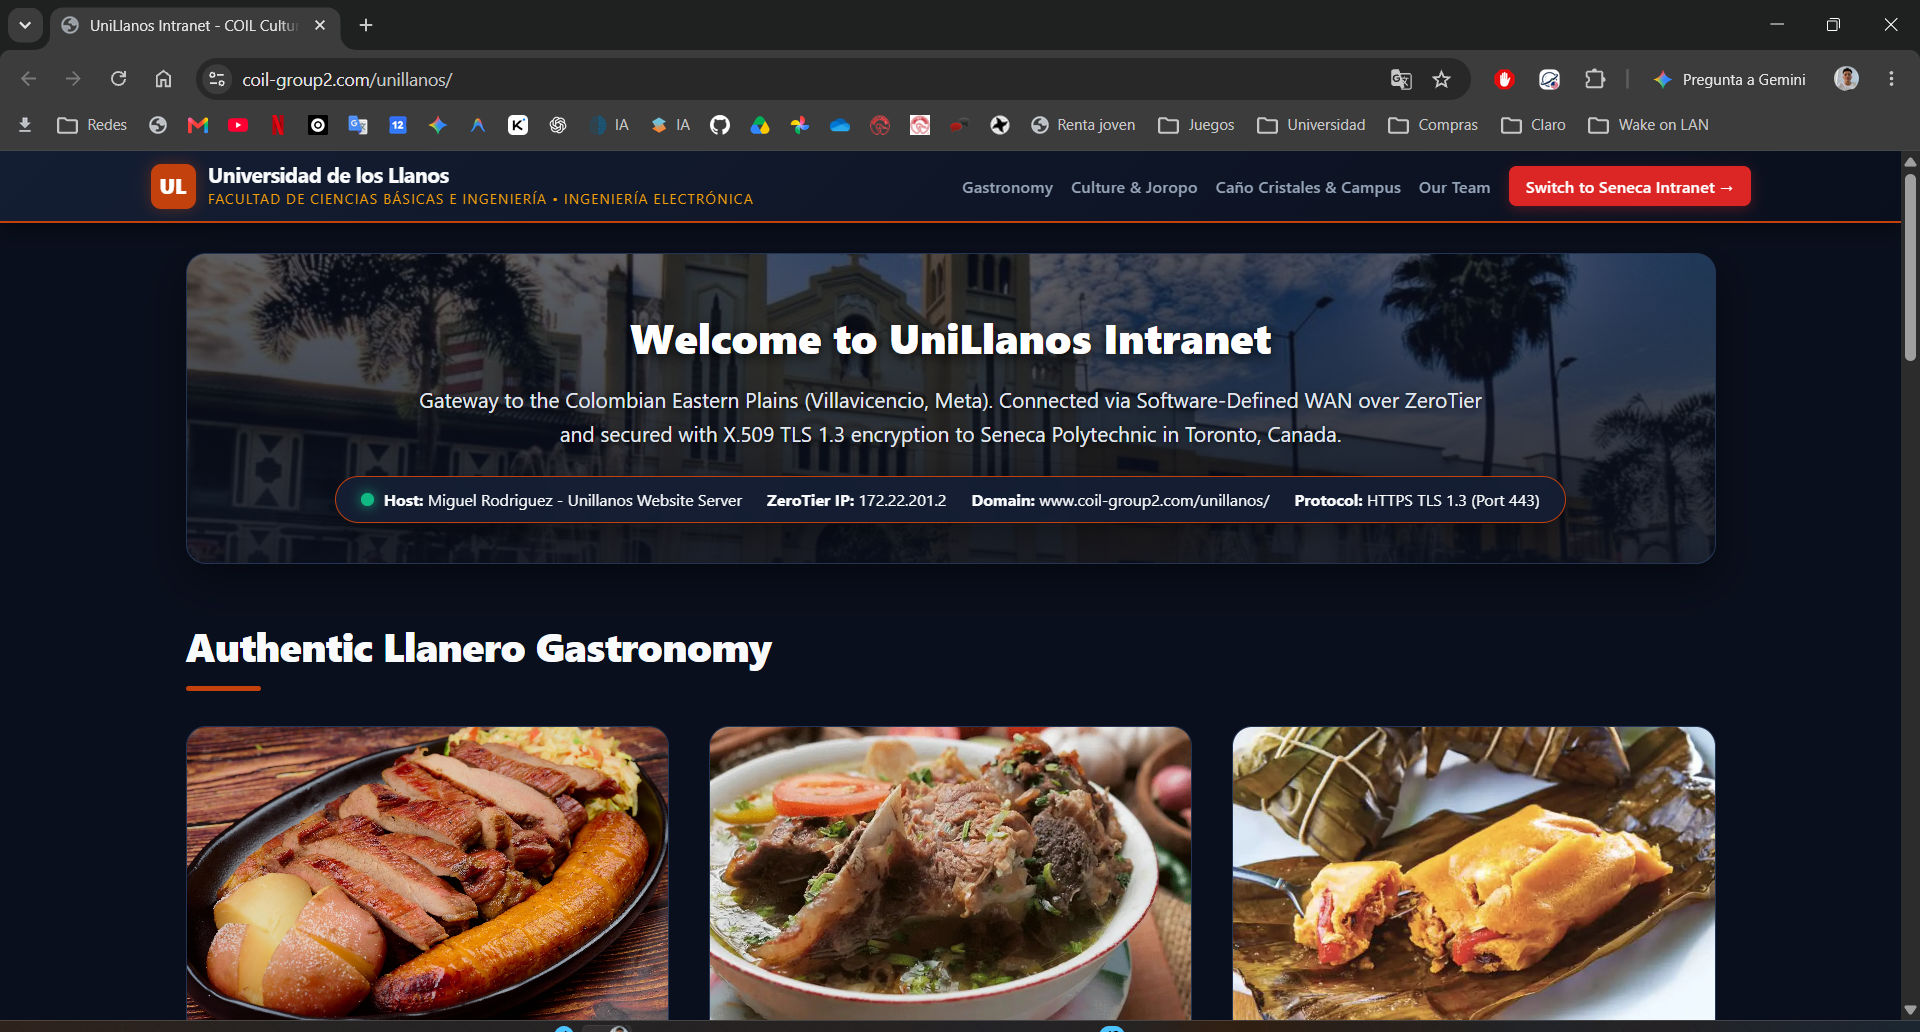
\includegraphics[width=0.90\textwidth]{figuras/ui_unillanos_fresh.png}
\caption{Universidad de los Llanos Cultural Intranet (\texttt{unillanos/index.html}, \qty{18520}{\byte}) rendered at \texttt{https://www.coil-group2.com/unillanos/}, showing the sticky \texttt{UL} navigation bar with the red \textit{Switch to Seneca Intranet} control, Villavicencio panorama hero with glassmorphism telemetry pill, Llanero cultural cards, and Engineering Team profiles.}
\label{fig:ui_unillanos}
\end{figure*}

\textbf{2) Universidad de los Llanos Intranet (Fig.~\ref{fig:ui_unillanos}, Appendix~\ref{app:unillanos_html}):} Served at \nolinkurl{/unillanos/} (\qty{18520}{\byte}), the Colombian portal features a sticky top navbar displaying the \texttt{UL} badge, faculty subtitle (\textit{Facultad de Ciencias B\'{a}sicas e Ingenier\'{i}a $\cdot$ Ingenier\'{i}a Electr\'{o}nica}), smooth anchor links (\texttt{\#gastronomy}, \texttt{\#festivals}, \texttt{\#nature}, \texttt{\#team}), and a prominent red (\texttt{\#dc2626}) \textit{Switch to Seneca Intranet} cross-routing button targeting \nolinkurl{/seneca/}. Its hero banner overlays \nolinkurl{img/villavicencio_panorama.jpg} with a glassmorphism telemetry pill (\texttt{backdrop-filter: blur(8px)}) embedding a glowing green status dot, \textit{Host: Miguel Rodriguez - Unillanos Website Server}, \textit{ZeroTier IP: 172.22.201.2}, \textit{Domain: www.coil-group2.com/unillanos/}, and \textit{Protocol: HTTPS TLS 1.3 (Port 443)}. Eight photographic cards with hover zoom (\texttt{scale(1.06)}) showcase Llanero gastronomy (\textit{Carne a la Llanera (Mamona)}, \textit{Caldo de Costilla}, \textit{Hayaca Llanera}), regional festivals and landscapes (\textit{Torneo del Joropo \& Jorop\'{o}dromo}, \textit{Sunsets of the Orinoco Basin}, \textit{Villavicencio Metropolis}), and natural heritage (\textit{Ca\~{n}o Cristales: River of Five Colors}, \textit{UniLlanos Barcelona Campus}). Below the grids, the \textit{UniLlanos Engineering Team} showcase presents circular avatar biographies for \textit{Miguel \'{A}ngel Rodr\'{i}guez Payares} (10th Semester, Electronic Engineering, lead server architect) and \textit{Luis Alejandro Le\'{o}n Vel\'{a}squez} (9th Semester, Electronic Engineering, English~C1). Under \texttt{@media (max-width: 768px)}, the navbar converts \texttt{.nav-links} into a touch-scrollable horizontal bar (\texttt{-webkit-overflow-scrolling: touch}), expands the partner button to full width, and centers team profiles vertically.

\begin{figure*}[t]
\centering
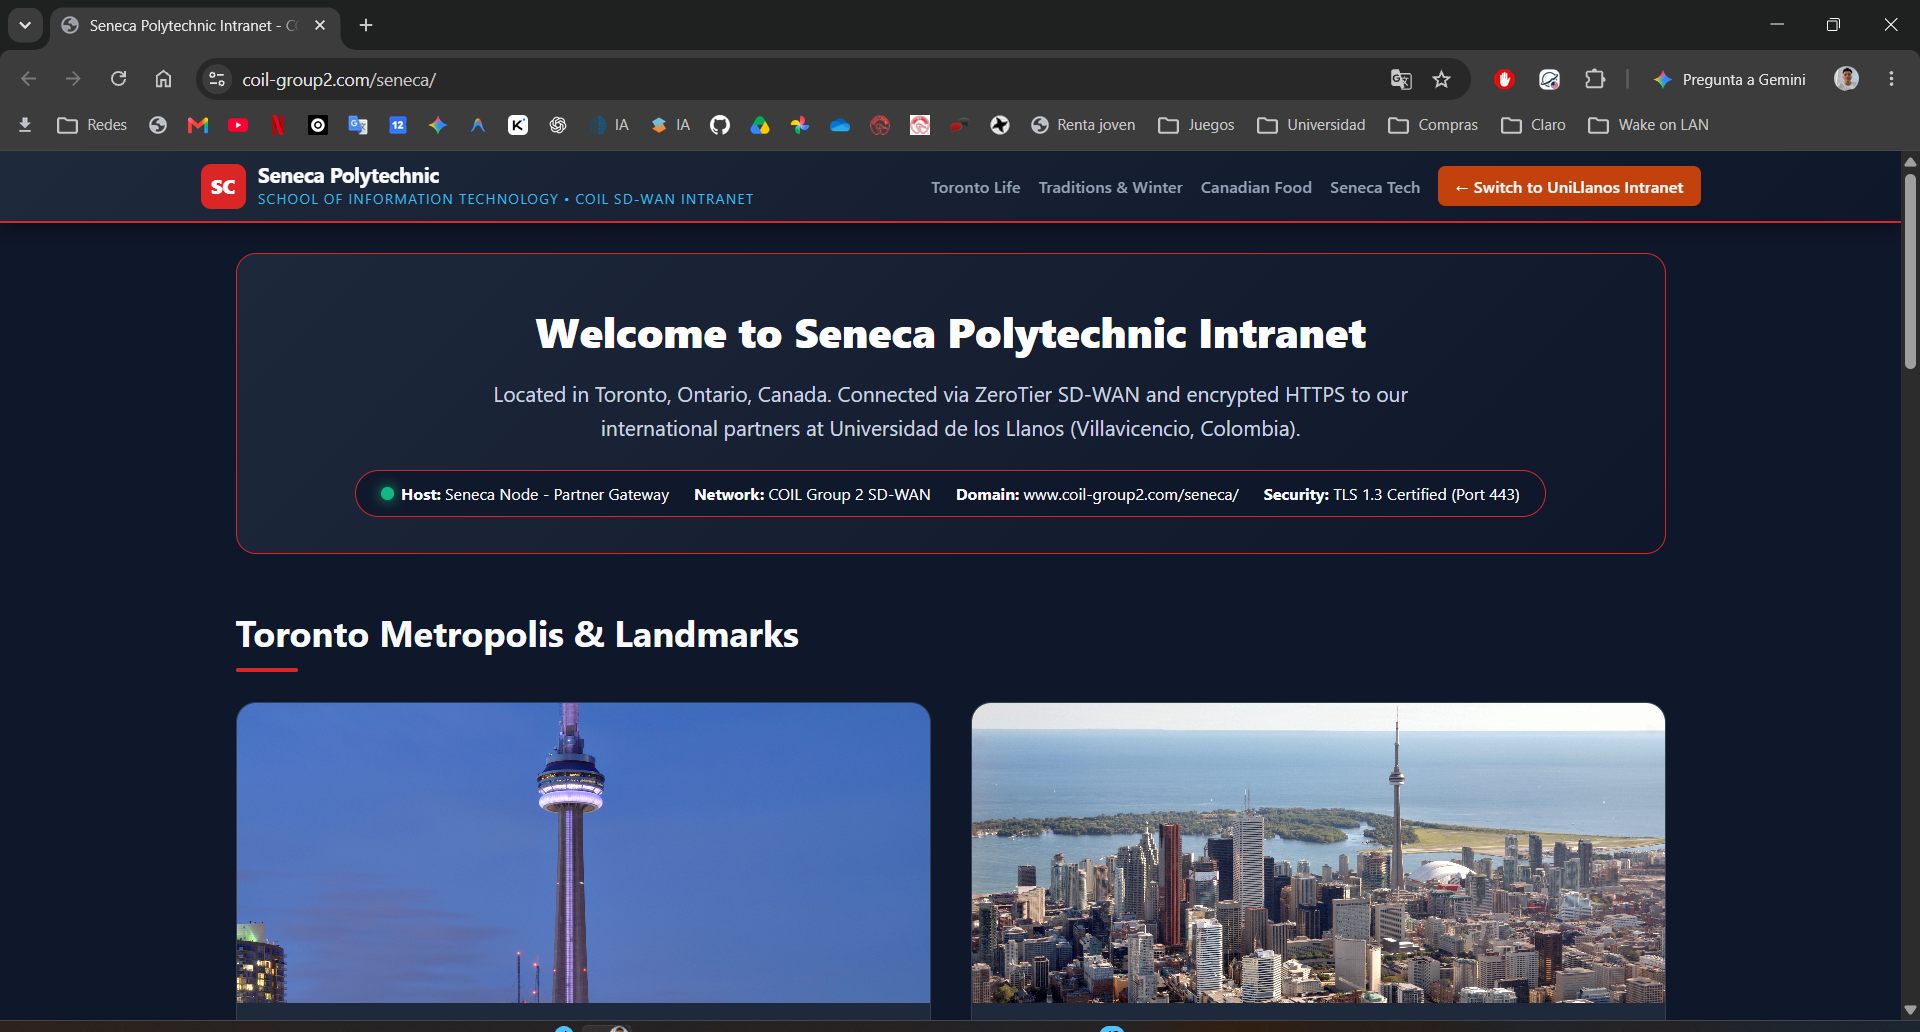
\includegraphics[width=0.90\textwidth]{figuras/ui_seneca_fresh.png}
\caption{Seneca Polytechnic Cultural Intranet (\texttt{seneca/index.html}, \qty{15470}{\byte}) rendered at \texttt{https://www.coil-group2.com/seneca/}, displaying the sticky \texttt{SC} header with the orange \textit{Switch to UniLlanos Intranet} return control, gateway telemetry pill, and Canadian cultural, culinary, and IT showcase cards.}
\label{fig:ui_seneca}
\end{figure*}

\textbf{3) Seneca Polytechnic Intranet (Fig.~\ref{fig:ui_seneca}, Appendix~\ref{app:seneca_html}):} Served at \nolinkurl{/seneca/} (\qty{15470}{\byte}), the Canadian partner portal mirrors the UniLlanos design system with crimson (\texttt{\#dc2626}) and sky-blue (\texttt{\#38bdf8}) accents. Its sticky header presents the \texttt{SC} badge, \textit{School of Information Technology $\cdot$ COIL SD-WAN Intranet} subheading, section anchors (\texttt{\#toronto}, \texttt{\#canadian-culture}, \texttt{\#gastronomy}, \texttt{\#academics}), and the reciprocal burnt-orange (\texttt{\#c2410c}) \textit{Switch to UniLlanos Intranet} button returning to \nolinkurl{/unillanos/}. The hero houses the partner telemetry pill (\textit{Host: Seneca Node - Partner Gateway}, \textit{Network: COIL Group 2 SD-WAN}, \textit{Domain: www.coil-group2.com/seneca/}, \textit{Security: TLS 1.3 Certified (Port 443)}), followed by eight lazy-loaded (\texttt{loading="lazy"}) cards across four domains: Toronto landmarks (\textit{CN Tower \& Downtown Skyline} at \qty{553.3}{\meter}, \textit{Lake Ontario \& Toronto Islands}), Canadian traditions (\textit{Ice Hockey \& Outdoor Rinks}, \textit{Maple Syrup \& Sugar Shacks}), culinary classics (\textit{Authentic Poutine}, \textit{Peameal Bacon \& Butter Tarts}), and bilateral academics (\textit{School of Information Technology}, \textit{UniLlanos $\cdot$ Seneca COIL Exchange}), sharing the identical \texttt{@media (max-width: 768px)} mobile touch layout.

\subsection{Manual 3 (15\%): Self-Signed SSL/TLS PKI and Browser Trust Remediation (Bonus)}
\label{subsec:manual3_pki}

Modern browsers enforce RFC~5280 X.509v3 certificate chain validation~\cite{rfc5280} and reject simple self-signed leaf certificates that lack Subject Alternative Name (SAN) extensions or a trusted Root Certificate Authority (CA) anchor. To satisfy the mandatory HTTPS encryption requirement over TLS~1.3~\cite{rfc8446} while earning the bonus credit for eliminating browser security warnings (\texttt{NET::ERR\_CERT\_AUTHORITY\_INVALID}), a two-tier private Public Key Infrastructure (PKI) was engineered using OpenSSL~\cite{openssl2024}, as depicted in Figure~\ref{fig:pki_architecture}.

\begin{figure*}[htbp]
\centering
\definecolor{pkiGoldFill}{HTML}{FEF3C7}
\definecolor{pkiGoldLine}{HTML}{B45309}
\definecolor{pkiGoldBg}{HTML}{FFFBEB}
\definecolor{pkiBlueFill}{HTML}{DBEAFE}
\definecolor{pkiBlueLine}{HTML}{1D4ED8}
\definecolor{pkiBlueBg}{HTML}{EFF6FF}
\definecolor{pkiIndigoFill}{HTML}{E0E7FF}
\definecolor{pkiIndigoLine}{HTML}{3730A3}
\definecolor{pkiPurpleFill}{HTML}{EDE9FE}
\definecolor{pkiPurpleLine}{HTML}{6D28D9}
\definecolor{pkiPurpleBg}{HTML}{F5F3FF}
\definecolor{pkiGreenFill}{HTML}{D1FAE5}
\definecolor{pkiGreenLine}{HTML}{047857}
\definecolor{pkiGreenBg}{HTML}{ECFDF5}
\definecolor{pkiRedFill}{HTML}{FEE2E2}
\definecolor{pkiRedLine}{HTML}{B91C1C}
\definecolor{pkiSlateFill}{HTML}{F1F5F9}
\definecolor{pkiSlateLine}{HTML}{475569}

\resizebox{0.96\textwidth}{!}{%
\begin{tikzpicture}[
    >=Stealth,
    every node/.style={font=\scriptsize, text=black!88},
    node distance=0.45cm and 0.55cm,
    card/.style={
        rectangle, rounded corners=3pt, draw=pkiSlateLine, fill=white,
        line width=0.75pt, inner sep=5.5pt, align=left
    },
    card_gold/.style={card, draw=pkiGoldLine, fill=white},
    card_blue/.style={card, draw=pkiBlueLine, fill=white},
    card_indigo/.style={card, draw=pkiIndigoLine, fill=pkiIndigoFill!35},
    card_purple/.style={card, draw=pkiPurpleLine, fill=white},
    card_green/.style={card, draw=pkiGreenLine, fill=white},
    card_err/.style={card, draw=pkiRedLine, fill=pkiRedFill!75, align=center},
    card_ok/.style={card, draw=pkiGreenLine, fill=pkiGreenFill!85, align=center},
    hdr_pill/.style={
        rectangle, rounded corners=2pt, font=\scriptsize\bfseries,
        inner xsep=6pt, inner ysep=2.5pt, text=white
    },
    zone_box/.style={
        rectangle, rounded corners=6pt, dashed, line width=0.85pt, inner sep=8pt
    },
    flow_arr/.style={
        -{Stealth[length=5pt, width=3.5pt]},
        line width=0.95pt, color=pkiSlateLine, shorten >=1.5pt, shorten <=1pt
    },
    flow_short/.style={
        -{Stealth[length=4pt, width=2.8pt]},
        line width=0.85pt, color=pkiSlateLine, shorten >=1pt, shorten <=0.5pt
    },
    rail_gold/.style={
        -{Stealth[length=5pt, width=3.5pt]},
        line width=0.95pt, color=pkiGoldLine, rounded corners=4pt, shorten >=1.5pt
    },
    verify_arr/.style={
        {Stealth[length=4.5pt, width=3pt]}-{Stealth[length=4.5pt, width=3pt]},
        line width=0.95pt, densely dashed, color=pkiGreenLine, shorten >=1.5pt, shorten <=1.5pt
    },
    edge_tag/.style={
        font=\tiny\bfseries, fill=white, inner xsep=3.5pt, inner ysep=1.5pt,
        rounded corners=1.5pt, draw=black!20, line width=0.35pt, align=center
    },
]

\node[card_gold, text width=6.6cm, minimum height=2.15cm] (ca_id) at (0,0) {%
    \textbf{\footnotesize COIL Group 2 Root CA}\\[2pt]
    {\tiny\color{pkiGoldLine}\textbf{Self-Signed Root Authority (Offline)}}\\[3pt]
    $\bullet$ \textbf{Subject/Issuer:} \texttt{CN = COIL Group 2 Root CA}\\
    $\bullet$ \textbf{Cert:} \texttt{COIL\_Group2\_Root\_CA.crt} / \texttt{ca-cert.pem}\\
    $\bullet$ \textbf{Signing Key:} \texttt{ca-key.pem} (offline private key)
};

\node[card_gold, text width=7.1cm, minimum height=2.15cm, right=0.55cm of ca_id] (ca_specs) {%
    \textbf{Cryptographic Profile \& X.509v3 Constraints}\\[3pt]
    $\bullet$ \textbf{Key / Hash:} \texttt{2048-bit RSA}, SHA-256 self-signed\\
    $\bullet$ \textbf{Extensions:} \texttt{CA:TRUE}, \texttt{keyCertSign}, \texttt{cRLSign}\\
    $\bullet$ \textbf{Serial:} \texttt{1CB6...57D0}\\
    $\bullet$ \textbf{Validity:} Nov 21, 2026 -- Nov 18, 2036 (\qty{3650}{days})
};

\coordinate (t1_mid_top) at ($(ca_id.north west)!0.5!(ca_specs.north east)$);
\coordinate (t1_mid_bot) at ($(ca_id.south west)!0.5!(ca_specs.south east)$);

\node[hdr_pill, fill=pkiGoldLine, anchor=south west] (t1_hdr)
    at ($(ca_id.north west)+(0,0.18cm)$)
    {TIER 1: Offline Root Authority};

\begin{pgfonlayer}{background}
    \node[zone_box, draw=pkiGoldLine, fill=pkiGoldBg, fit=(t1_hdr)(ca_id)(ca_specs)] (zone_t1) {};
\end{pgfonlayer}

\node[rectangle, rounded corners=3pt, fill=pkiSlateFill, draw=pkiSlateLine!45,
      line width=0.6pt, inner xsep=12pt, inner ysep=4pt,
      font=\small\bfseries, text=black!90, anchor=south] (fig_title)
    at ($(zone_t1.north -| t1_mid_top)+(0,0.42cm)$)
    {COIL Group 2 -- Custom Root CA PKI, X.509v3 SANs, TLS 1.3 Stack \& Trust Remediation};

\coordinate (t2_row_top) at ($(zone_t1.south -| t1_mid_bot)+(0,-1.65cm)$);

\node[card_blue, text width=4.45cm, minimum height=3.20cm, anchor=north] (leaf_crt)
    at (t2_row_top) {%
    \textbf{Leaf Certificate (\texttt{server.crt})}\\[2pt]
    \textbf{Subject:} \texttt{CN = www.coil-group2.com}\\[3pt]
    $\bullet$ \textbf{Constraints:} \texttt{CA:FALSE}\\
    $\bullet$ \textbf{Key Usage:} \texttt{digitalSignature},\\
    \hspace*{1.2em}\texttt{keyEncipherment}\\
    $\bullet$ \textbf{EKU:} \texttt{serverAuth}, \texttt{clientAuth}\\
    $\bullet$ \textbf{Serial:} \texttt{173D...87D7}\\
    $\bullet$ \textbf{Valid:} Nov 21, 2026 -- Feb 23, 2029\\
    \hspace*{1.2em}(\qty{825}{days})
};

\node[card_blue, text width=3.05cm, minimum height=1.42cm, anchor=north east] (t2_cnf)
    at ($(leaf_crt.north west)+(-0.65cm,0)$) {%
    \textbf{OpenSSL Policy}\\[2pt]
    \texttt{openssl.cnf}\\
    {\tiny Profiles: \texttt{[v3\_ca]} \& \texttt{[server\_ext]}}
};

\node[card_blue, text width=3.05cm, minimum height=1.42cm, anchor=south east] (t2_csr)
    at (leaf_crt.south west -| t2_cnf.east) {%
    \textbf{Signing Request}\\[2pt]
    \texttt{server.csr}\\
    {\tiny Signed by \texttt{ca-key.pem}}
};

\node[card_indigo, text width=4.05cm, minimum height=3.20cm, anchor=north west] (san_box)
    at ($(leaf_crt.north east)+(0.95cm,0)$) {%
    \textbf{X.509v3 SAN Extension}\\[1pt]
    {\tiny\color{pkiIndigoLine}\textbf{Subject Alternative Name (\texttt{[alt\_names]})}}\\[3pt]
    \textbf{DNS Entries (5):}\\
    {\tiny\texttt{www.coil-group2.com}\\[0.5pt]
    \texttt{coil-group2.com}\\[0.5pt]
    \texttt{unillanos.coil-group2.com}\\[0.5pt]
    \texttt{seneca.coil-group2.com}\\[0.5pt]
    \texttt{localhost}}\\[3pt]
    \textbf{IP Entries (4):}\\
    {\tiny\texttt{172.22.201.2}, \texttt{172.22.31.69},\\[0.5pt]
    \texttt{10.51.76.174}, \texttt{127.0.0.1}}
};

\node[hdr_pill, fill=pkiBlueLine, anchor=south west] (t2_hdr)
    at ($(t2_cnf.north west)+(0,0.18cm)$)
    {TIER 2: OpenSSL \& Leaf CA};

\begin{pgfonlayer}{background}
    \node[zone_box, draw=pkiBlueLine, fill=pkiBlueBg, fit=(t2_hdr)(t2_cnf)(t2_csr)(leaf_crt)(san_box)] (zone_t2) {};
\end{pgfonlayer}

\def\coloffset{4.90cm}
\coordinate (t3_top_y) at ($(zone_t2.south -| t1_mid_bot)+(0,-1.75cm)$);
\coordinate (t3A_center_top) at ($(t3_top_y)+(-\coloffset,0)$);
\coordinate (t3B_center_top) at ($(t3_top_y)+(+\coloffset,0)$);

\node[card_purple, text width=6.95cm, minimum height=1.05cm, anchor=north] (pA_bundle) at (t3A_center_top) {%
    \textbf{TLS Certificate Chain \& Private Key Bundle}\\[2pt]
    \texttt{fullchain.pem} (\texttt{server.crt} + \texttt{ca-cert.pem}) + \texttt{server-key.pem}
};

\node[card_purple, text width=6.95cm, minimum height=1.28cm, below=0.45cm of pA_bundle] (pA_ctx) {%
    \textbf{Python HTTPS Server Context}\\[2pt]
    \texttt{ssl.SSLContext(PROTOCOL\_TLS\_SERVER)}\\
    ALPN: \texttt{http/1.1} \quad$\cdot$\quad Cipher: \texttt{TLS\_AES\_256\_GCM\_SHA384}
};

\coordinate (row3_top_y) at ($(pA_ctx.south)+(0,-0.55cm)$);

\node[card_purple, text width=3.20cm, minimum height=1.18cm, align=center, anchor=north west] (pA_uni)
    at (pA_ctx.west |- row3_top_y) {%
    \textbf{UniLlanos Server}\\
    \texttt{172.22.201.2:443}
};

\node[card_purple, text width=3.20cm, minimum height=1.18cm, align=center, anchor=north east] (pA_sen)
    at (pA_ctx.east |- row3_top_y) {%
    \textbf{Seneca Gateway}\\
    \texttt{172.22.31.69:443}
};

\node[hdr_pill, fill=pkiPurpleLine, anchor=south west] (pA_hdr)
    at ($(pA_bundle.north west)+(0,0.18cm)$)
    {TIER 3A: Server TLS 1.3 Stack};

\begin{pgfonlayer}{background}
    \node[zone_box, draw=pkiPurpleLine, fill=pkiPurpleBg, fit=(pA_hdr)(pA_bundle)(pA_ctx)(pA_uni)(pA_sen)] (zone_3A) {};
\end{pgfonlayer}

\node[card_green, text width=6.95cm, minimum height=1.05cm, anchor=north] (pB_dist) at (t3B_center_top) {%
    \textbf{Root CA Distribution Mechanism}\\[2pt]
    \texttt{COIL\_Group2\_Root\_CA.crt} (served via \texttt{/ca.crt} or \texttt{install\_root\_ca.ps1})
};

\node[card_green, text width=3.85cm, minimum height=1.28cm, anchor=north west] (pB_win)
    at ($(pB_dist.south west)+(0,-0.45cm)$) {%
    \textbf{Windows Trust Store}\\
    \texttt{Cert:\textbackslash LocalMachine\textbackslash Root}\\
    {\tiny Thumbprint: \texttt{6C94...E0D9}}
};

\node[card_green, text width=2.55cm, minimum height=1.28cm, anchor=north east] (pB_and)
    at ($(pB_dist.south east)+(0,-0.45cm)$) {%
    \textbf{Android OS}\\
    Android Trusted\\
    Credentials
};

\node[card_err, text width=3.22cm, minimum height=1.18cm, anchor=north west] (pB_err)
    at (pB_dist.west |- row3_top_y) {%
    \textbf{Eliminates Warning}\\[2pt]
    {\fontsize{4.6}{6}\selectfont\texttt{NET::ERR\_CERT\_AUTHORITY\_INVALID}}
};

\node[card_ok, text width=2.45cm, minimum height=1.18cm, anchor=north east] (pB_ok)
    at (pB_dist.east |- row3_top_y) {%
    \textbf{Verified Trusted}\\
    \textbf{HTTPS Padlock}\\
    {\tiny Chrome \& Mobile}
};

\node[hdr_pill, fill=pkiGreenLine, anchor=south west] (pB_hdr)
    at ($(pB_dist.north west)+(0,0.18cm)$)
    {TIER 3B: Client Trust Store (Bonus)};

\begin{pgfonlayer}{background}
    \node[zone_box, draw=pkiGreenLine, fill=pkiGreenBg, fit=(pB_hdr)(pB_dist)(pB_win)(pB_and)(pB_err)(pB_ok)] (zone_3B) {};
\end{pgfonlayer}

\coordinate (t1_sign_exit) at (zone_t1.south -| leaf_crt.north);
\draw[flow_arr] (t1_sign_exit) -- (leaf_crt.north);
\node[edge_tag] at ($(t1_sign_exit)!0.50!(t1_sign_exit |- zone_t2.north)$)
    {Signs CSR w/ \texttt{ca-key.pem}};

\coordinate (t2_join) at ($(leaf_crt.west)+(-0.32cm,0)$);
\draw[line width=0.85pt, color=pkiSlateLine] (t2_cnf.east) -| (t2_join);
\draw[line width=0.85pt, color=pkiSlateLine] (t2_csr.east) -| (t2_join);
\draw[flow_short] (t2_join) -- (leaf_crt.west);

\draw[flow_short] (leaf_crt.east) -- node[edge_tag, above=4pt] {Embeds} (leaf_crt.east -| san_box.west);

\coordinate (pA_crt_in) at ($(pA_bundle.north east)+(-0.95cm,0)$);
\coordinate (bus_t2_t3) at ($(zone_t2.south)!0.50!(zone_3A.north)$);
\draw[flow_arr, rounded corners=4pt]
    (leaf_crt.south) -- (leaf_crt.south |- bus_t2_t3)
    -| (pA_crt_in);
\node[edge_tag] at ($(leaf_crt.south |- bus_t2_t3)!0.48!(pA_crt_in |- bus_t2_t3)$)
    {\texttt{server.crt} (Leaf)};

\coordinate (rail_L_x) at ($(zone_3A.west)+(-0.62cm,0)$);
\draw[rail_gold]
    (zone_t1.west) -- (zone_t1.west -| rail_L_x)
    |- (pA_bundle.west);
\node[edge_tag, text=pkiGoldLine, draw=pkiGoldLine!60, anchor=center]
    at (rail_L_x |- leaf_crt.center)
    {\texttt{ca-cert.pem}\\[1pt](Chain Anchor)};

\coordinate (rail_R_x) at ($(zone_3B.east)+(0.62cm,0)$);
\draw[rail_gold]
    (zone_t1.east) -- (zone_t1.east -| rail_R_x)
    |- (pB_dist.east);
\node[edge_tag, text=pkiGoldLine, draw=pkiGoldLine!60, anchor=center]
    at (rail_R_x |- san_box.center)
    {\texttt{COIL\_Group2\_}\\[1pt]\texttt{Root\_CA.crt}\\[1pt](Trust Anchor)};

\draw[flow_short] (pA_bundle.south) -- (pA_ctx.north);
\coordinate (pA_split) at ($(pA_ctx.south)!0.45!(pA_uni.north -| pA_ctx.south)$);
\draw[line width=0.85pt, color=pkiSlateLine] (pA_ctx.south) -- (pA_split);
\draw[flow_short, rounded corners=3pt] (pA_split) -| (pA_uni.north);
\draw[flow_short, rounded corners=3pt] (pA_split) -| (pA_sen.north);

\coordinate (pB_split) at ($(pB_dist.south)!0.45!(pB_win.north -| pB_dist.south)$);
\draw[line width=0.85pt, color=pkiSlateLine] (pB_dist.south) -- (pB_split);
\draw[flow_short, rounded corners=3pt] (pB_split) -| (pB_win.north);
\draw[flow_short, rounded corners=3pt] (pB_split) -| (pB_and.north);

\draw[flow_short] (pB_win.south) -- (pB_win.south |- pB_err.north);
\draw[flow_short] (pB_and.south) -- (pB_and.south |- pB_ok.north);
\draw[flow_short, color=pkiGreenLine] (pB_err.east) -- (pB_ok.west);

\draw[verify_arr] (pA_sen.east) -- (pB_err.west);
\node[edge_tag, text=pkiGreenLine, draw=pkiGreenLine!60, anchor=south]
    at ($(pA_sen.east)!0.5!(pB_err.west)+(0,0.14cm)$)
    {TLS 1.3 +\\[1pt]SAN Match};

\coordinate (bot_mid) at ($(zone_3A.south west)!0.5!(zone_3B.south east)+(0,-0.45cm)$);

\node[font=\scriptsize\bfseries, anchor=north] (leg_hdr) at (bot_mid)
    {Architecture Legend \& Cryptographic Flow Semantics};

\node[font=\tiny, anchor=north, align=center] (leg_r1) at ($(leg_hdr.south)+(0,-0.12cm)$) {%
    \fcolorbox{pkiGoldLine}{pkiGoldBg}{\rule{0pt}{4.2pt}\rule{6.5pt}{0pt}}\, Tier 1: Offline Root CA \qquad
    \fcolorbox{pkiBlueLine}{pkiBlueBg}{\rule{0pt}{4.2pt}\rule{6.5pt}{0pt}}\, Tier 2: OpenSSL Policy \& SAN Leaf \qquad
    \fcolorbox{pkiPurpleLine}{pkiPurpleBg}{\rule{0pt}{4.2pt}\rule{6.5pt}{0pt}}\, Tier 3A: Server TLS 1.3 Stack \qquad
    \fcolorbox{pkiGreenLine}{pkiGreenBg}{\rule{0pt}{4.2pt}\rule{6.5pt}{0pt}}\, Tier 3B: Client Trust Store (Bonus)
};

\coordinate (leg_r2_y) at ($(leg_r1.south)+(0,-0.32cm)$);

\node[font=\tiny, anchor=west] (ar2_txt) at ($(leg_r2_y)+(-0.95cm,0)$) {Root CA Distribution Rail};
\draw[rail_gold] ($(ar2_txt.west)+(-0.72cm,0)$) -- ($(ar2_txt.west)+(-0.06cm,0)$);
\coordinate (ar2_start) at ($(ar2_txt.west)+(-0.75cm,0)$);

\node[font=\tiny, anchor=east] (ar1_txt) at ($(ar2_start)+(-0.90cm,0)$) {Signing / Deployment Flow};
\draw[flow_short] ($(ar1_txt.west)+(-0.72cm,0)$) -- ($(ar1_txt.west)+(-0.06cm,0)$);
\coordinate (ar1_start) at ($(ar1_txt.west)+(-0.75cm,0)$);

\node[font=\tiny, anchor=west] (ar3_txt) at ($(ar2_txt.east)+(1.62cm,0)$) {Verified TLS 1.3 Chain \& SAN Handshake};
\draw[verify_arr] ($(ar3_txt.west)+(-0.72cm,0)$) -- ($(ar3_txt.west)+(-0.06cm,0)$);

\coordinate (leg_flush_L) at (zone_3A.west |- leg_hdr.north);
\coordinate (leg_flush_R) at (zone_3B.east |- ar3_txt.south);

\begin{pgfonlayer}{background}
    \node[rectangle, rounded corners=4pt, draw=pkiSlateLine!45, fill=pkiSlateFill,
          line width=0.6pt, inner xsep=0pt, inner ysep=5pt,
          fit=(leg_flush_L)(leg_flush_R)(leg_hdr)(leg_r1)(ar1_start)(ar3_txt)] (legend_bar) {};
\end{pgfonlayer}

\end{tikzpicture}%
}
\caption{Three-tier Public Key Infrastructure (PKI) and browser trust remediation architecture. Tier~1 establishes the offline 2048-bit RSA \texttt{COIL Group 2 Root CA} (\qty{3650}{days}); Tier~2 signs the leaf certificate (\texttt{server.crt}, \qty{825}{days}) with five DNS and four IPv4 Subject Alternative Names (SANs); Tier~3A deploys \texttt{fullchain.pem} to the dual-node TLS~1.3 server stack while Tier~3B imports \texttt{COIL\_Group2\_Root\_CA.crt} into Windows and Android root trust stores to eliminate \texttt{NET::ERR\_CERT\_AUTHORITY\_INVALID} warnings (bonus criterion).}
\label{fig:pki_architecture}
\end{figure*}


\subsubsection{Step 1: OpenSSL X.509v3 Configuration Policy (\texttt{openssl.cnf})}
Create the OpenSSL configuration file \texttt{modulo2/certificados/openssl.cnf} defining two distinct X.509v3 extension profiles: \texttt{[v3\_ca]} for the offline Root CA (\texttt{basicConstraints = critical, CA:true}, \texttt{keyUsage = critical, digitalSignature, cRLSign, keyCertSign}) and \texttt{[server\_ext]} for the multi-tenant server leaf certificate (\texttt{basicConstraints = CA:FALSE}, \texttt{extendedKeyUsage = serverAuth, clientAuth}, and \texttt{subjectAltName = @alt\_names}). The SAN block binds all five DNS hostnames and four IPv4 addresses used across the SD-WAN overlay:

\begin{lstlisting}[caption={X.509v3 Subject Alternative Name declaration in \texttt{openssl.cnf}.},label={lst:manual3_san}]
[ server_ext ]
subjectKeyIdentifier   = hash
authorityKeyIdentifier = keyid,issuer
basicConstraints       = CA:FALSE
keyUsage               = digitalSignature, keyEncipherment
extendedKeyUsage       = serverAuth, clientAuth
subjectAltName         = @alt_names

[ alt_names ]
DNS.1 = www.coil-group2.com
DNS.2 = coil-group2.com
DNS.3 = unillanos.coil-group2.com
DNS.4 = seneca.coil-group2.com
DNS.5 = localhost
IP.1  = 172.22.201.2
IP.2  = 172.22.31.69
IP.3  = 10.51.76.174
IP.4  = 127.0.0.1
\end{lstlisting}

\subsubsection{Step 2: Root CA Generation (\qty{3650}{days})}
Generate the 2048-bit RSA private key (\texttt{ca-key.pem}) and self-sign the offline Root CA certificate (\texttt{ca-cert.pem} and \texttt{COIL\_Group2\_Root\_CA.crt}) using SHA-256 for a ten-year validity period:

\begin{lstlisting}[caption={Generating the private 2048-bit RSA Root Certificate Authority.},label={lst:manual3_rootca}]
openssl genrsa -out ca-key.pem 2048
openssl req -x509 -new -nodes -key ca-key.pem -sha256 -days 3650 \
  -out ca-cert.pem -config openssl.cnf -extensions v3_ca
Copy-Item ca-cert.pem COIL_Group2_Root_CA.crt
\end{lstlisting}

\subsubsection{Step 3: Server Leaf Certificate Signing and Chain Bundling (\qty{825}{days})}
Generate the server private key (\texttt{server-key.pem}), create the Certificate Signing Request (\texttt{server.csr}) using the \texttt{[server\_req]} profile, sign the leaf certificate (\texttt{server.crt}) for \qty{825}{days} (adhering to the Apple/Chromium maximum leaf lifetime limit), and concatenate the leaf and Root CA into \texttt{fullchain.pem}:

\begin{lstlisting}[caption={Signing the SAN leaf certificate and building \texttt{fullchain.pem}.},label={lst:manual3_leaf}]
openssl genrsa -out server-key.pem 2048
openssl req -new -key server-key.pem -out server.csr \
  -config openssl.cnf -reqexts server_ext
openssl x509 -req -in server.csr -CA ca-cert.pem -CAkey ca-key.pem \
  -CAcreateserial -out server.crt -days 825 -sha256 \
  -extfile openssl.cnf -extensions server_ext
Get-Content server.crt, ca-cert.pem | Set-Content fullchain.pem -Encoding ascii
\end{lstlisting}

Table~\ref{tab:pki_certificates} summarizes the live cryptographic attributes verified via \texttt{openssl x509 -in server.crt -noout -text} and Windows Certificate Store inspection.

\begin{table*}[t]
\centering
\caption{Live Cryptographic Attributes of the COIL Group 2 Private PKI Hierarchy}
\label{tab:pki_certificates}
\resizebox{\textwidth}{!}{%
\begin{tabular}{@{}lll@{}}
\toprule
\textbf{Cryptographic Parameter} & \textbf{Tier 1: Offline Root CA (\texttt{COIL\_Group2\_Root\_CA.crt})} & \textbf{Tier 2: Server Leaf Certificate (\texttt{server.crt} / \texttt{fullchain.pem})} \\
\midrule
Subject Distinguished Name & \texttt{C=CO, ST=Meta, L=Villavicencio, O=COIL International Project, CN=COIL Group 2 Root CA} & \texttt{C=CO, ST=Meta, L=Villavicencio, O=UniLlanos \& Seneca Polytechnic, CN=www.coil-group2.com} \\
Issuer Distinguished Name & \texttt{CN=COIL Group 2 Root CA} (Self-Signed Root Anchor) & \texttt{CN=COIL Group 2 Root CA} (Signed by Tier 1 Root Key) \\
Public Key \& Signature & RSA \qty{2048}{\bit}, \texttt{sha256WithRSAEncryption} & RSA \qty{2048}{\bit}, \texttt{sha256WithRSAEncryption} \\
Serial Number (Hex) & \texttt{1CB6CA4983D9BDB6F5CD48F319471E43769657D0} & \texttt{173DF529332DD2C5FF047CBF0AE1786A4B1487D7} \\
Validity Window & Nov 21, 2026 20:26:18 GMT -- Nov 18, 2036 20:26:18 GMT (\qty{3650}{days}) & Nov 21, 2026 20:38:19 GMT -- Feb 23, 2029 20:38:19 GMT (\qty{825}{days}) \\
X.509v3 Constraints \& Usage & \texttt{CA:TRUE} (critical), \texttt{digitalSignature, cRLSign, keyCertSign} & \texttt{CA:FALSE}, \texttt{digitalSignature, keyEncipherment}, \texttt{serverAuth, clientAuth} \\
SHA-256 Fingerprint & \texttt{03:F5:C7:F3:3C:53:40:75:A1:D4:E3:CF:40:D0:4D:A8:BD:D3:A6:1F:44:59:76:89:66:69:C4:6E:AA:92:6E:E7} & \texttt{EE:F4:29:54:5D:89:F0:B2:2F:06:D4:8F:FC:C2:59:51:A4:0E:6B:B4:6F:87:E4:43:42:6B:4D:FE:22:10:1E:A3} \\
Windows Store Thumbprint & \texttt{6C947986AF9F0C4782255C86F604A2D4D442E0D9} (\texttt{LocalMachine\textbackslash Root}, \texttt{CurrentUser\textbackslash Root}) & Served dynamically via TLS~1.3 \texttt{Certificate} handshake message (\texttt{0x1302}) \\
\bottomrule
\end{tabular}%
}
\end{table*}

\subsubsection{Step 4: Client Root CA Installation (Bonus Browser Trust Remediation)}
To resolve the browser untrusted-authority error on client endpoints:
\begin{enumerate}
    \item \textbf{Windows Desktop Endpoints:} Execute \texttt{modulo2/\allowbreak certificados/\allowbreak install\_root\_ca.ps1} (or import into the machine store via elevated PowerShell, Listing~\ref{lst:manual3_import}) so Chromium (Google Chrome, Microsoft Edge) validates the chain automatically.
    \item \textbf{Android Mobile Endpoints:} Navigate to \texttt{http://172.22.201.2/ca.crt} (or \texttt{https://www.coil-group2.com/ca.crt}), which serves \texttt{COIL\_Group2\_Root\_CA.crt} with MIME type \texttt{application/x-x509-ca-cert}, and install it under \textit{Settings $\to$ Security and privacy $\to$ More security settings $\to$ Install from device storage $\to$ CA certificate}.
\end{enumerate}

\begin{lstlisting}[caption={Importing the Root CA into Windows Trusted Root Certification Authorities.},label={lst:manual3_import}]
Import-Certificate -FilePath "modulo2\certificados\COIL_Group2_Root_CA.crt" `
  -CertStoreLocation "Cert:\LocalMachine\Root"
Import-Certificate -FilePath "modulo2\certificados\COIL_Group2_Root_CA.crt" `
  -CertStoreLocation "Cert:\CurrentUser\Root"
\end{lstlisting}

Figures~\ref{fig:cert_chrome_trusted}, \ref{fig:cert_viewer}, and~\ref{fig:cert_mobile} verify the complete elimination of certificate warnings across both desktop and mobile platforms. Figure~\ref{fig:cert_chrome_trusted} shows Google Chrome on Windows navigating to \texttt{https://www.coil-group2.com/seneca/} with the security popover confirming a trusted, encrypted connection (\textit{La conexi\'{o}n es segura}). Figure~\ref{fig:cert_viewer} displays the native X.509 Certificate Viewer confirming issuance to \texttt{www.coil-group2.com} by \texttt{COIL Group 2 Root CA}. Figure~\ref{fig:cert_mobile} confirms cross-device HTTPS access on an Android smartphone (Samsung Galaxy S24+) over the active ZeroTier VPN tunnel.

\begin{figure*}[htbp]
\centering
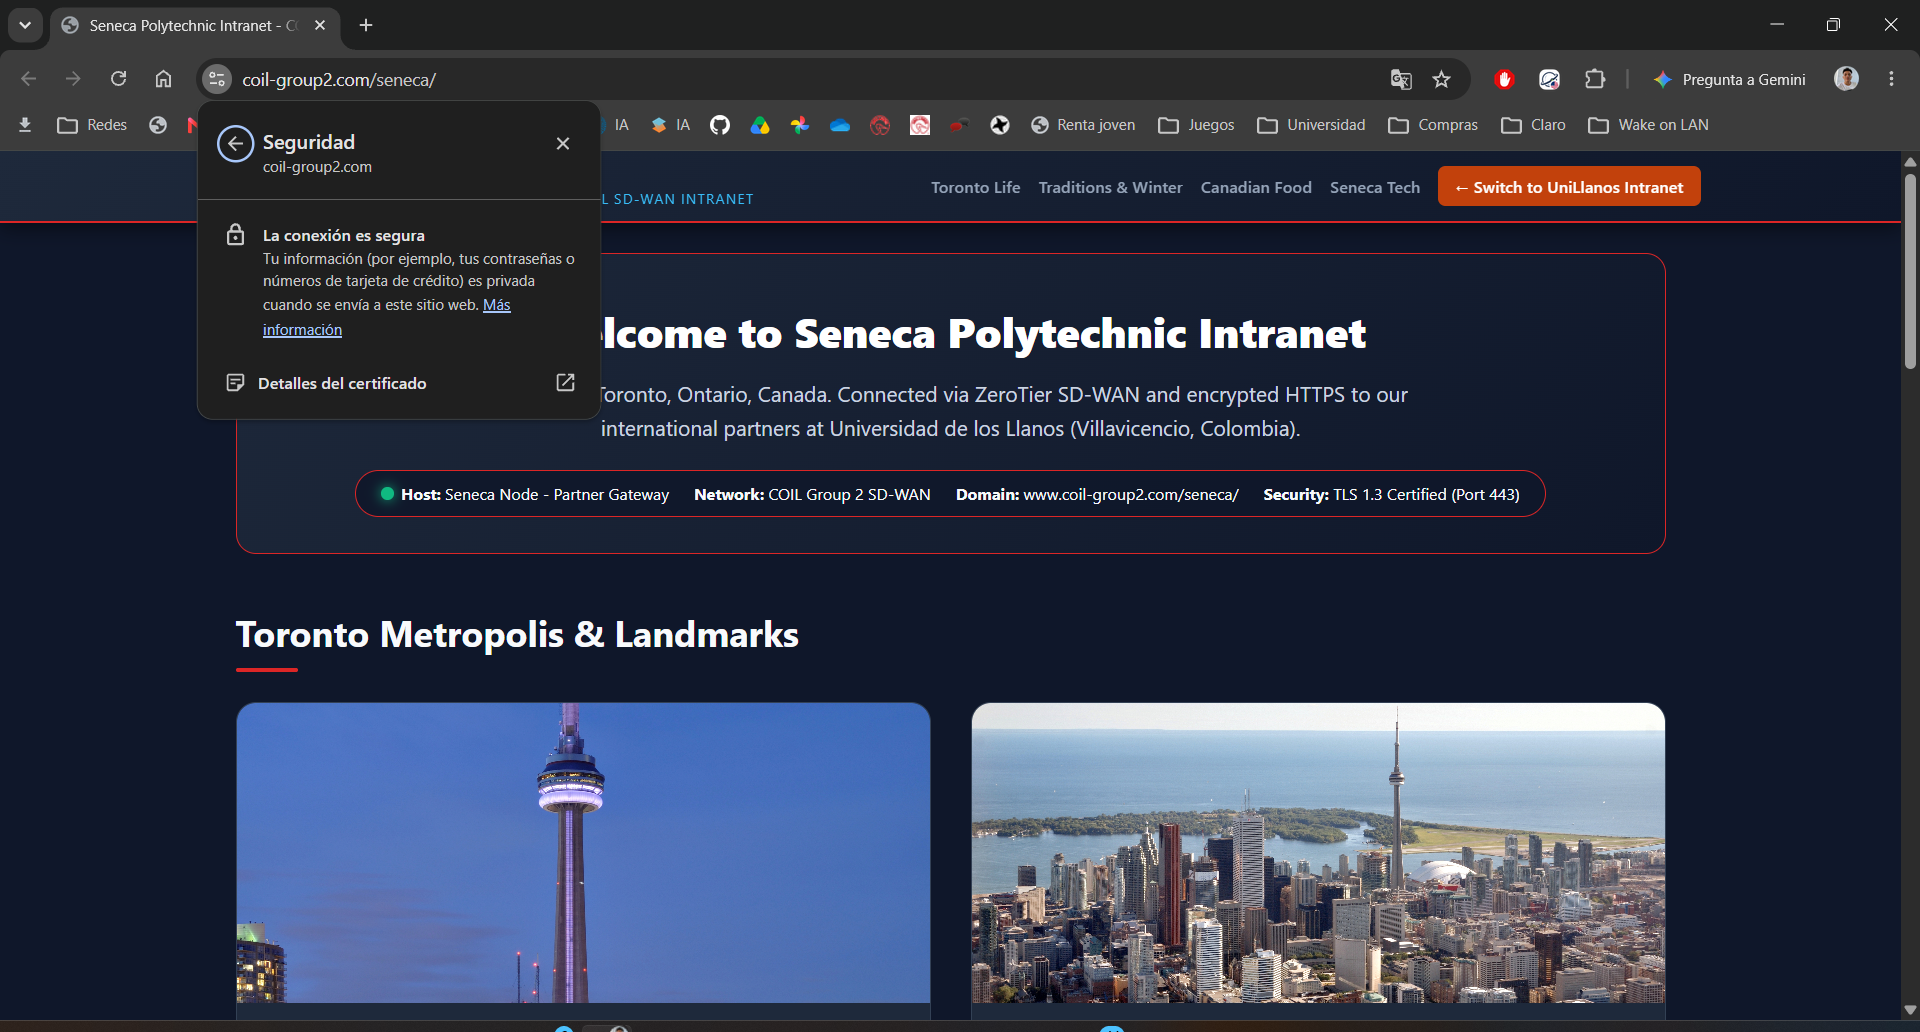
\includegraphics[width=0.90\textwidth]{figuras/cert_chrome_trusted_fresh.png}
\caption{Live Google Chrome verification on Windows navigating to \texttt{https://www.coil-group2.com/seneca/} with the site security panel open, demonstrating trusted HTTPS status and zero certificate warnings after Root CA installation (bonus objective).}
\label{fig:cert_chrome_trusted}
\end{figure*}

\begin{figure*}[htbp]
\centering
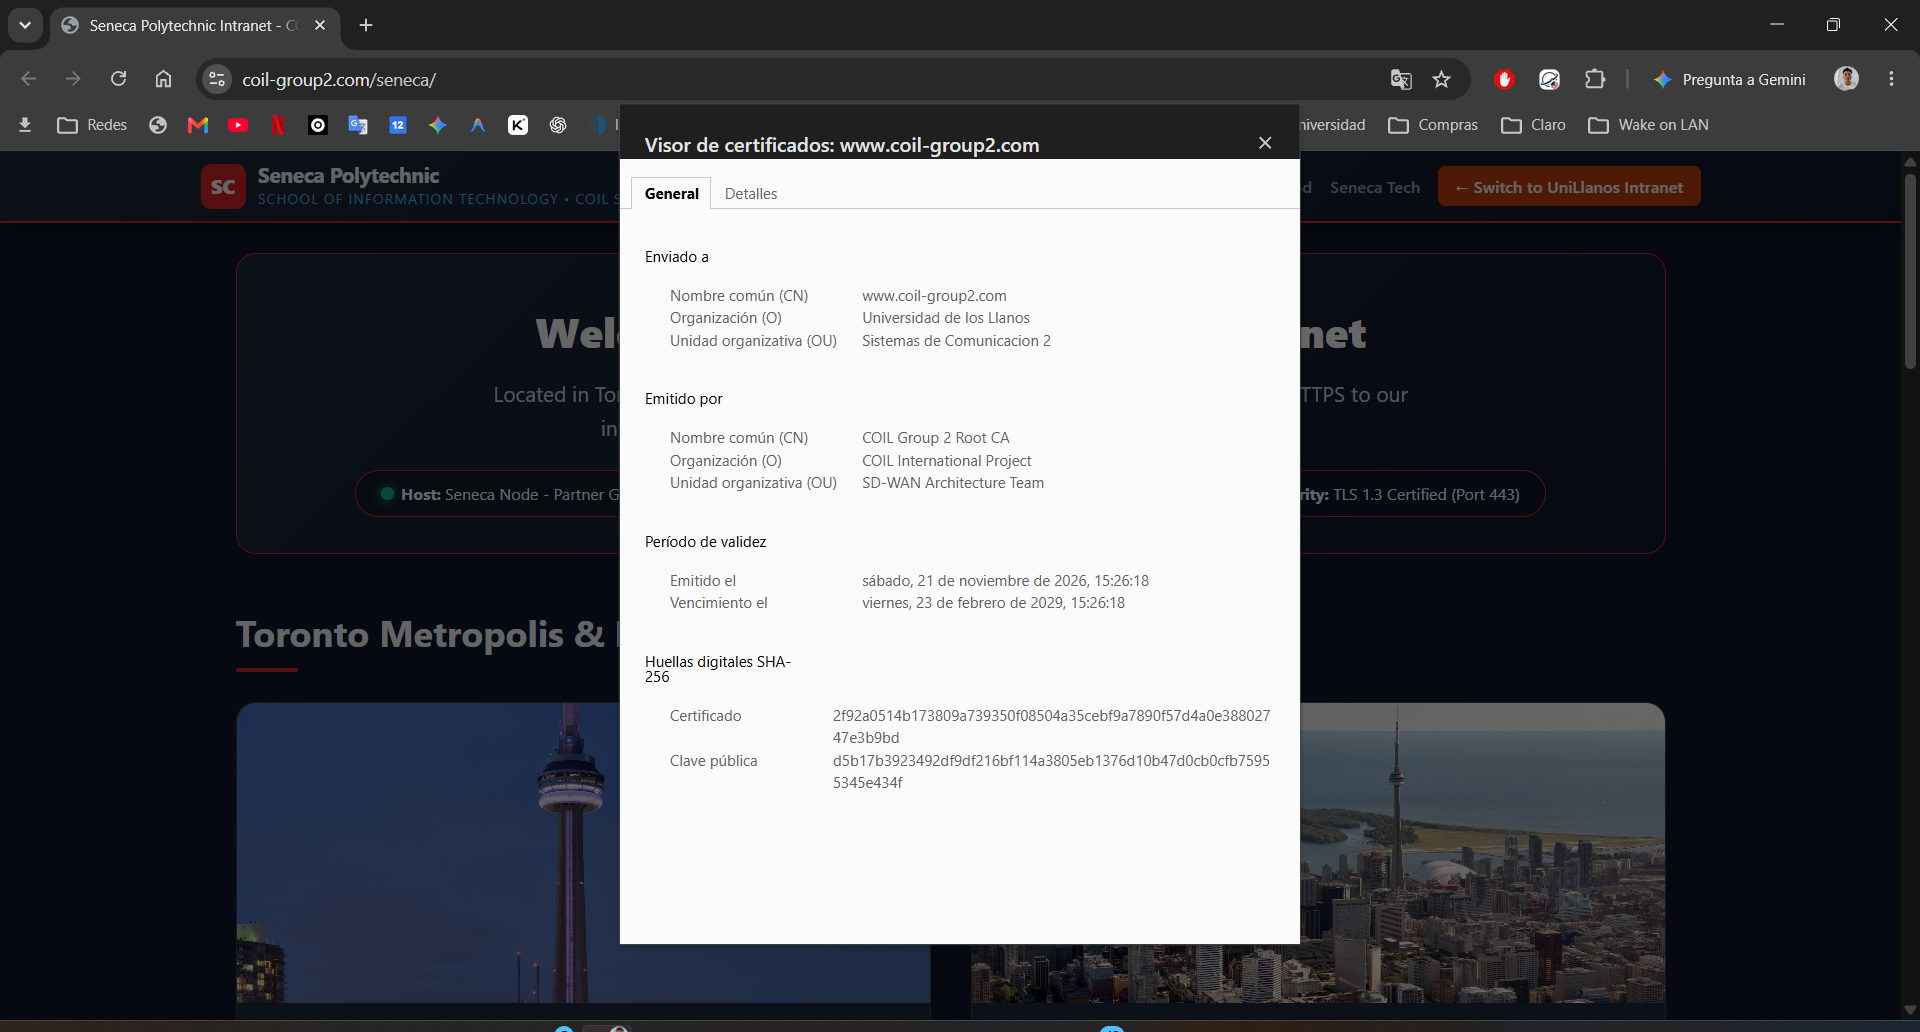
\includegraphics[width=0.90\textwidth]{figuras/cert_viewer_details_fresh.png}
\caption{Native X.509 Certificate Viewer inspection confirming the validated trust chain from \texttt{COIL Group 2 Root CA} to leaf certificate \texttt{www.coil-group2.com} with SHA-256 RSA-2048 signatures and SAN extensions.}
\label{fig:cert_viewer}
\end{figure*}

\begin{figure}[htbp]
\centering
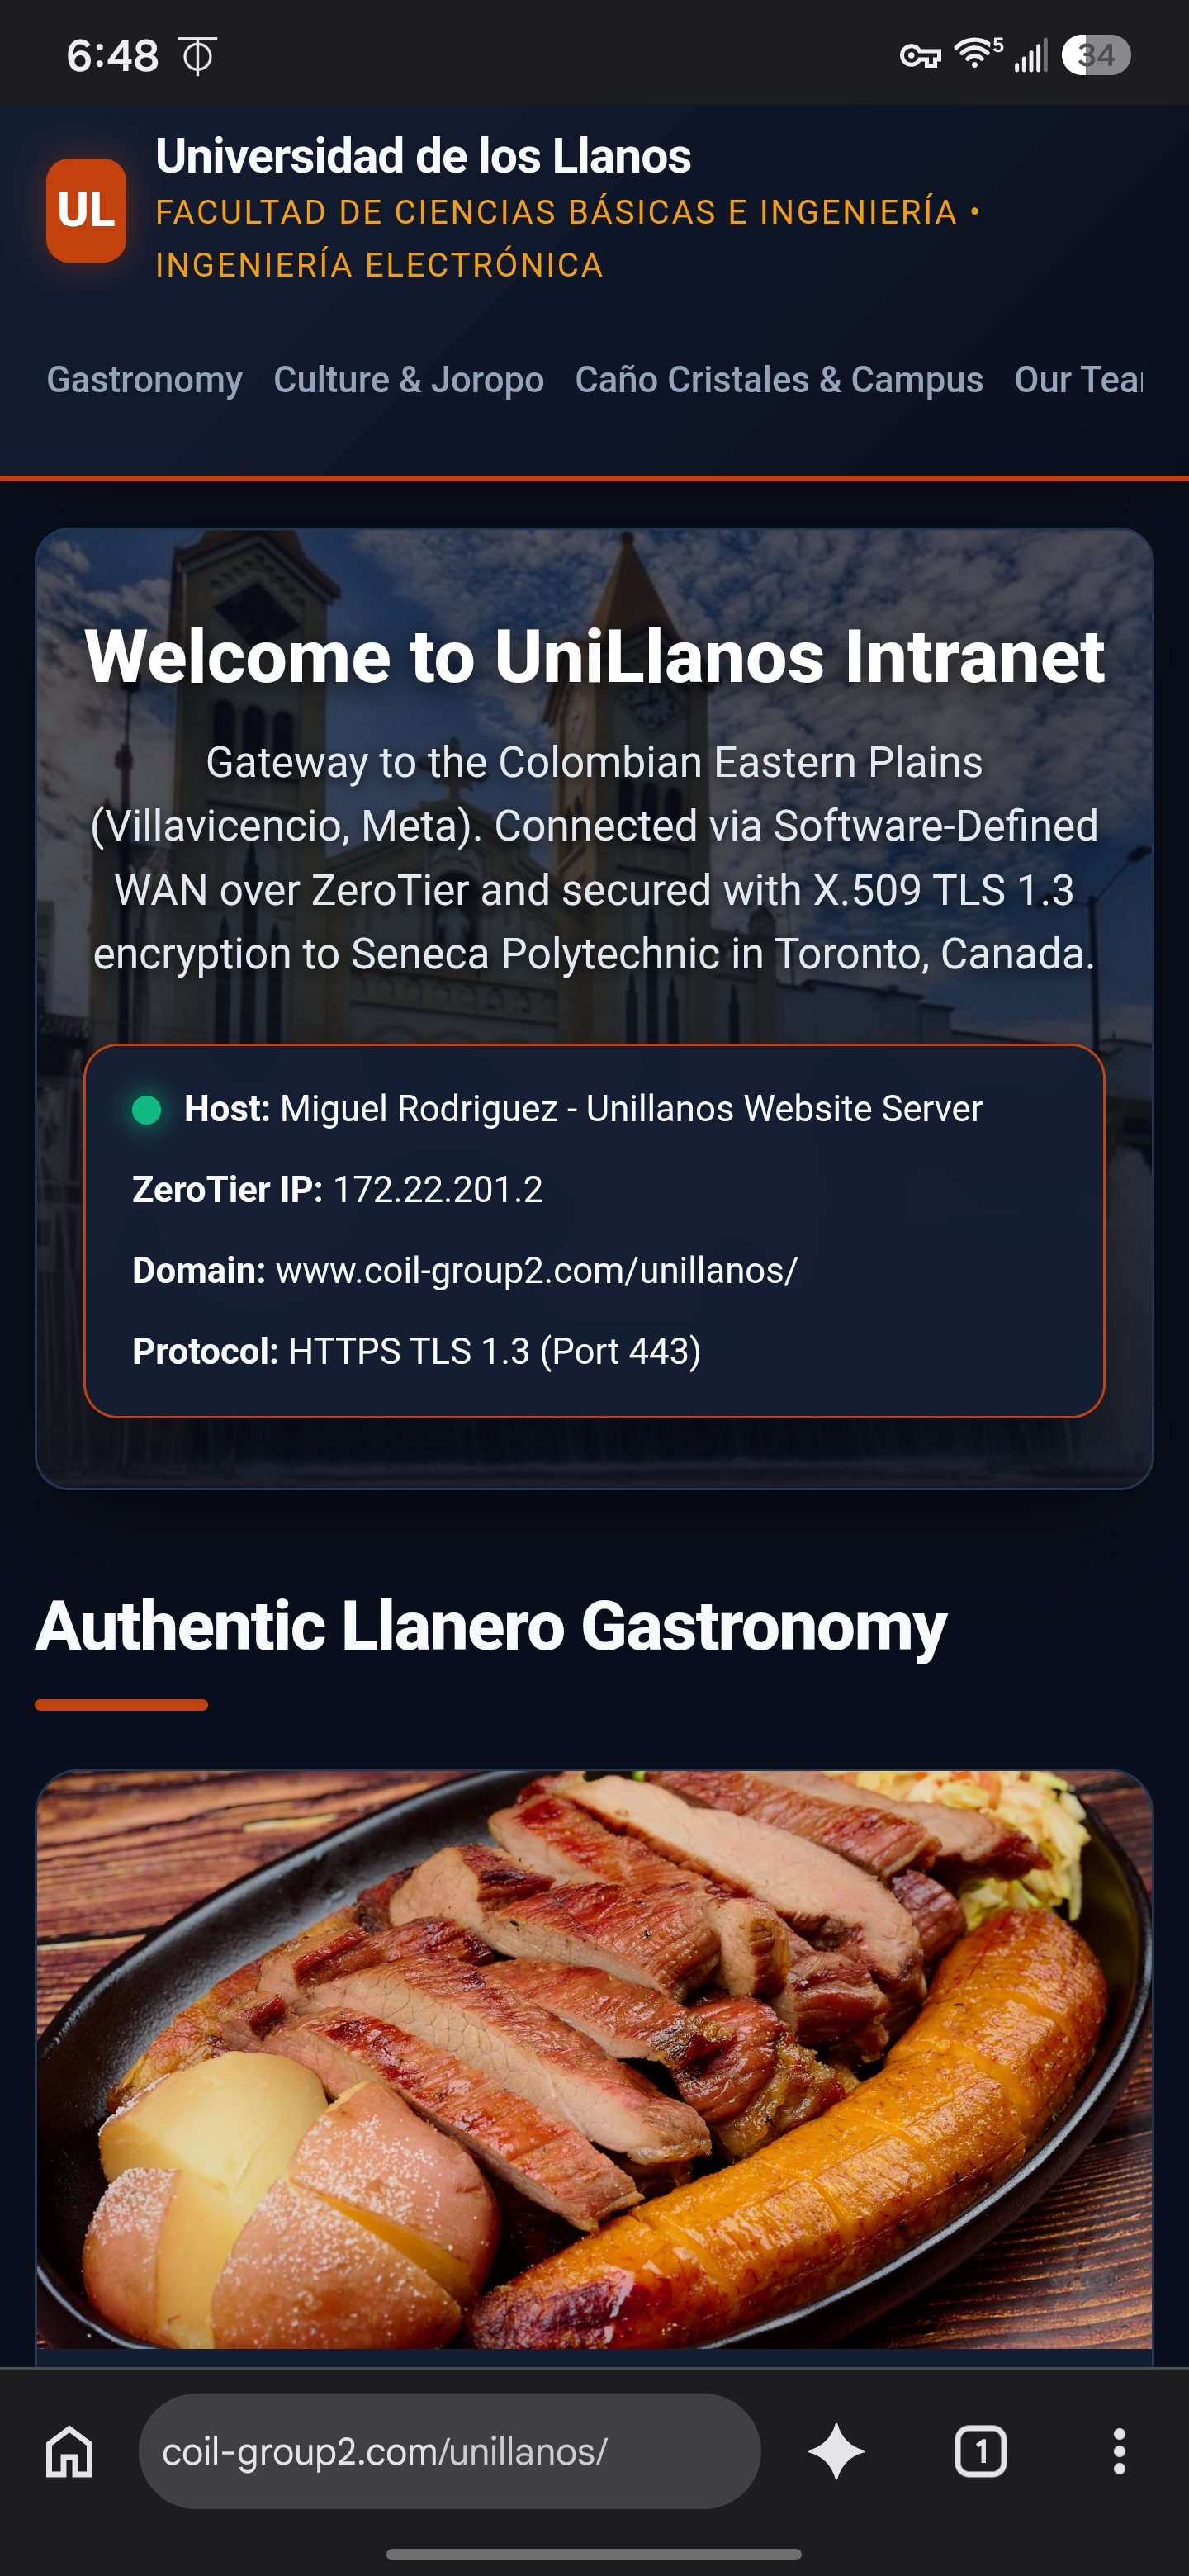
\includegraphics[width=0.58\columnwidth]{figuras/cert_mobile_android.jpg}
\caption{Cross-platform mobile verification on Android (Samsung Galaxy S24+, ZeroTier VPN active in status bar) accessing \texttt{www.coil-group2.com/unillanos/} over TLS~1.3 with the Root CA installed.}
\label{fig:cert_mobile}
\end{figure}

\subsection{Manual 4 (15\%): Authoritative and Forwarding DNS Server Configuration}
\label{subsec:manual4_dns}

To enable seamless domain-based navigation (\texttt{www.coil-group2.com/unillanos/} and \texttt{www.coil-group2.com/seneca/}) across all SD-WAN nodes without relying solely on manual IP entry, a dedicated Python DNS daemon (\texttt{modulo2/dns/dns\_server.py}) was implemented using the \texttt{dnslib} packet engine in compliance with RFC~1034~\cite{rfc1034}, RFC~1035~\cite{rfc1035}, and RFC~2308~\cite{rfc2308}. Figure~\ref{fig:dns_flowchart} illustrates the server's four-way packet-processing pipeline and host integration parameters.

\begin{figure*}[htbp]
\centering
% Local semantic palette (self-contained for drop-in inclusion in any preamble)
\definecolor{dnsNavy}{HTML}{1B365D}
\definecolor{dnsNavyBg}{HTML}{EEF4FB}
\definecolor{dnsBlue}{HTML}{1D4ED8}
\definecolor{dnsBlueBg}{HTML}{EFF6FF}
\definecolor{dnsTeal}{HTML}{0F766E}
\definecolor{dnsTealBg}{HTML}{F0FDFA}
\definecolor{dnsAmber}{HTML}{B45309}
\definecolor{dnsAmberBg}{HTML}{FFFBEB}
\definecolor{dnsRed}{HTML}{B91C1C}
\definecolor{dnsRedBg}{HTML}{FEF2F2}
\definecolor{dnsSlate}{HTML}{334155}
\definecolor{dnsMuted}{HTML}{64748B}
\definecolor{dnsPanelBg}{HTML}{F8FAFC}
\definecolor{dnsBorder}{HTML}{CBD5E1}

\resizebox{0.96\textwidth}{!}{%
\begin{tikzpicture}[
    >=Stealth,
    font=\scriptsize,
    node distance=0.55cm and 0.72cm,
    % Base box styles
    procbox/.style={
        rectangle,
        rounded corners=4pt,
        draw=dnsNavy,
        fill=dnsNavyBg,
        line width=0.85pt,
        text width=3.48cm,
        align=center,
        inner xsep=5pt,
        inner ysep=5pt,
        text=dnsSlate
    },
    parsebox/.style={
        procbox,
        draw=dnsSlate,
        fill=dnsPanelBg
    },
    decision/.style={
        diamond,
        aspect=2.2,
        draw=dnsBlue,
        fill=dnsBlueBg,
        line width=0.9pt,
        text width=2.45cm,
        align=center,
        inner xsep=3pt,
        inner ysep=3pt,
        text=dnsNavy
    },
    outcard/.style={
        rectangle,
        rounded corners=4pt,
        line width=0.9pt,
        text width=5.15cm,
        align=left,
        inner xsep=6pt,
        inner ysep=5pt,
        text=dnsSlate
    },
    outteal/.style={outcard, draw=dnsTeal, fill=dnsTealBg},
    outamber/.style={outcard, draw=dnsAmber, fill=dnsAmberBg},
    outred/.style={outcard, draw=dnsRed, fill=dnsRedBg},
    fwdbox/.style={
        rectangle,
        rounded corners=4pt,
        draw=dnsBlue,
        fill=dnsBlueBg,
        line width=0.9pt,
        text width=2.85cm,
        align=left,
        inner xsep=6pt,
        inner ysep=5pt,
        text=dnsSlate
    },
    relaybox/.style={
        rectangle,
        rounded corners=4pt,
        draw=dnsBlue,
        fill=dnsPanelBg,
        line width=0.9pt,
        text width=1.65cm,
        align=center,
        inner xsep=5pt,
        inner ysep=5pt,
        text=dnsSlate
    },
    dropbox/.style={
        rectangle,
        rounded corners=3pt,
        draw=dnsRed,
        dashed,
        fill=dnsRedBg,
        line width=0.75pt,
        text width=2.95cm,
        align=center,
        inner xsep=4pt,
        inner ysep=4pt,
        text=dnsRed
    },
    egressbox/.style={
        rectangle,
        rounded corners=4pt,
        draw=dnsNavy,
        fill=dnsNavyBg,
        line width=0.95pt,
        text width=2.15cm,
        align=center,
        inner xsep=5pt,
        inner ysep=6pt,
        text=dnsNavy
    },
    % Connectors & badges
    flow/.style={->, >=Stealth, line width=0.85pt, color=dnsNavy},
    flowteal/.style={->, >=Stealth, line width=0.95pt, color=dnsTeal},
    flowamber/.style={->, >=Stealth, line width=0.9pt, color=dnsAmber},
    flowred/.style={->, >=Stealth, line width=0.9pt, color=dnsRed},
    flowblue/.style={->, >=Stealth, line width=0.9pt, color=dnsBlue},
    dropflow/.style={->, >=Stealth, dashed, line width=0.75pt, color=dnsRed},
    yesbadge/.style={
        rectangle,
        rounded corners=2pt,
        fill=white,
        draw=dnsTeal,
        line width=0.55pt,
        inner xsep=3pt,
        inner ysep=1.5pt,
        font=\tiny\bfseries,
        text=dnsTeal
    },
    nobadge/.style={
        rectangle,
        rounded corners=2pt,
        fill=white,
        draw=dnsSlate,
        line width=0.55pt,
        inner xsep=3pt,
        inner ysep=1.5pt,
        font=\tiny\bfseries,
        text=dnsSlate
    },
    yesredbadge/.style={
        yesbadge,
        draw=dnsRed,
        text=dnsRed
    },
    yesamberbadge/.style={
        nobadge,
        draw=dnsAmber,
        text=dnsAmber
    },
    nobluebadge/.style={
        nobadge,
        draw=dnsBlue,
        text=dnsBlue
    },
    zonebox/.style={
        rectangle,
        rounded corners=6pt,
        draw=dnsBorder,
        fill=white,
        line width=0.85pt
    },
    zonehdr/.style={
        font=\footnotesize\bfseries,
        text=dnsNavy,
        inner sep=1pt
    },
    paramcard/.style={
        rectangle,
        rounded corners=4pt,
        draw=dnsBorder,
        fill=dnsPanelBg,
        line width=0.8pt,
        align=left,
        inner xsep=6pt,
        inner ysep=5pt,
        text=dnsSlate
    }
]

% ==============================================================================
% 1. TOP ZONE: PACKET-HANDLING DECISION PIPELINE (Right-to-Left by Construction)
% ==============================================================================

% Column 4: Four Resolution Lanes
\node[outteal] (out_a) at (0,0) {
    {\color{dnsTeal}\textbf{Authoritative \texttt{A} Record}} \hfill {\tiny\texttt{AA=1, NOERROR}}\\[2pt]
    Answer: \texttt{172.22.201.2} $\cdot$ TTL = \qty{300}{\second}\\
    Measured SD-WAN RTT: \textbf{\qty{0.53}{\milli\second}}
};

\node[outamber, below=0.38cm of out_a] (out_nodata) {
    {\color{dnsAmber}\textbf{RFC 2308 \texttt{NODATA + SOA}}} \hfill {\tiny\texttt{NOERROR, 0 Ans}}\\[2pt]
    Non-\texttt{A}/\texttt{ANY} (\texttt{AAAA} [28], \texttt{HTTPS} [65])\\
    Prevents Android \texttt{netd} \texttt{FORMERR} via \texttt{SOA} (\qty{300}{\second})
};

\node[outred, below=0.52cm of out_nodata] (out_nx) {
    {\color{dnsRed}\textbf{Authoritative \texttt{NXDOMAIN + SOA}}} \hfill {\tiny\texttt{RCODE=3}}\\[2pt]
    Unknown \texttt{*.coil-group2.com} subdomain\\
    Auth \texttt{SOA} negative cache (\texttt{TTL = \qty{300}{\second}})
};

\node[fwdbox, below=0.38cm of out_nx.south west, anchor=north west] (fwd_udp) {
    {\color{dnsBlue}\textbf{Upstream Forwarder}}\\[2pt]
    Raw UDP $\rightarrow$ \texttt{8.8.8.8:53}\\
    Socket timeout: \qty{2.0}{\second}
};

\node[relaybox, anchor=east] (out_relay) at (out_a.east |- fwd_udp.east) {
    {\color{dnsBlue}\textbf{Relay Reply}}\\[2pt]
    Pass upstream\\response
};

\node[dropbox, below=0.38cm of fwd_udp, text width=2.85cm] (drop_timeout) {
    Timeout / Error: Silent Drop
};

% Column 3: Secondary Decisions (Centered on Lane Pairs)
\coordinate (mid_dec1a) at ($(out_a.west)!0.5!(out_nodata.west)$);
\node[decision, anchor=east] (dec1a) at ($(mid_dec1a)+(-1.00cm,0)$) {
    \texttt{qtype in}\\[1pt]\texttt{(A, ANY)}?
};

\coordinate (mid_dec2) at ($(out_nx.west)!0.5!(fwd_udp.west)$);
\node[decision, anchor=east] (dec2) at ($(mid_dec2)+(-1.00cm,0)$) {
    Subdomain of\\[1pt]\texttt{coil-group2.com}?
};

% Column 2: Primary Decision (Centered between Dec 1a and Dec 2)
\coordinate (mid_dec1) at ($(dec1a.west)!0.5!(dec2.west)$);
\node[decision, anchor=east] (dec1) at ($(mid_dec1)+(-1.00cm,0)$) {
    \texttt{qname in}\\[1pt]\texttt{DOMAINS}?
};

% Column 1: Ingress, Parsing & Error Drop
\node[parsebox, left=0.72cm of dec1.west] (parser) {
    {\color{dnsNavy}\textbf{Parse \& Normalize}}\\[2pt]
    \texttt{DNSRecord.parse(data)}\\
    Lowercase \texttt{qname} (strip `\texttt{.}'), \texttt{qtype}
};

\node[procbox, above=0.55cm of parser] (ingress) {
    {\color{dnsNavy}\textbf{UDP Ingress Socket}}\\[2pt]
    Bind \texttt{0.0.0.0:53} (\texttt{recvfrom(4096)})\\
    \texttt{SIO\_UDP\_CONNRESET=False}
};

\node[dropbox, below=0.55cm of parser] (drop_invalid) {
    Invalid Packet: Silent Drop
};

% Column 5: Unified Client Egress Collector
\coordinate (egress_rail_x) at ($(out_a.east)+(0.48cm,0)$);
\coordinate (egress_top) at (egress_rail_x |- out_a.east);
\coordinate (egress_mid) at ($(out_a.east)!0.5!(out_relay.east)$);
\coordinate (egress_bot) at (egress_rail_x |- out_relay.east);
\coordinate (egress_hub) at (egress_rail_x |- egress_mid);

\node[egressbox, right=0.42cm of egress_hub] (egress) {
    \textbf{Client Reply}\\[2pt]
    \texttt{sendto(pkt, addr)}\\
    SD-WAN Peer
};

% ==============================================================================
% 2. ORTHOGONAL CONNECTORS & EDGE BADGES (Zero Absolute Coords, Zero Piercing)
% ==============================================================================

% Ingress -> Parser -> Dec1
\draw[flow] (ingress.south) -- (parser.north);
\draw[flow] (parser.east) -- (dec1.west);
\draw[dropflow] (parser.south) -- node[right, font=\tiny, text=dnsRed, xshift=2pt] {Parse Error} (drop_invalid.north);

% Dec1 -> Dec1a / Dec2
\draw[flowteal] (dec1.north) |- (dec1a.west);
\coordinate (b_dec1_yes) at ($(dec1.east |- dec1a.west)!0.5!(dec1a.west)$);
\node[yesbadge] at (b_dec1_yes) {YES};

\draw[flowblue] (dec1.south) |- (dec2.west);
\coordinate (b_dec1_no) at ($(dec1.east |- dec2.west)!0.5!(dec2.west)$);
\node[nobadge] at (b_dec1_no) {NO};

% Dec1a -> Out A / Out NODATA
\draw[flowteal] (dec1a.north) |- (out_a.west);
\coordinate (b_dec1a_yes) at ($(dec1a.east |- out_a.west)!0.5!(out_a.west)$);
\node[yesbadge] at (b_dec1a_yes) {YES};

\draw[flowamber] (dec1a.south) |- (out_nodata.west);
\coordinate (b_dec1a_no) at ($(dec1a.east |- out_nodata.west)!0.5!(out_nodata.west)$);
\node[yesamberbadge] at (b_dec1a_no) {NO};

% Dec2 -> Out NXDOMAIN / Forwarder
\draw[flowred] (dec2.north) |- (out_nx.west);
\coordinate (b_dec2_yes) at ($(dec2.east |- out_nx.west)!0.5!(out_nx.west)$);
\node[yesredbadge] at (b_dec2_yes) {YES};

\draw[flowblue] (dec2.south) |- (fwd_udp.west);
\coordinate (b_dec2_no) at ($(dec2.east |- fwd_udp.west)!0.5!(fwd_udp.west)$);
\node[nobluebadge] at (b_dec2_no) {NO};

% Forwarder -> Relay & Timeout Drop
\draw[flowblue] (fwd_udp.east) -- (out_relay.west);
\draw[dropflow] (fwd_udp.south) -- node[right, font=\tiny, text=dnsRed, xshift=2pt] {\texttt{resp=None}} (drop_timeout.north);

% Egress Collector Rail -> Client Reply
\draw[line width=0.85pt, color=dnsNavy] (egress_top) -- (egress_bot);
\draw[line width=0.85pt, color=dnsTeal] (out_a.east) -- (egress_rail_x |- out_a.east);
\draw[line width=0.85pt, color=dnsAmber] (out_nodata.east) -- (egress_rail_x |- out_nodata.east);
\draw[line width=0.85pt, color=dnsRed] (out_nx.east) -- (egress_rail_x |- out_nx.east);
\draw[line width=0.85pt, color=dnsBlue] (out_relay.east) -- (egress_rail_x |- out_relay.east);
\foreach \pt in {egress_top, egress_bot, egress_hub} {
    \fill[dnsNavy] (\pt) circle (1.4pt);
}
\fill[dnsAmber] (egress_rail_x |- out_nodata.east) circle (1.4pt);
\fill[dnsRed] (egress_rail_x |- out_nx.east) circle (1.4pt);
\draw[flow] (egress_hub) -- (egress.west);

% Pipeline Bounding Box & Section A Header
\node[fit=(ingress)(parser)(drop_invalid)(dec1)(dec1a)(dec2)(out_a)(out_nodata)(out_nx)(fwd_udp)(drop_timeout)(out_relay)(egress), inner sep=0pt] (pipe_bbox) {};
\node[zonehdr, anchor=south west] (hdr_a) at ($(pipe_bbox.north west)+(0,0.22cm)$) {
    A. Authoritative \& Forwarding Packet-Handling Pipeline (\texttt{modulo2/dns/dns\_server.py} $\cdot$ \texttt{dnslib} Engine)
};

\begin{pgfonlayer}{bg}
\node[zonebox, fit=(pipe_bbox)(hdr_a), inner sep=8pt] (zone_a) {};
\end{pgfonlayer}

% ==============================================================================
% 3. BOTTOM ZONE: 3-COLUMN SYSTEM PARAMETERS & WINDOWS/ZEROTIER INTEGRATION
% ==============================================================================

\node[zonehdr, anchor=north west] (hdr_b) at ($(zone_a.south west)+(8pt,-0.40cm)$) {
    B. Zone Table, RFC 2308 SOA Authority Parameters \& Windows / ZeroTier Host Integration
};

% Compute equal widths for 3 flush parameter cards spanning zone_a width (minus inner padding)
\path let \p1 = (zone_a.west), \p2 = (zone_a.east),
          \n1 = {(\x2 - \x1 - 16pt - 0.70cm)/3 - 12pt} in
    node[paramcard, anchor=north west, text width=\n1, minimum height=2.35cm] (card_domains) at ($(hdr_b.south west)+(0,-0.16cm)$) {
        {\color{dnsTeal}\textbf{1. Authoritative \texttt{DOMAINS} Map}}\\[2pt]
        {\color{dnsBorder}\rule{\linewidth}{0.5pt}}\\[3pt]
        \begin{tabular*}{\linewidth}{@{}l@{\extracolsep{\fill}}r@{}}
        \texttt{www.coil-group2.com} & \texttt{172.22.201.2} \\
        \texttt{coil-group2.com} & \texttt{172.22.201.2} \\
        \texttt{unillanos.coil-group2.com} & \texttt{172.22.201.2} \\
        \texttt{seneca.coil-group2.com} & \texttt{172.22.201.2} \\
        \end{tabular*}\\[4pt]
        {\tiny\color{dnsMuted} Records: \texttt{QTYPE.A / ANY} $\cdot$ TTL: \qty{300}{\second} $\cdot$ \texttt{NOERROR}}
    }
    node[paramcard, anchor=north west, text width=\n1, minimum height=2.35cm] (card_soa) at ($(card_domains.north east)+(0.35cm,0)$) {
        {\color{dnsAmber}\textbf{2. \texttt{SOA} Authority (\texttt{coil-group2.com})}}\\[2pt]
        {\color{dnsBorder}\rule{\linewidth}{0.5pt}}\\[3pt]
        \begin{tabular*}{\linewidth}{@{}l@{\extracolsep{\fill}}r@{}}
        Primary NS (\texttt{MNAME}): & \texttt{ns.coil-group2.com} \\
        Admin (\texttt{RNAME}): & \texttt{admin.coil-group2.com} \\
        Serial / Min TTL: & \texttt{2026112101} / \qty{300}{\second} \\
        Ref / Ret / Exp: & \qty{3600}{\second} / \qty{600}{\second} / \qty{86400}{\second} \\
        \end{tabular*}\\[4pt]
        {\tiny\color{dnsMuted} Returned in \texttt{auth} section (\qty{300}{\second}) for \texttt{NODATA}/\texttt{NXDOMAIN}}
    }
    node[paramcard, anchor=north west, text width=\n1, minimum height=2.35cm] (card_host) at ($(card_soa.north east)+(0.35cm,0)$) {
        {\color{dnsNavy}\textbf{3. Windows \& ZeroTier SD-WAN Integration}}\\[2pt]
        {\color{dnsBorder}\rule{\linewidth}{0.5pt}}\\[3pt]
        \textbf{ICS Port Release:} Stop \texttt{SharedAccess} (frees UDP/53).\\[1.5pt]
        \textbf{Firewall Rule:} Allow inbound \texttt{COIL\_DNS\_53} (UDP/53).\\[1.5pt]
        \textbf{ZeroTier Push:} Net \texttt{abfd31bd47affa39} pushes domain \texttt{coil-group2.com} \& NS \texttt{172.22.201.2} (\texttt{hosts} fallback).
    };

\begin{pgfonlayer}{bg}
\node[zonebox, fit=(hdr_b)(card_domains)(card_soa)(card_host), inner sep=8pt] (zone_b) {};
\end{pgfonlayer}

\end{tikzpicture}%
}
\caption{Packet-handling decision pipeline and authoritative zone configuration of the \texttt{dnslib}-based DNS daemon (\texttt{modulo2/dns/}\allowbreak\texttt{dns\_server.py}). Incoming UDP/53 datagrams are parsed, normalized, and routed across four deterministic branches: authoritative \texttt{A} resolution (\texttt{172.22.201.2}, TTL~=~\qty{300}{\second}, measured SD-WAN RTT~=~\qty{0.53}{\milli\second}), RFC~2308 \texttt{NODATA+SOA} responses preventing Android \texttt{netd} \texttt{FORMERR} faults on \texttt{AAAA}/\texttt{HTTPS} queries, \texttt{NXDOMAIN+SOA} negative caching for unregistered subdomains, and raw UDP forwarding to \texttt{8.8.8.8:53} (\qty{2.0}{\second} timeout) for external domains.}
\label{fig:dns_flowchart}
\end{figure*}


\subsubsection{Step 1: Authoritative Zone and RFC 2308 Negative Caching Engine}
The DNS daemon binds \texttt{UDP 0.0.0.0:53} (disabling Windows UDP connection-reset exceptions via \texttt{SIO\_UDP\_CONNRESET = False}) and maintains an authoritative dictionary mapping all four project hostnames (\texttt{www.coil-group2.com}, \texttt{coil-group2.com}, \texttt{unillanos.coil-group2.com}, and \texttt{seneca.coil-group2.com}) to \texttt{172.22.201.2} with a \qty{300}{\second} TTL:
\begin{itemize}
    \item \textbf{Type \texttt{A} (1) and \texttt{ANY} (255) Queries:} Returns an authoritative \texttt{NOERROR} answer with \texttt{AA=1} and \texttt{rdata=A("172.22.201.2")}.
    \item \textbf{Type \texttt{AAAA} (28) and \texttt{HTTPS} (65) Queries (\texttt{NODATA+SOA}):} Modern Chromium and Android (\texttt{netd}) resolvers issue parallel \texttt{AAAA} and \texttt{HTTPS} queries alongside \texttt{A} lookups. Under RFC~2308~\cite{rfc2308}, returning an empty answer section without an Authority \texttt{SOA} record causes Android \texttt{netd} to abort with \texttt{FORMERR}. The server therefore appends \texttt{SOA("ns.coil-group2.com", "admin.coil-group2.com", (2026112101, 3600, 600, 86400, 300))} in the authority section.
    \item \textbf{Unregistered Subdomains (\texttt{NXDOMAIN+SOA}):} Queries matching \texttt{*.coil-group2.com} outside the authoritative dictionary receive \texttt{RCODE.NXDOMAIN} with the authoritative \texttt{SOA} record.
    \item \textbf{External Internet Queries:} Non-COIL domains are forwarded over UDP to Google Public DNS (\texttt{8.8.8.8:53}, \qty{2.0}{\second} timeout) and relayed transparently back to the client.
\end{itemize}

\subsubsection{Step 2: Windows Port 53 Binding, Firewall Rules, and Headless Persistence}
On Windows 11, the Internet Connection Sharing service (\texttt{SharedAccess}) can reserve UDP port 53. Free port 53, open inbound firewall rules (\texttt{COIL\_DNS\_53}), and register the headless Scheduled Task (\texttt{COIL\_DNS\_Daemon} under \texttt{S4U} logon):

\begin{lstlisting}[caption={Provisioning UDP port 53, firewall rules, and persistent S4U DNS daemon.},label={lst:manual4_service}]
Stop-Service SharedAccess -Force -ErrorAction SilentlyContinue
New-NetFirewallRule -DisplayName "COIL_DNS_53" -Direction Inbound `
  -Protocol UDP -LocalPort 53 -Action Allow
$action = New-ScheduledTaskAction -Execute "python.exe" `
  -Argument '-u "modulo2\dns\dns_server.py"'
$principal = New-ScheduledTaskPrincipal -UserId (whoami) `
  -LogonType S4U -RunLevel Highest
Register-ScheduledTask -TaskName "COIL_DNS_Daemon" -Action $action `
  -Principal $principal -Force
Start-ScheduledTask -TaskName "COIL_DNS_Daemon"
\end{lstlisting}

\subsubsection{Step 3: ZeroTier DNS Push and Client Verification}
In ZeroTier Central (Figure~\ref{fig:zerotier_settings}), configure \texttt{SERVERS: 172.22.201.2} under the DNS panel. On Android clients, enable \textit{Use Network DNS} inside the ZeroTier One app and set Android \textit{Private DNS} to \textit{Off} so DNS-over-TLS does not bypass the SD-WAN resolver; on Windows clients without ZeroTier DNS push enabled, execute \texttt{modulo2/dns/setup\_hosts.ps1} as a deterministic local fallback. Live verification from both \texttt{172.22.201.2} and remote gateway \texttt{172.22.31.69} confirmed authoritative \texttt{A} and \texttt{SOA} resolution:

\begin{lstlisting}[caption={Live authoritative DNS verification for Type A and Type AAAA queries.},label={lst:manual4_verify}]
PS C:\> Resolve-DnsName www.coil-group2.com -Server 172.22.201.2 -Type A
Name                 Type   TTL   Section    IPAddress
----                 ----   ---   -------    ---------
www.coil-group2.com  A      300   Answer     172.22.201.2

PS C:\> Resolve-DnsName www.coil-group2.com -Server 172.22.201.2 -Type AAAA
Name             Type  TTL  Section    PrimaryServer       NameAdministrator     SerialNumber
----             ----  ---  -------    -------------       -----------------     ------------
coil-group2.com  SOA   300  Authority  ns.coil-group2.com  admin.coil-group2.com 2026112101
\end{lstlisting}

Figure~\ref{fig:ws_dns} presents the live Wireshark dissection of Frames~1 and~2 captured on the ZeroTier virtual adapter (\texttt{dns} display filter), confirming transaction ID \texttt{0x9121}, authoritative flag \texttt{AA=1}, resolved address \texttt{172.22.201.2} (\texttt{TTL = 300 s}), and a round-trip resolution latency of \qty{0.5346}{\milli\second}.

\begin{figure*}[htbp]
\centering
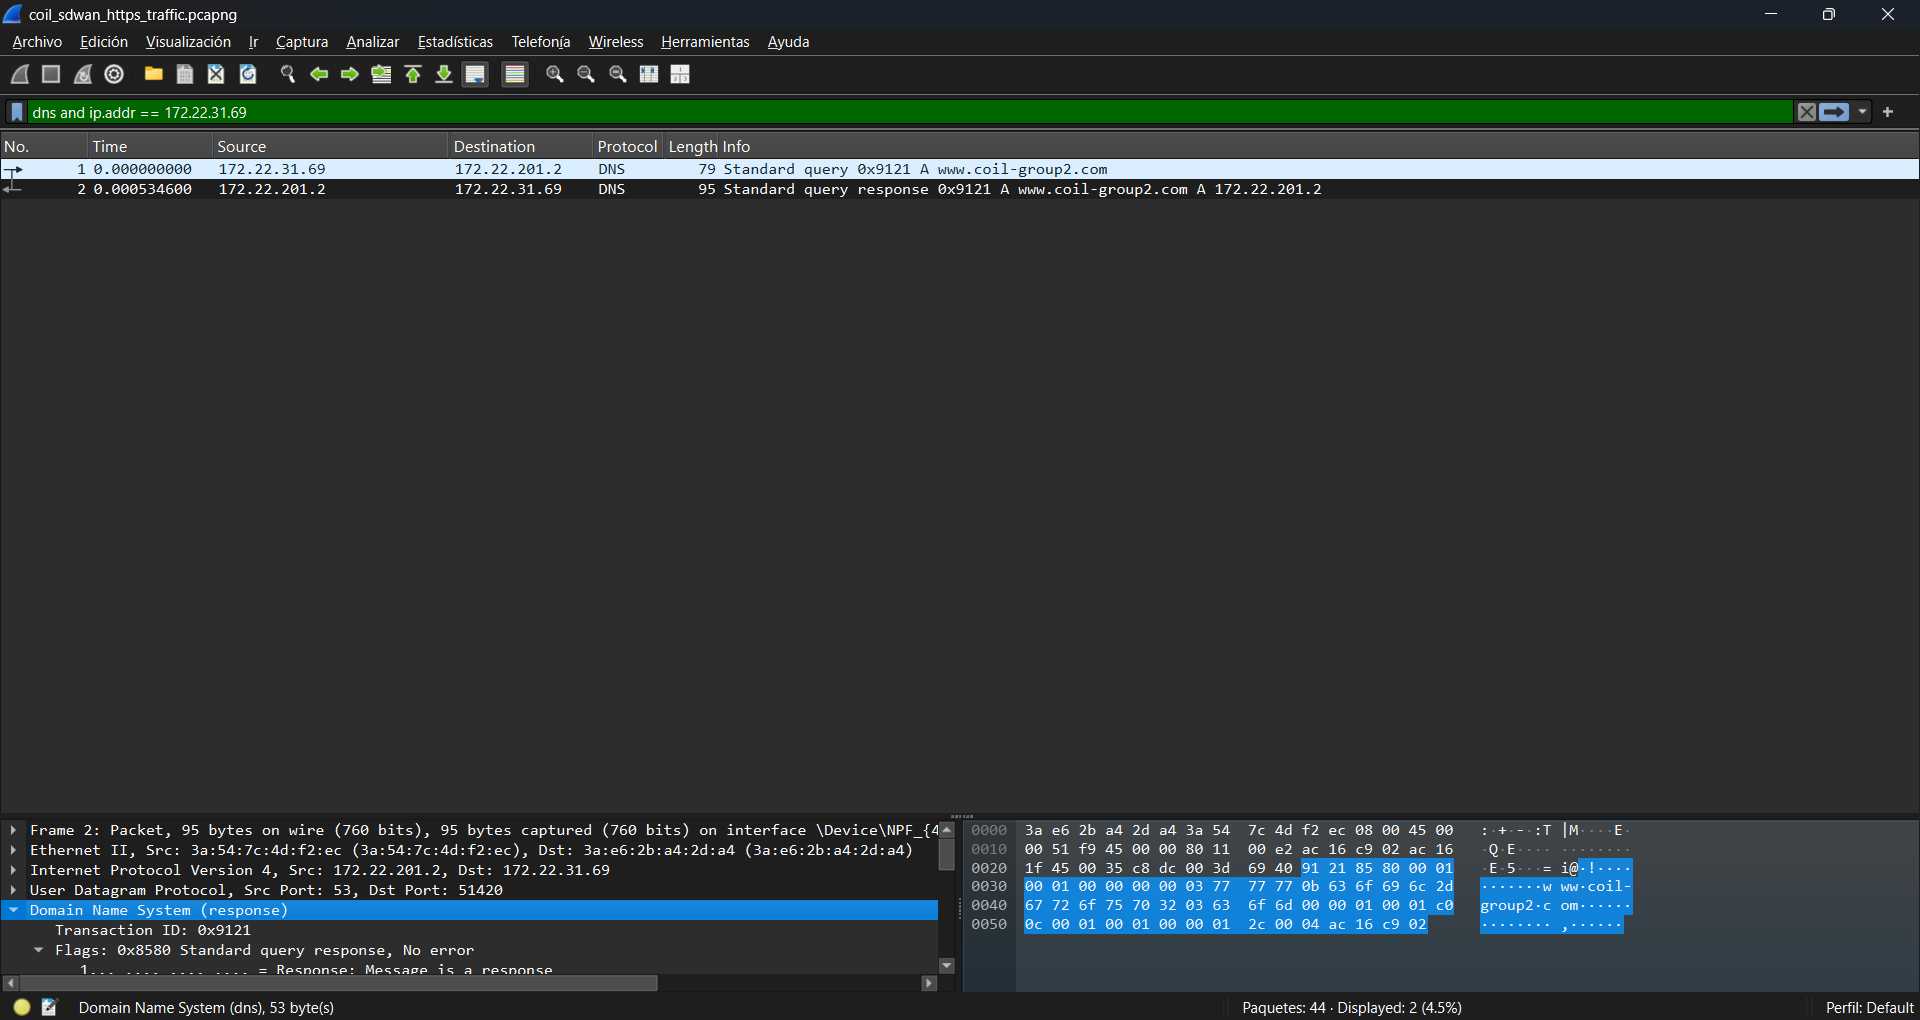
\includegraphics[width=0.92\textwidth]{figuras/wireshark_5_dns_resolution.png}
\caption{Wireshark protocol dissection of the live SD-WAN DNS query and authoritative response (Frames~1--2, Transaction ID \texttt{0x9121}, \qty{0.5346}{\milli\second} RTT) resolving \texttt{www.coil-group2.com} to \texttt{172.22.201.2} over UDP port 53.}
\label{fig:ws_dns}
\end{figure*}

\section{Quantitative Engineering Analysis and Discussion}
\label{sec:discussion}

Rather than reiterating the provisioning procedures or raw telemetry tables documented in the preceding sections, this section evaluates cross-layer performance deviations against theoretical protocol baselines and diagnoses the physical and operating-system failure modes encountered during live SD-WAN deployment. Table~\ref{tab:quantitative_comparison} synthesizes the six governing engineering metrics measured across the ZeroTier overlay, authoritative DNS daemon, TLS~1.3 transport stack, and Wireshark forensic capture.

\begin{table*}[t]
\centering
\caption{Cross-Layer Quantitative Comparison: Theoretical Baselines vs.\ Live Measured SD-WAN Telemetry and Relative Deviation}
\label{tab:quantitative_comparison}
\footnotesize
\setlength{\tabcolsep}{4.5pt}
\renewcommand{\arraystretch}{1.24}
\begin{tabularx}{\textwidth}{@{}
  >{\hsize=0.72\hsize\raggedright\arraybackslash}X
  >{\hsize=0.96\hsize\raggedright\arraybackslash}X
  >{\hsize=1.18\hsize\raggedright\arraybackslash}X
  >{\hsize=1.14\hsize\raggedright\arraybackslash}X
  @{}}
\toprule
\textbf{Metric / Subsystem} & \textbf{Theoretical / Spec.\ Baseline} & \textbf{Live Measured SD-WAN Value} & \textbf{Relative Deviation / Overhead} \\
\midrule
\textbf{Maximum Segment Size (MSS)} &
Standard Ethernet (\qty{1500}{\byte} MTU $\rightarrow$ \qty{1460}{\byte} MSS)~\cite{rfc9293,tanenbaum2021} &
Tuned ZeroTier overlay (\qty{1300}{\byte} MTU $\rightarrow$ \qty{1260}{\byte} MSS in Frames~3--4) &
$-\qty{13.70}{\percent}$ intentional reduction (\qty{200}{\byte} encapsulation headroom preventing cellular/PPPoE fragmentation) \\
\addlinespace[4pt]
\textbf{LAN P2P Overlay Latency} &
Direct Gigabit Ethernet ($\approx \qty{0.50}{\milli\second}$ RTT) &
ZeroTier UDP-9993 P2P tunnel (\qty{6.0}{\milli\second}--\qty{10.0}{\milli\second} avg.\ ICMP RTT; \qty{14.21}{\milli\second} TCP \texttt{SYN}/\texttt{SYN-ACK}) &
$+\qty{5.5}{\milli\second}$ to $+\qty{9.5}{\milli\second}$ over bare LAN due to overlay encryption and user-space TUN/TAP processing~\cite{zerotier2024} \\
\addlinespace[4pt]
\textbf{WAN P2P Overlay Latency} &
ZeroTier LAN overlay baseline (\qty{10.0}{\milli\second} avg.\ RTT) &
Partner ISP WAN leaf (\nolinkurl{172.22.100.11} / \nolinkurl{172.22.164.74}: \qty{23.0}{\milli\second}--\qty{31.0}{\milli\second} avg.\ ICMP RTT, \qty{0}{\percent} loss) &
$+\qty{13.0}{\milli\second}$ to $+\qty{21.0}{\milli\second}$ Internet routing propagation delta across cross-ISP underlay hops \\
\addlinespace[4pt]
\textbf{Authoritative DNS Lookup} &
Local OS cache / \texttt{hosts} lookup ($< \qty{0.10}{\milli\second}$) &
Live remote \texttt{dnslib} UDP-53 query (\qty{0.5346}{\milli\second} in Frame~2) &
Sub-millisecond SD-WAN name resolution (\qty{0.27}{\percent} of \qty{200}{\milli\second} interactive budget)~\cite{rfc1035,kurose2017} \\
\addlinespace[4pt]
\textbf{TLS~1.3 + TCP Wire Overhead} &
Plaintext HTTP payload (\qty{15470}{\byte} Seneca HTML; \qty{15734}{\byte} with HTTP headers) &
\qty{22785}{\byte} bidirectional wire bytes across 36 TCP/TLS frames (\num{19135} server seq.\ bytes; \qty{19134}{\byte} TCP payload) &
\qty{47.29}{\percent} total framing + TLS~1.3 1-RTT handshake/AEAD record overhead (\qty{7315}{\byte} delta over HTML payload)~\cite{rfc8446} \\
\addlinespace[4pt]
\textbf{PCAP Deliverable vs.\ Limit} &
Rubric upper cap (\qty{10.0}{\mega\byte} = \qty{10240}{\kilo\byte}) &
Captured \nolinkurl{coil_sdwan_https_traffic.pcapng} (\qty{24.81}{\kilo\byte} = \qty{25408}{\byte}) &
\qty{99.76}{\percent} safety margin below cap (\qty{0.24}{\percent} budget utilization)~\cite{wireshark2023} \\
\bottomrule
\end{tabularx}
\end{table*}

\subsection{Cross-Layer Framing, Latency Cascade, and Wire-Byte Accounting}
\label{subsec:cross_layer_analysis}

Tuning the ZeroTier virtual interface MTU from the Ethernet standard of \qty{1500}{\byte} down to \qty{1300}{\byte} lowers the negotiated TCP Maximum Segment Size (MSS) observed in Frames~3--4 of \nolinkurl{coil_sdwan_https_traffic.pcapng} according to
\begin{equation}
\Delta_{\text{MSS}} = \frac{1260 - 1460}{1460} \times \qty{100}{\percent} = -\qty{13.70}{\percent},
\label{eq:mss_delta}
\end{equation}
subtracting \qty{40}{\byte} of combined IPv4 (\qty{20}{\byte}) and TCP (\qty{20}{\byte}) header overhead from each bound~\cite{rfc9293}. This deliberate \qty{200}{\byte} encapsulation margin prevents Path MTU Discovery (PMTUD) blackholing and outer IP fragmentation when ZeroTier Virtual Layer~1 (VL1) wraps each virtual frame inside outer IPv4/UDP-9993 headers and cryptographic framing over residential PPPoE DSL links (\qty{1492}{\byte} MTU) or cellular carrier tunnels~\cite{kozierok2005,zerotier2024}. On the virtual wire itself, per-segment L2--L4 payload efficiency shifts only slightly from $1460/1514 = \qty{96.43}{\percent}$ on bare Ethernet to $1260/1314 = \qty{95.89}{\percent}$ on the overlay (a \qty{0.54}{\percent} per-frame efficiency trade-off), representing an advantageous compromise for heterogeneous WAN traversal.

Across the time domain, comparing Table~\ref{tab:icmp_rtt} with the live packet capture isolates each layer's latency contribution. While direct Gigabit Ethernet achieves $\approx \qty{0.50}{\milli\second}$ round-trip times, local ZeroTier P2P forwarding (\texttt{172.22.201.2} $\leftrightarrow$ \texttt{172.22.31.69}) adds $+\qty{5.5}{\milli\second}$ to $+\qty{9.5}{\milli\second}$ (\qty{6.0}{\milli\second}--\qty{10.0}{\milli\second} average ICMP RTT), reflecting user-space TUN/TAP context switches and per-packet tunnel encryption~\cite{zerotier2024}. The TCP \texttt{SYN} to \texttt{SYN-ACK} handshake in Frames~3--4 measures \qty{14.21}{\milli\second}, incorporating socket-buffer allocation alongside the overlay RTT. Extending across public residential ISPs (\texttt{181.51.34.123} to \texttt{181.51.34.104} toward \nolinkurl{172.22.100.11} and \nolinkurl{172.22.164.74}) contributes an additional $+\qty{13.0}{\milli\second}$ to $+\qty{21.0}{\milli\second}$ propagation and queueing delta (\qty{23.0}{\milli\second}--\qty{31.0}{\milli\second} average ICMP RTT) with \qty{0}{\percent} packet loss. Meanwhile, remote UDP-53 resolution of \nolinkurl{www.coil-group2.com} via \texttt{dns\_server.py} (Frames~1--2) completes in \qty{0.5346}{\milli\second}---consuming just \qty{0.27}{\percent} of a \qty{200}{\milli\second} interactive latency budget and avoiding multi-hop recursive root lookups~\cite{forouzan2013,kurose2017}.

At the cryptographic and transport layers, dissecting the 36 TCP/TLS frames (Frames~3--38, \texttt{tcp.stream == 0}) accounts exactly for every wire byte. Delivering the \qty{15470}{\byte} Seneca HTML document (\nolinkurl{modulo2/sitio_web/seneca/index.html}) with HTTP/1.1 headers from \texttt{COIL-DualIntranet/2.0} produces \qty{15734}{\byte} of plaintext application data (\qty{264}{\byte} HTTP metadata)~\cite{rfc9110}. Over the encrypted TCP stream, the server transmits \qty{19134}{\byte} of TCP payload (advancing relative sequence numbers to \num{19135} prior to \texttt{FIN}, verified by \texttt{Ack=19136} in Frame~36) and the client sends \qty{1683}{\byte} (TLS~1.3 \texttt{ClientHello} with SNI, \texttt{Finished}, and the encrypted \texttt{GET} request), totaling \qty{20817}{\byte} of bidirectional TCP payload. Adding Ethernet/IPv4/TCP headers across the 36 frames ($34 \times \qty{54}{\byte} + 2 \times \qty{66}{\byte} = \qty{1968}{\byte}$, including \qty{12}{\byte} of TCP options in Frames~3--4) yields \qty{22785}{\byte} on the wire. Relative to the raw HTML resource, the single-session protocol and 1-RTT TLS~1.3 handshake/AEAD record overhead is
\begin{equation}
\delta_{\text{wire}} = \frac{22785 - 15470}{15470} \times \qty{100}{\percent} = \qty{47.29}{\percent},
\label{eq:wire_overhead}
\end{equation}
corresponding to a \qty{7315}{\byte} total protocol delta (\qty{264}{\byte} HTTP headers, \qty{5083}{\byte} TLS~1.3 handshake/certificate/AEAD framing and client request, and \qty{1968}{\byte} L2--L4 headers). Because the 1-RTT TLS~1.3 handshake and X.509 chain transmission represent a fixed per-connection cost~\cite{rfc8446,rfc5280}, session resumption or larger multimedia transfers rapidly amortize this overhead toward the baseline AEAD and L2--L4 framing floor. Finally, the \qty{24.81}{\kilo\byte} (\qty{25408}{\byte}) trace file occupies only
\begin{equation}
U_{\text{pcap}} = \frac{\qty{24.8125}{\kilo\byte}}{\qty{10240}{\kilo\byte}} \times \qty{100}{\percent} = \qty{0.24}{\percent}
\label{eq:pcap_util}
\end{equation}
of the \qty{10.0}{\mega\byte} rubric limit, preserving a \qty{99.76}{\percent} size margin.

\subsection{Root-Cause Troubleshooting and Deployment Failure Modes}
\label{subsec:troubleshooting}

Transitioning the SD-WAN from local desktop prototypes to multi-device Windows and Android operation uncovered five subtle cross-layer failure modes. Each discrepancy required protocol-level or operating-system root-cause isolation rather than superficial configuration retries:

\begin{enumerate}
    \item \textbf{Search Domain Suffix Loop and Android Private DNS Bypass:} Initially populating ZeroTier Central's \textit{Search Domain} field with \texttt{coil-group2.com} caused Android \texttt{netd} and Chromium stub resolvers to append the search suffix onto already-qualified queries, synthesizing malformed FQDNs (\nolinkurl{www.coil-group2.com.coil-group2.com}) and triggering \texttt{DNS\_PROBE\_STARTED} failures~\cite{rfc1034,rfc1035}. Simultaneously, Android Private DNS (DNS-over-TLS on TCP port~853) bypassed ZeroTier's pushed UDP-53 server (\texttt{172.22.201.2}) by sending queries directly to public DoT resolvers. Clearing the Search Domain field in ZeroTier Central while retaining \texttt{172.22.201.2} as the managed DNS server, alongside temporarily disabling Android Private DNS on mobile test clients, restored deterministic SD-WAN resolution.

    \item \textbf{Missing RFC~2308 Authority SOA on Authoritative \texttt{NODATA} Replies:} Even after valid \texttt{A} answers were served, Android \texttt{netd} rejected queries for \nolinkurl{www.coil-group2.com} with internal \texttt{FORMERR} errors. Dual-stack mobile resolvers emit concurrent \texttt{Type~1 (A)}, \texttt{Type~28 (AAAA)}, and \texttt{Type~65 (HTTPS)} service-binding queries~\cite{rfc1035}. When early DNS logic returned empty packets (zero Answer and zero Authority sections) for unsupported \texttt{AAAA} and \texttt{HTTPS} queries, strict stub validators classified the empty replies as malformed rather than valid negative answers. Injecting an explicit authoritative \texttt{SOA\_RECORD} (\texttt{ns.coil-group2.com}, \texttt{admin.coil-group2.com}) via \texttt{reply.add\_auth()} in \nolinkurl{modulo2/dns/dns_server.py} for both \texttt{NODATA} and \texttt{NXDOMAIN} paths achieved strict RFC~2308 compliance~\cite{rfc2308}.

    \item \textbf{Windows Winsock \texttt{TCP RST} on \texttt{shutdown(SHUT\_WR)} and Unread Buffers:} Early HTTPS tests intermittently aborted with \texttt{ERR\_CONNECTION\_CLOSED} due to server-emitted \texttt{TCP RST} segments. Python's standard \texttt{socketserver.TCPServer} calls \texttt{socket.shutdown(socket.SHUT\_WR)} inside \texttt{shutdown\_request()} prior to closing; on Windows Winsock2, issuing \texttt{SHUT\_WR} or closing an underlying socket while unread TLS \texttt{close\_notify} alert bytes remain in the kernel receive buffer triggers an immediate \texttt{TCP RST} instead of a graceful four-way teardown~\cite{rfc9293,rfc8446}. In \nolinkurl{modulo2/servidor/server_https.py}, \texttt{DualIntranetHandler} enforces \texttt{Connection: close} (\texttt{self.close\_connection = True}), while \texttt{NonBlockingSSLThreadingServer} overrides \texttt{process\_request\_thread} to perform TLS wrapping inside worker threads and terminate directly via \texttt{close\_request()} without premature \texttt{SHUT\_WR}. Frames~35--38 of the final capture confirm a clean \texttt{FIN,ACK}/\texttt{ACK}/\texttt{FIN,ACK}/\texttt{ACK} closure with zero \texttt{RST} frames.

    \item \textbf{Headless \texttt{pythonw.exe} Null \texttt{sys.stderr} and SSH Job-Object Termination:} Attempting background execution with \texttt{pythonw.exe} crashed \texttt{server\_https.py} upon the first client request because detached GUI-subsystem processes set \texttt{sys.stderr} to \texttt{None}, causing \texttt{DualIntranetHandler.log\_message()} to raise an \texttt{AttributeError} on \texttt{sys.stderr.write()}. Conversely, launching standard \texttt{python.exe} over remote OpenSSH sessions bound the daemon to an interactive Windows Job Object flagged with \nolinkurl{JOB_OBJECT_LIMIT_KILL_ON_JOB_CLOSE}, terminating both web and DNS services immediately upon SSH exit. Hosting both daemons under Windows Task Scheduler with \texttt{S4U} non-interactive logon running \texttt{python.exe} headlessly eliminated Job-Object teardown while preserving valid I/O streams.

    \item \textbf{Windows Schannel Revocation Check Failures (\texttt{CRYPT\_E\_NO\_\allowbreak REVOCATION\_CHECK}):} Following installation of \nolinkurl{COIL_Group2_Root_CA.crt}, desktop Chromium and Android browsers validated the leaf SAN chain immediately without warnings. However, native Windows WinHTTP/Schannel CLI probes (e.g., \texttt{curl.exe}) failed because the offline OpenSSL policy (\nolinkurl{modulo2/certificados/openssl.cnf}) omits live CRL Distribution Points and OCSP Authority Information Access (AIA) URLs~\cite{rfc5280,openssl2024}. Passing \texttt{--ssl-no-revoke} in automated Schannel diagnostic scripts bypassed offline revocation lookups while preserving cryptographic signature and SAN verification against the trusted Root CA.
\end{enumerate}

\section{Conclusions and Future Work}
\label{sec:conclusions}

This engineering project fulfilled all four measurable objectives established in Section~\ref{sec:introduction}, validating an end-to-end encrypted international SD-WAN and dual-intranet architecture across Windows and Android endpoints:

\begin{enumerate}
    \item \textbf{Private SD-WAN Overlay Interconnection:} Five endpoints (\num{3} active Windows hosts and \num{2} Android handsets, \num{0} unauthorized devices) were interconnected over ZeroTier network \texttt{abfd31bd47affa39} (\texttt{172.22.0.0/16}) at a tuned \qty{1300}{\byte} MTU (\qty{1260}{\byte} MSS, $-\qty{13.70}{\percent}$ vs.\ Ethernet). Live telemetry achieved \qty{0}{\percent} packet loss across desktop P2P links, with \qty{6.0}{\milli\second}--\qty{10.0}{\milli\second} LAN RTT and \qty{23.0}{\milli\second}--\qty{31.0}{\milli\second} cross-ISP WAN RTT.

    \item \textbf{Dual Cultural Intranets over TLS~1.3 and Private PKI:} The threaded \texttt{COIL-DualIntranet/2.0} server delivered both the Universidad de los Llanos and Seneca Polytechnic portals (\qty{15470}{\byte} Seneca HTML payload) under TLS~1.3 (\nolinkurl{TLS_AES_256_GCM_SHA384}, 1-RTT) anchored to \texttt{COIL Group 2 Root CA}. Installing the 2048-bit Root CA eliminated all browser security warnings on Windows and Android clients, incurring a quantified \qty{47.29}{\percent} single-session wire overhead (\qty{22785}{\byte} bidirectional total vs.\ \qty{15470}{\byte} raw HTML).

    \item \textbf{Authoritative SD-WAN DNS Resolution:} The RFC~1035 and RFC~2308 compliant \texttt{dnslib} daemon (\texttt{dns\_server.py}) resolved \nolinkurl{www.coil-group2.com} and institutional subdomains over UDP port~53 with \texttt{NODATA+SOA} negative-caching compliance, achieving \qty{0.5346}{\milli\second} live SD-WAN lookup latency (\qty{0.27}{\percent} of a \qty{200}{\milli\second} interactive UX budget) and eliminating raw IP navigation.

    \item \textbf{Wireshark Packet Forensics Within Rubric Constraints:} Dissection of \nolinkurl{coil_sdwan_https_traffic.pcapng} (\qty{24.81}{\kilo\byte} = \qty{25408}{\byte}) consumed just \qty{0.24}{\percent} of the \qty{10.0}{\mega\byte} limit (\qty{99.76}{\percent} margin), empirically verifying \qty{1260}{\byte} MSS negotiation, a \qty{14.21}{\milli\second} TCP handshake, encrypted TLS~1.3 payload delivery, and a zero-\texttt{RST} four-way \texttt{FIN} teardown across Frames~35--38.
\end{enumerate}

As targeted future enhancements, three architectural upgrades would elevate the platform toward production carrier standards: (1)~hosting an internal OCSP responder or static CRL endpoint referenced in \nolinkurl{openssl.cnf} AIA extensions~\cite{rfc5280} so strict WinHTTP/Schannel clients validate certificates without \texttt{--ssl-no-revoke}; (2)~upgrading \texttt{COIL-DualIntranet/2.0} to HTTP/2 (\texttt{h2} ALPN) with TLS~1.3 PSK session resumption~\cite{rfc8446,rfc9110} to multiplex embedded cultural imagery and amortize the \qty{7315}{\byte} 1-RTT setup overhead; and (3)~enabling ZeroTier deterministic IPv6 \texttt{6PLANE} addressing alongside \texttt{AAAA} records in \texttt{dns\_server.py} to eliminate dual-stack \texttt{NODATA} queries on mobile carrier networks.


\renewcommand{\refname}{References}
\bibliographystyle{IEEEtran}
\bibliography{referencias}

\clearpage
\onecolumn
\appendices
\section{UniLlanos Cultural Intranet Source Code}
\label{app:unillanos_html}
Listing~\ref{lst:unillanos_html} reproduces the complete HTML5 and CSS3 implementation of the Universidad de los Llanos cultural intranet deployed at \texttt{https://www.coil-group2.com/unillanos/}.

\lstinputlisting[
  language=HTML,
  caption={Complete source code of \texttt{modulo2/sitio\_web/unillanos/index.html}.},
  label={lst:unillanos_html}
]{../sitio_web/unillanos/index.html}

\section{Seneca Polytechnic Intranet Source Code}
\label{app:seneca_html}
Listing~\ref{lst:seneca_html} presents the full institutional HTML5 and CSS3 source code for the Seneca Polytechnic partner intranet served at \texttt{https://www.coil-group2.com/seneca/}.

\lstinputlisting[
  language=HTML,
  caption={Complete source code of \texttt{modulo2/sitio\_web/seneca/index.html}.},
  label={lst:seneca_html}
]{../sitio_web/seneca/index.html}

\section{Dual Intranet Gateway Portal Source Code}
\label{app:portal_html}
Listing~\ref{lst:portal_html} documents the landing gateway page routing visitors to either institution from \texttt{https://www.coil-group2.com/}.

\lstinputlisting[
  language=HTML,
  caption={Complete source code of \texttt{modulo2/sitio\_web/portal/index.html}.},
  label={lst:portal_html}
]{../sitio_web/portal/index.html}

\section{Multi-Tenant HTTP/HTTPS Web Server}
\label{app:server_https}
Listing~\ref{lst:server_https} provides the production threaded dual-protocol HTTP/HTTPS server (\texttt{COIL-DualIntranet/2.0}) serving both intranets and distributing the Root CA bundle.

\lstinputlisting[
  language=Python,
  caption={Complete source code of \texttt{modulo2/servidor/server\_https.py}.},
  label={lst:server_https}
]{../servidor/server_https.py}

\section{Authoritative and Forwarding DNS Server}
\label{app:dns_server}
Listing~\ref{lst:dns_server} shows the RFC~1035 and RFC~2308 compliant \texttt{dnslib} daemon responsible for resolving COIL domains over UDP port 53 and forwarding external queries to \texttt{8.8.8.8}.

\lstinputlisting[
  language=Python,
  caption={Complete source code of \texttt{modulo2/dns/dns\_server.py}.},
  label={lst:dns_server}
]{../dns/dns_server.py}

\section{PKI and Client Deployment Automation Scripts}
\label{app:pki_scripts}
Listings~\ref{lst:openssl_cnf}, \ref{lst:install_ca_ps1}, and~\ref{lst:setup_hosts_ps1} contain the OpenSSL X.509v3 Subject Alternative Name configuration and automated PowerShell client provisioning scripts.

\begin{lstlisting}[caption={OpenSSL PKI and SAN extension policy (\texttt{modulo2/certificados/openssl.cnf}).},label={lst:openssl_cnf}]
[ req ]
default_bits        = 2048
distinguished_name  = req_distinguished_name
prompt              = no

[ req_distinguished_name ]
C   = CO
ST  = Meta
L   = Villavicencio
O   = COIL International Project
OU  = SD-WAN Architecture Team
CN  = COIL Group 2 Root CA

[ v3_ca ]
subjectKeyIdentifier   = hash
authorityKeyIdentifier = keyid:always,issuer
basicConstraints       = critical, CA:true
keyUsage               = critical, digitalSignature, cRLSign, keyCertSign

[ server_req ]
default_bits        = 2048
distinguished_name  = server_distinguished_name
prompt              = no

[ server_distinguished_name ]
C   = CO
ST  = Meta
L   = Villavicencio
O   = Universidad de los Llanos & Seneca Polytechnic
OU  = Sistemas de Comunicacion 2 - COIL
CN  = www.coil-group2.com

[ server_ext ]
subjectKeyIdentifier   = hash
authorityKeyIdentifier = keyid,issuer
basicConstraints       = CA:FALSE
keyUsage               = digitalSignature, keyEncipherment
extendedKeyUsage       = serverAuth, clientAuth
subjectAltName         = @alt_names

[ alt_names ]
DNS.1 = www.coil-group2.com
DNS.2 = coil-group2.com
DNS.3 = unillanos.coil-group2.com
DNS.4 = seneca.coil-group2.com
DNS.5 = localhost
IP.1  = 172.22.201.2
IP.2  = 172.22.31.69
IP.3  = 10.51.76.174
IP.4  = 127.0.0.1
\end{lstlisting}

\lstinputlisting[
  caption={Automated Windows Root CA trust installation script (\texttt{modulo2/certificados/install\_root\_ca.ps1}).},
  label={lst:install_ca_ps1}
]{../certificados/install_root_ca.ps1}

\lstinputlisting[
  caption={Automated Windows local hosts fallback script (\texttt{modulo2/dns/setup\_hosts.ps1}).},
  label={lst:setup_hosts_ps1}
]{../dns/setup_hosts.ps1}


\end{document}
